% Gelfand seminar notes, 1976-77: source pages P000659-P000706, P000752-P000758.
% Russian diplomatic transcription (AI-made, checked against the scans), cut page by page from the cumulative working reader A4-reader-chapters01-34-complete-first1527-separated-diplomatic-r35.
% \SourcePage{GELFAND-Pnnnnnn}{label} starts a scanned page; the second argument is the number written
% on the page, if any. Editorial notes give the page, a label and the transcriber's remark; \Unclear
% marks a doubtful reading.
\SourcePage{GELFAND-P000659}{unlabelled}
\underline{6/IX-76 г.}\quad \underline{Сем. Гельфанда.}

\underline{Что надо знать из физики?}\qquad [Справа] (\underline{По Синаю}?)
\Unclear{GELFAND-P000659}{sinai-attribution}{На правом поле «По Синаю?» с вопросительным знаком.}
\end{GelfandAdjacentEvidence}
\begin{GelfandAdjacentEvidence}{GELFAND-P000659}{2}


1. Классическая механика и гам. формализм.

\quad Арнольд (\(\leq 30\) стр.), Ландау и Лифшиц.

2. Квантовая механика и теория рассеяния.

\quad Ландау и Лифшиц, Квантовая механика (минус первые две главы).

\quad Ферми, Квантовая механика.

3. Теория поля и теория относительности.

\quad Ландау и Лифшиц, Вейнберг, Космология и теория гравитации (1–4 главы).

4. Квантовая теория поля.

[зачёркнуто]
\Incomplete{GELFAND-P000659}{cancelled-four}{Строка под пунктом 4 густо зачёркнута.}
\end{GelfandAdjacentEvidence}
\begin{GelfandAdjacentEvidence}{GELFAND-P000659}{3}


К след. разу проконсульт. с физиками и сделать на машинке.

\underline{Квантовая теория поля}

1. Вторичное квантование (Бозе и Ферми). [Вписано снизу: статистика] --- Ландау и Лифшиц.

2. Запись уравнений [вписано в выноске: поля] через континуальный интеграл,
\SourceFigure{GELFAND-P000659}{field-callout}{%
\par\smallskip
\begingroup\color{black}\GelfandFitDiagram{\begin{tikzpicture}[line width=.55pt]
\node at (0,0) {поля};
\draw (.50,.31) .. controls (.32,-.14) and (.83,.20) .. (.83,-.10)
 .. controls (.80,-.34) and (-.85,-.29) .. (-.88,-.07)
 .. controls (-.92,.09) and (-.40,.21) .. (.05,.22)
 .. controls (.25,.24) and (.41,.22) .. (.50,.31);
\end{tikzpicture}}\endgroup\par
В выноске после «уравнений» написано «поля».}
\end{GelfandAdjacentEvidence}
\begin{GelfandAdjacentEvidence}{GELFAND-P000659}{4}

ряд теории возмущений, диаграммы Фейнмана.

3. Перенормировки. --- Хепп.

4. Поля Янга--Миллса --- есть обзоры.

\underline{Гиндикин} (и Гельфанд).
\underline{Всё об \(SL(2,\mathbb R)\).}
\[
G=SL(2,\mathbb R)
\]
\[
\begin{pmatrix}\alpha&\beta\\\gamma&\delta\end{pmatrix},
\qquad \det(\,)=1
\]
(гиперболоид в \(\mathbb R^4\))
\[
\alpha\delta-\beta\gamma=1
\]
Он отвечает форме с 2-мя плюсами и 2-мя минусами:
\[
x^2+y^2-z^2-t^2=1.
\]
На гиперболоиде действует группа \(G\times G\) с пом. левых и правых сдвигов
\[
\underbrace{T_{(g_1,g_2)}g=g_1^{-1}gg_2}.
\]
\Unclear{GELFAND-P000659}{action-overwrite}{Последнее \(g_2\) густо наведено.}
\end{GelfandAdjacentEvidence}
\begin{GelfandAdjacentEvidence}{GELFAND-P000659}{5}


Любое лин. преобр., сохр. гиперб., можно записать в таком виде.

Стац. подгруппа точки \(e=\begin{pmatrix}1&0\\0&1\end{pmatrix}\)
состоит из преобр. [зачёркнуто]
\Incomplete{GELFAND-P000659}{cancelled-stabilizer}{Скобка видна, её содержимое густо перечёркнуто.}
\end{GelfandAdjacentEvidence}

вида \((g,g)\).


\Needspace{7\baselineskip}
\begin{GelfandAdjacentEvidence}{GELFAND-P000660}{1}
\SourcePage{GELFAND-P000660}{unlabelled}
[Вверху зачёркнута строка]
\Incomplete{GELFAND-P000660}{cancelled-top}{Строка густо зачёркнута. Видны отдельные штрихи букв.}
\end{GelfandAdjacentEvidence}
\begin{GelfandAdjacentEvidence}{GELFAND-P000660}{2}


\underline{Упражнение:} вычислить стац. подгр. других точек.

Рассм. ф-и на гиперболоиде.

При \(\beta\ne0\) удобны координаты [зачёркнуто: \(\alpha,\beta,\delta\)]
\(\alpha,\delta,\beta\).
\Unclear{GELFAND-P000660}{coordinates}{Первый знак зачёркнутой тройки наведён и читается предположительно.}
\end{GelfandAdjacentEvidence}
\begin{GelfandAdjacentEvidence}{GELFAND-P000660}{3}


Ф-и на гиперболоиде можно рассм. как ф-и \(\psi(\alpha,\delta,\beta)\).

Функции нужно интегрировать по инвариантной мере:
\[
dg=\frac{d\alpha\,d\beta\,d\delta}{|\beta|}
\]
(инвар. отн. движ. гиперболоида).

Будем рассматривать пр-во \(\mathcal H=L^2(G)\) относительно этой меры.
\[
\|\psi\|^2=\int|\psi(g)|^2\,dg.
\]
\underline{Задача:} разложить ф-и на [обведено и зачёркнуто: неприводимые]
подпр-ва, инвар. относительно
\Incomplete{GELFAND-P000660}{cancelled-irreducible}{Обведённая надстрочная вставка перечёркнута.}
\end{GelfandAdjacentEvidence}
\begin{GelfandAdjacentEvidence}{GELFAND-P000660}{4}

\[
T_{(g_1,g_2)}\psi(g)=\psi(g_1^{-1}gg_2).
\]
В \(\mathbb R^4\) рассматриваем гиперплоскости
\[
\xi\alpha+\eta\delta-p\beta-q\gamma=\zeta.
\]
Г. \underline{Философия:} надо разделить на \underline{серии} (алгебр. задача)

(Бернштейн, Гельфанд, Гельфанд)
\Unclear{GELFAND-P000660}{three-credits}{Фамилия «Гельфанд» записана дважды подряд.}
\end{GelfandAdjacentEvidence}
\begin{GelfandAdjacentEvidence}{GELFAND-P000660}{5}


Серии на представления --- другая (трансценд.) задача.

Этот известный пример (Bargman, Гельфанд и Граев, Молчанов, Strichartz, Виленкин
и др.) --- известно уже всё о гиперболоидах.
\Unclear{GELFAND-P000660}{example-surname}{Первая фамилия выглядит как латинское «Bargman».}
\end{GelfandAdjacentEvidence}
\begin{GelfandAdjacentEvidence}{GELFAND-P000660}{6}


На непривод. --- \underline{не надо}.

Возможны след. типы сечений.
\[
\text{I.}\quad \Delta=\begin{vmatrix}\xi&p\\q&\eta\end{vmatrix}<0
\quad\text{однополостный гиперболоид}\qquad 4\text{ параметра}
\]
\[
\text{II.}\quad \Delta=\begin{vmatrix}\xi&p\\q&\eta\end{vmatrix}>0
\]
\[
\left.
\begin{array}{rlrl}
\text{а)}&|\zeta|>2\sqrt{\Delta}&\text{однопол. гиперболоид}&4\\
\text{б)}&|\zeta|<2\sqrt{\Delta}&\text{двупол. гиперб.}&4\\
\text{в)}&|\zeta|=2\sqrt{\Delta}&\text{конус}&3
\end{array}
\right\}\ \text{параметра}
\]
\Unclear{GELFAND-P000660}{sections-count}{Числа 4, 4 и 3 написаны на правом поле и объединены скобкой.}
\end{GelfandAdjacentEvidence}
\begin{GelfandAdjacentEvidence}{GELFAND-P000660}{7}


\(\text{III.}\quad\Delta=0\) --- плоская вещь в гиперб. цилиндр\quad \(2\) параметра.
\SourceFigure{GELFAND-P000660}{degenerate-label}{%
\par\smallskip
\begingroup\color{black}\GelfandFitDiagram{\begin{tikzpicture}[line width=.55pt]
\node at (0,.19) {гиперб. параболоид};
\draw (-2.07,-.03) .. controls (-2.43,.18) and (-2.23,.48) .. (-1.96,.48)
 -- (1.96,.51) .. controls (2.20,.51) and (2.31,.03) .. (1.96,.02)
 -- (-.98,-.03) .. controls (-1.21,-.06) and (-1.38,-.13) .. (-1.48,-.32)
 .. controls (-1.46,-.12) and (-1.58,-.07) .. (-1.69,-.04) -- (-2.07,-.03);
\end{tikzpicture}}\endgroup\par
Над строкой обведено «гиперб. параболоид». Одиночный знак перед «гиперб. цилиндр» похож на «в».}
\end{GelfandAdjacentEvidence}



\Needspace{7\baselineskip}
\begin{GelfandAdjacentEvidence}{GELFAND-P000661}{1}
\SourcePage{GELFAND-P000661}{unlabelled}
\(A\) --- однопол. гиперболоид (\textit{случаи} I, IIа), 4-пар..

\(B\) --- двупол. гиперболоид (---»--- IIб), 4-пар..

[Зачёркнута отдельная буква: \(A\)?]
\Unclear{GELFAND-P000661}{cancel-letter}{Зачёркнутая буква между B и D похожа на A.}
\end{GelfandAdjacentEvidence}
\begin{GelfandAdjacentEvidence}{GELFAND-P000661}{2}


\(D\) --- конусы, 3-пар..

\(E\) --- гиперболич. параболоид (случай III), 3-пар..
\[
\psi\in\mathcal H.
\]
\[
\widehat\psi(\xi,\eta,p,q,\zeta)=
\int\psi(g)\delta(\xi\alpha+\eta\delta-p\beta-q\gamma-\zeta)\,dg.
\]
(преобр. Радона ф-и во всём пр-ве)

(Г. По технике восх. к технике раб. Г. и Наймарка 1947 г.)

\(\mathcal H_A,\mathcal H_B,\mathcal H_D,\mathcal H_E\) --- ф-и, у к-рых равны 0 интегралы
[зачёркнут знак: \(\varphi\)?] по гиперпл. данного сем-ва.
\Unclear{GELFAND-P000661}{overwritten-D}{Третий нижний индекс наведён. По контуру читается D.}
\end{GelfandAdjacentEvidence}
\begin{GelfandAdjacentEvidence}{GELFAND-P000661}{3}

\Unclear{GELFAND-P000661}{cancel-integrals}{В зачёркнутом знаке видны петля и нижний штрих, напоминающие φ.}
\end{GelfandAdjacentEvidence}
\begin{GelfandAdjacentEvidence}{GELFAND-P000661}{4}


[Зачёркнуто: Зад.?] Как описать, какие ф-и 4-х и 3-х перем. появляются?
\Unclear{GELFAND-P000661}{cancel-question}{Зачёркнутое начало вопроса предположительно читается «Зад.».}
\end{GelfandAdjacentEvidence}
\begin{GelfandAdjacentEvidence}{GELFAND-P000661}{5}


\underline{Основная теорема 1.}

[Зачёркнута формула: \(\mathcal H=\mathcal H_A\ldots\)]
\Unclear{GELFAND-P000661}{cancel-decomp}{В зачёркнутой формуле видны \(\mathcal H\), знак равенства и \(\mathcal H\) с индексом \(A\). Конечный знак не установлен.}
\end{GelfandAdjacentEvidence}
\begin{GelfandAdjacentEvidence}{GELFAND-P000661}{6}

\[
1.\quad \mathcal H=\mathcal H_A\overset{\circ}{+}\mathcal H_B.
\]
\Unclear{GELFAND-P000661}{sum-circle}{Над плюсом написан маленький кружок с наведёнными штрихами.}
\end{GelfandAdjacentEvidence}
\begin{GelfandAdjacentEvidence}{GELFAND-P000661}{7}

\Unclear{GELFAND-P000661}{sum-mark}{Слева от плюса видна также отдельная точка.}
\end{GelfandAdjacentEvidence}
\begin{GelfandAdjacentEvidence}{GELFAND-P000661}{8}

\[
2.\quad \mathcal H_A=\mathcal H_D=\mathcal H_E.
\]
Ф-я \(\widehat\psi\) удовл. ультрагиперб. ур-ю 2-го порядка, к-рое можно выписать.

Сем-ва \(A,D,E\) явл. минимальными.

Прямолин. образующие --- 3-пар. сем-во \(C\).
\Unclear{GELFAND-P000661}{ruling-adjective}{Сокращение читается «Прямолин.».}
\end{GelfandAdjacentEvidence}
\begin{GelfandAdjacentEvidence}{GELFAND-P000661}{9}

\[
\begin{pmatrix}1&z\\0&1\end{pmatrix}
\quad\text{--- пример прямой},\qquad
\begin{pmatrix}h&z\\0&h^{-1}\end{pmatrix}
\quad(h\text{ --- фиксир.})
\]
или
\[
g_1^{-1}\begin{pmatrix}1&z\\0&1\end{pmatrix}g_2
\quad\text{(общ. вид прямолин. образующей)}.
\]
\Unclear{GELFAND-P000661}{ruling-repeat}{В скобках повторено то же сокращение «прямолин.».}
\end{GelfandAdjacentEvidence}
\begin{GelfandAdjacentEvidence}{GELFAND-P000661}{10}


\(C\) --- прямолин. образующие.
\[
2'.\quad \mathcal H_A=\mathcal H_D=\mathcal H_E=\mathcal H_C.
\qquad\text{(дискретные серии)}
\]
\underline{Явное указ. проекторов и описание этих пр-в.}
\[
\alpha\delta-\beta\gamma=1.
\]
Рассм. соотв. пов. в \(\mathbb C^4\) с тем же ур-ем.
\Unclear{GELFAND-P000661}{last-referent}{Последнее сокращение перед «в» читается «пов.».}
\end{GelfandAdjacentEvidence}
\begin{GelfandAdjacentEvidence}{GELFAND-P000661}{11}


и на ней области:
\Unclear{GELFAND-P000661}{last-pronoun}{Местоимение после «на» читается «ней».}
\end{GelfandAdjacentEvidence}



\Needspace{7\baselineskip}
\begin{GelfandAdjacentEvidence}{GELFAND-P000662}{1}
\SourcePage{GELFAND-P000662}{unlabelled}
\[
\begingroup\color{black}\GelfandFitDiagram{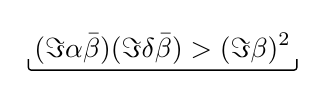
\begin{tikzpicture}[baseline=(inequality.base)]
\node[inner sep=2pt] (inequality)
  {$\displaystyle(\Im\alpha\bar\beta)(\Im\delta\bar\beta)>(\Im\beta)^2$};
\draw[line width=.5pt,rounded corners=1pt]
  ([yshift=4pt]inequality.south west) -- (inequality.south west) --
  (inequality.south east) -- ([yshift=4pt]inequality.south east);
\end{tikzpicture}}\endgroup
\qquad(1)
\]
Рассм. её в \(\mathbb C^3\).
\Unclear{GELFAND-P000662}{opening-pronoun}{Местоимение после «Рассм.» предположительно читается «её».}
\end{GelfandAdjacentEvidence}
\begin{GelfandAdjacentEvidence}{GELFAND-P000662}{2}


Она распад. на 2 обл., остовом к-рых является вещ. пр-во \(\mathbb R^3\).

Нер-во инвар. отн. дробно-лин. преобр. (одна из обл. Зигеля).

Остов \(G=SL(2,\mathbb R)\).

Области разделяются знаком скобок.

(Остов области \(D\) --- наименьшее мн-во в \(\partial D\), по ограничению на к-рое однозн. восст. ф-я, голом. в \(D\) и непр. в \(\bar D\).)

\underline{Лемма.} В \(\mathbb C^3\) с коорд. \((\alpha,\beta,\delta)\)
[зачёркнута запись] нер-во (1) выд. 2 обл. с остовами \(\mathbb R^3\) у каждой.
\Incomplete{GELFAND-P000662}{cancel-lemma}{Короткая запись после тройки координат густо зачёркнута.}
\end{GelfandAdjacentEvidence}
\begin{GelfandAdjacentEvidence}{GELFAND-P000662}{3}

\Unclear{GELFAND-P000662}{lemma-continuation}{Перед числом 2 предположительно написано «выд.» (выделяет).}
\end{GelfandAdjacentEvidence}
\begin{GelfandAdjacentEvidence}{GELFAND-P000662}{4}


\underline{Теорема.} На пов. \(\alpha\delta-\beta\gamma=1\) в
\(\mathbb C^4\) сущ. 2 инвар. отн. вещ. движ. области, имеющие остовами гиперболоид
[зачёркнут знак] \(\alpha\delta-\beta\gamma=1\) в \(\mathbb R^4\).
\Incomplete{GELFAND-P000662}{cancel-theorem}{Начальный знак слева от уравнения гиперболоида перечёркнут.}
\end{GelfandAdjacentEvidence}
\begin{GelfandAdjacentEvidence}{GELFAND-P000662}{5}

Обозначим эти области \(D_+\) и \(D_-\).

\underline{Основная теор. 2.}
\[
\psi\in\mathcal H_A\ \Longleftrightarrow\ \psi=\psi_++\psi_-,\quad\text{где}
\]
\(\psi_+\) аналит. прод. в \(D_+\), \(\psi_-\) аналит. прод. в \(D_-\).

[Над строкой: Обозн. [зачёркнут знак] подпр-ва через
\(\mathcal H_{A,+}\) и \(\mathcal H_{A,-}\).]
\Incomplete{GELFAND-P000662}{subspace-insertion}{Между «Обозн.» и «подпр-ва» зачёркнут знак с расходящимися штрихами.}
\end{GelfandAdjacentEvidence}
\begin{GelfandAdjacentEvidence}{GELFAND-P000662}{6}

\Unclear{GELFAND-P000662}{subspace-signs}{Во втором индексе длинную черту пересекает тонкий вертикальный штрих. Чтение минуса предположительное.}
\end{GelfandAdjacentEvidence}
\begin{GelfandAdjacentEvidence}{GELFAND-P000662}{7}


Проектор на \(\mathcal H_{A,+}\) задаётся ф-ией
\[
\int_G K(g_1,g_2)\psi(g_2)\,dg_2,
\]
где
\[
K(g_1,g_2)=c\,\frac{1}{[-\alpha_1\delta_2-\delta_1\alpha_2+\gamma_1\beta_2+\beta_1\gamma_2+2]^{3/2}}.
\]
\[
g_1=\begin{pmatrix}\alpha_1&\beta_1\\\gamma_1&\delta_1\end{pmatrix},
\qquad g_1\in D_+.
\]
Аналогично 2-й проектор.
\[
\mathcal H_{A,+}\cap\mathcal H_{A,-}=\{0\},
\]
т. к. [зачёркнута запись] всё в \(L^2\).
\Incomplete{GELFAND-P000662}{cancel-intersection}{Слово после «т. к.» густо зачёркнуто.}
\end{GelfandAdjacentEvidence}
\begin{GelfandAdjacentEvidence}{GELFAND-P000662}{8}


\underline{\underline{Подводная часть:}} техника интеграла Фурье.

\(K(g_1,g_2)\) --- аналог ядра Коши.

\underline{Гипотеза Арнольда.} \(D_+\) --- те, к-рые круг перев. в себя,

\(D_-\) --- те, к-рые внешн. круга [зачёркнута запись] перев. в себя,
\Incomplete{GELFAND-P000662}{cancel-circle}{Короткая запись после «круга» густо зачёркнута.}
\end{GelfandAdjacentEvidence}


\(SL(2,\mathbb R)\) --- сохр. окружность.


\Needspace{7\baselineskip}
\begin{GelfandAdjacentEvidence}{GELFAND-P000663}{1}
\SourcePage{GELFAND-P000663}{unlabelled}
\underline{13/IX-76 г.}\quad\underline{Сем. Гельфанда.}

\underline{\underline{А.\,А. Кириллов.}}\quad\underline{Супералгебры, супергруппы и супермногообразия.}

\underline{Д.\,Б. Фукс.}\quad\underline{Всё об алгебре Вейля.}

\(\mathfrak g\) --- алгебра Ли. Построим по ней ассоц. алгебру Вейля:
\[
W(\mathfrak g)
=\underset{\text{внешняя алгебра}}{\Lambda^*(\mathfrak g')}
 \underset{\mathrm{II}}{\otimes}
 \underset{\text{симметрическая алгебра}}{S^*(\mathfrak g')}.
\]
\Unclear{GELFAND-P000663}{notation-divider}{Под знаком тензорного произведения две вертикали с общими поперечными чертами.}
\end{GelfandAdjacentEvidence}
\begin{GelfandAdjacentEvidence}{GELFAND-P000663}{2}


Если в \(\mathfrak g\) есть базис \(e_1,\ldots,e_n\), то элементы \(W(\mathfrak g)\) ---
функции от 2\(n\) переменных, супер \(\mathfrak g\).
\SourceFigure{GELFAND-P000663}{hatched-lines}{%
\par\smallskip
\begingroup\color{black}\GelfandFitDiagram{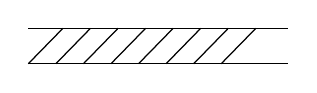
\begin{tikzpicture}[line width=.45pt]
  \draw (0,0) -- (3.3,0) (0,.45) -- (3.3,.45);
  \foreach \x in {0,.35,...,2.8}
    \draw (\x,0) -- ++(.44,.45);
\end{tikzpicture}}\endgroup\par
Две строки между горизонтальными чертами пересечены наклонными штрихами. Последняя запись предположительно читается «супер» и готическая g.}
\end{GelfandAdjacentEvidence}
\begin{GelfandAdjacentEvidence}{GELFAND-P000663}{3}


\underline{Градуировка:} \(\Lambda^p(\mathfrak g')\otimes S^q(\mathfrak g')\)
имеет степень \(p+2q\).

\underline{Дифференциал:} \(d:W(\mathfrak g)\to W(\mathfrak g)\) со свойствами

1) \(d^2=0\), 2) обычным образом действует на [зачёркнута запись] произведение.
\Incomplete{GELFAND-P000663}{cancel-product}{Короткая запись перед «произведение» густо зачёркнута.}
\end{GelfandAdjacentEvidence}
\begin{GelfandAdjacentEvidence}{GELFAND-P000663}{4}


Пусть \(h\in\underset{\substack{\Vert\\\Lambda^1(\mathfrak g')}}{\mathfrak g'}\).
Рассмотрим \(h\otimes1\in W(\mathfrak g)\).
\[
\begin{aligned}
d:\Lambda^1(\mathfrak g')\otimes S^0(\mathfrak g')\to{}&
\Lambda^2(\mathfrak g')\otimes S^0(\mathfrak g')\\
&\oplus\Lambda^0(\mathfrak g')\otimes S^1(\mathfrak g').
\end{aligned}
\]
\[
h\otimes1\ [h\text{? зачёркнуто}]\ \mapsto
\bigl\{(g_1,g_2)\mapsto h([g_1,g_2])\bigr\}\otimes1;\qquad 1\otimes h.
\]
\Unclear{GELFAND-P000663}{cancel-map}{Зачёркнутый знак перед стрелкой похож на h.}
\end{GelfandAdjacentEvidence}
\begin{GelfandAdjacentEvidence}{GELFAND-P000663}{5}

Это продолжается единств. образом до дифф. со св-вами 1) и 2).

\underline{Св-во 2)}.
\[
\xi\in W^k(\mathfrak g),\quad\eta\in W^\ell(\mathfrak g)
\ \Longrightarrow\ d(\xi\cdot\eta)=d\xi\cdot\eta+(-1)^k\xi\cdot d\eta.
\]
На [зачёркнута запись] определяется из условия \(d^2=0\).
\Incomplete{GELFAND-P000663}{cancel-domain}{Запись после «На» зачёркнута косыми штрихами.}
\end{GelfandAdjacentEvidence}
\begin{GelfandAdjacentEvidence}{GELFAND-P000663}{6}

\SourceFigure{GELFAND-P000663}{domain-callout}{%
\par\smallskip
\begingroup\color{black}\GelfandFitDiagram{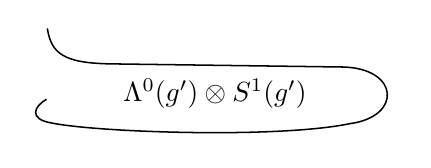
\begin{tikzpicture}[line width=.55pt]
\node at (0,0) {\(\Lambda^0(\mathfrak g')\otimes S^1(\mathfrak g')\)};
\draw (-2.13,.83) .. controls (-2.08,.51) and (-1.92,.39) .. (-1.33,.38)
  -- (1.63,.34) .. controls (2.34,.32) and (2.38,-.29) .. (1.71,-.38)
  .. controls (.78,-.57) and (-1.50,-.49) .. (-2.08,-.37)
  .. controls (-2.37,-.32) and (-2.30,-.16) .. (-2.14,-.07);
\end{tikzpicture}}\endgroup\par
Обведённая вставка соединена с местом после «На».}
\end{GelfandAdjacentEvidence}
\begin{GelfandAdjacentEvidence}{GELFAND-P000663}{7}

\[
d:W^k(\mathfrak g)\to W^{k+1}(\mathfrak g).
\]
\[
d(h\otimes1)=(dh\otimes1)\oplus(1\otimes h),
\]
где \((dh)(g_1,g_2)\overset{\cdot}{=}h([g_1,g_2])\).

\(\overset{\cdot}{=}\) означает \(\overset{\mathrm{def}}{=}\).
\[
(dh)(g_1,\ldots,g_{\ell+1})=
\]
\Unclear{GELFAND-P000663}{bottom-index}{Последний знак индекса больше похож на \(1\), как в показателе \(i+j-1\). Чтение \(\ell+1\) предположительное.}
\end{GelfandAdjacentEvidence}
\begin{GelfandAdjacentEvidence}{GELFAND-P000663}{8}


[Зачёркнута первая сумма: \(\sum(-1)^i h(\ldots)\).]
\Incomplete{GELFAND-P000663}{cancel-bottom}{Видны сумма, знак с показателем i, буква h, скобки и несколько g. Полная запись не устанавливается.}
\end{GelfandAdjacentEvidence}
\begin{GelfandAdjacentEvidence}{GELFAND-P000663}{9}

\[
\sum_{i<j}(-1)^{i+j-1}h([g_i,g_j],g_1,\ldots,\widehat g_i,\ldots,\widehat g_j).
\]
\Unclear{GELFAND-P000663}{bottom-arguments}{После коммутатора первый индекс предположительно \(1\). Над двумя последними \(g\) стоят крышки. В конце виден лишний штрих.}
\end{GelfandAdjacentEvidence}



\Needspace{7\baselineskip}
\begin{GelfandAdjacentEvidence}{GELFAND-P000664}{1}
\SourcePage{GELFAND-P000664}{unlabelled}
\[
dh=\sum a_i h_{i_1}\wedge h_{i_2}
  =\sum a_i(h_{i_1}\otimes1)(h_{i_2}\otimes1).
\]
Дифференц. по Лейбницу.

Появится ненулевой элемент \(\underline{\Lambda^1\otimes S^1}\).

Пусть \(e_1,\ldots,e_n\) --- базис в \(\mathfrak g\), он же базис линейных ф-ий на \(\mathfrak g'\).

\(h^1,\ldots,h^n\) --- дуальный базис в \(\mathfrak g'\).

Тогда
\[
\begingroup\color{black}\GelfandFitDiagram{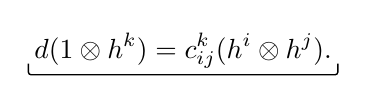
\begin{tikzpicture}[baseline=(structure.base)]
\node[inner sep=2pt] (structure)
  {$\displaystyle d(1\otimes h^k)=c_{ij}^k(h^i\otimes h^j).$};
\draw[line width=.5pt,rounded corners=1pt]
  ([yshift=4pt]structure.south west) -- (structure.south west) --
  (structure.south east) -- ([yshift=4pt]structure.south east);
\end{tikzpicture}}\endgroup
\]

\underline{Осн. теорема:} Гомологии комплекса
\(\underline{\ldots}\to W^k\underline{\xrightarrow{d}}W^{k+1}\to\ldots\)
равны \(0\).

\underline{След. раз:} как она работает в хар. классах.

\underline{А.\,А. Кириллов.} Придумано для счёта гомологий простых компактных групп Ли.

Простая часть: это инвар. формы.

Легко искать симметрические. Кососимметрические?

\(\omega^k\) --- кососимм. инвар. дифф. форма.
\[
\omega^k\in\Lambda^k\otimes S^0+\ldots;\qquad d\omega^k=0.
\]
\Unclear{GELFAND-P000664}{omega-degree}{Верхний индекс \(\omega\) в строке принадлежности наведён. Предположительно это \(k\), как в соседних записях.}
\end{GelfandAdjacentEvidence}
\begin{GelfandAdjacentEvidence}{GELFAND-P000664}{2}

Тогда \(\omega^k\) --- дифф. симм. выраж..

Вывод: кососимметр. [вставлено сверху: инв.] степ. \(k\) столько, сколько симм. степ. \(\frac{k+1}{2}\).
\SourceFigure{GELFAND-P000664}{invariant-callout}{%
\par\smallskip
\begingroup\color{black}\GelfandFitDiagram{\begin{tikzpicture}[line width=.55pt]
\node at (0,.29) {инв.};
\draw (-.64,.49) .. controls (-.75,.18) and (-.57,.09) .. (-.32,.03)
  .. controls (-.14,-.02) and (-.06,-.14) .. (-.08,-.29)
  .. controls (-.01,-.04) and (.21,.07) .. (.42,.09)
  .. controls (.58,.13) and (.67,.27) .. (.72,.43);
\end{tikzpicture}}\endgroup\par
Сокращение «инв.» вставлено сверху между «кососимметр.» и «степ.».}
\end{GelfandAdjacentEvidence}
\begin{GelfandAdjacentEvidence}{GELFAND-P000664}{3}

\[
\text{---''---}\quad 3\qquad \text{---''---}\quad 2.
\]

\underline{Арнольд.}\quad\underline{О работах конца прошлого века о 2-х вопр.}

1) \(y''=F(x,y,y')\) (напр., \(y''=0\)).

Tresse (ученик Софуса Ли) 1896, Acta Math. 1894.

\(y''=0\)\quad графики прямые.
\SourceFigure{GELFAND-P000664}{three-lines}{%
\par\smallskip
\begingroup\color{black}\GelfandFitDiagram{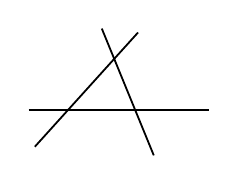
\begin{tikzpicture}[line width=.65pt]
\draw (-1.15,0)--(1.14,0);
\draw (-1.07,-.47)--(.24,.98);
\draw (-.22,1.03)--(.44,-.58);
\end{tikzpicture}}\endgroup\par
Три прямые справа от текста попарно пересекаются, образуя треугольник.}
\end{GelfandAdjacentEvidence}
\begin{GelfandAdjacentEvidence}{GELFAND-P000664}{4}


Есть конфигур. теоремы (Паппа, Дезарга, Паскаля и т.д.).

Можно ли выпрямить реш. общего ур-я?

Линейное меню \(\Longrightarrow\) верны все конфиг. теор. (Дезарга для синусоид).
\Unclear{GELFAND-P000664}{linear-phrase}{Второе слово предположительно читается «меню».}
\end{GelfandAdjacentEvidence}
\begin{GelfandAdjacentEvidence}{GELFAND-P000664}{5}

\Unclear{GELFAND-P000664}{desargues-phrase}{Слово между «Дезарга» и «синусоид» читается предположительно «для».}
\end{GelfandAdjacentEvidence}

\[
y''+a(x)y'+b(x)y=0
\]
прив. диффеом. плоскости \((x,y)\), линейным по \(y\):
\[
\begin{aligned}
x&=f(\tilde x)\\
y&=g(\tilde x)\tilde y
\end{aligned}
\]
Локально приводится к \(y''=0\).


\Needspace{7\baselineskip}
\begin{GelfandAdjacentEvidence}{GELFAND-P000665}{1}
\SourcePage{GELFAND-P000665}{unlabelled}
Рассм. произвольное сем-во.

Инфинитезимальная теория небезызвестна.

\underline{E. Cartan} в 1924–25 г., --- проективная связность ---

--- решения --- геодезич. отн. этой связности.

Проект. связность --- связн. в \(G\)-рассл., где \(G\) --- проект. группа, действ. в кас. пр-ве.

Пр-во линейных элементов \((x,y,y')\).

2) В \(\mathbb R^3\) есть 2 поля напр..
\SourceFigure{GELFAND-P000665}{direction-grid}{%
\par\smallskip
\begingroup\color{black}\GelfandFitDiagram{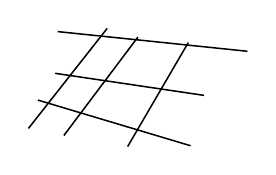
\begin{tikzpicture}[line width=.55pt]
  \draw (-.95,.48) -- (1.46,.23);
  \draw (-.98,-.05) -- (.91,-.33);
  \draw (-1.20,-.39) -- (.74,-.97);
  \draw (-1.32,-.75) -- (-.32,.52);
  \draw (-.87,-.84) -- (.07,.41);
  \draw (-.06,-.98) -- (.71,.34);
\end{tikzpicture}}\endgroup\par
Две семьи по три штриха пересекаются, образуя наклонную сетку.}
\end{GelfandAdjacentEvidence}
\begin{GelfandAdjacentEvidence}{GELFAND-P000665}{2}


Гр. диффеом. \(\mathbb R^3\) действует.

[наведённый знак] К какому виду можно привести?
\Unclear{GELFAND-P000665}{question-prefix}{Отдельный густо наведённый знак перед «К» не установлен.}
\end{GelfandAdjacentEvidence}
\begin{GelfandAdjacentEvidence}{GELFAND-P000665}{3}


\underline{Эти задачи эквивалентны.}

Выбр. 1 напр., спроект. вдоль него на плоскость. Там 2-парам. сем-во и т. д.
\Unclear{GELFAND-P000665}{restriction-word}{После «1 напр.» читается сокращение «спроект.».}
\end{GelfandAdjacentEvidence}
\begin{GelfandAdjacentEvidence}{GELFAND-P000665}{4}


В жизни \underline{Бляшке} занимался.
\Unclear{GELFAND-P000665}{blaschke-phrase}{Слово между «В» и «Бляшке» предположительно читается «жизни».}
\end{GelfandAdjacentEvidence}
\begin{GelfandAdjacentEvidence}{GELFAND-P000665}{5}


В \(\mathbb R^3\) есть контактная структура. (Плоскости, натян. на кас. векторы).

Кривые им. структ. локально проективной прямой.
\Unclear{GELFAND-P000665}{curve-word}{Короткая запись после «Кривые» предположительно читается «им.».}
\end{GelfandAdjacentEvidence}
\begin{GelfandAdjacentEvidence}{GELFAND-P000665}{6}


(из общей теории многомерных расслоений)
\Unclear{GELFAND-P000665}{bundle-adjective}{Прилагательное перед «расслоений» предположительно читается «многомерных».}
\end{GelfandAdjacentEvidence}
\begin{GelfandAdjacentEvidence}{GELFAND-P000665}{7}


На окружности есть много не-эквив. структур лок. проект. пр-ва.
\[
1)\quad\mathbb{RP}^1\qquad
2)\quad S^1\xrightarrow[\text{степ.}~2]{}\mathbb{RP}^1
\]
2) не-эквив. структура.

\underline{Д-во не-эквив.:} просм. вект. поля (инфинитезим. автом. этой структуры).
\Unclear{GELFAND-P000665}{proof-verb}{Сокращение перед «вект. поля» предположительно читается «просм.».}
\end{GelfandAdjacentEvidence}
\begin{GelfandAdjacentEvidence}{GELFAND-P000665}{8}

\[
\text{на }\mathbb{RP}^1\quad
\frac{\partial}{\partial x},\quad
x\frac{\partial}{\partial x},\quad x^2\frac{\partial}{\partial x}.
\]

\underline{Задача:} как [зачёркнута запись] уравнение [зачёркнута запись] в целом локально проективное пр-во?
\Incomplete{GELFAND-P000665}{cancel-first}{Написанное слово между «как» и «уравнение» густо зачёркнуто.}
\end{GelfandAdjacentEvidence}
\begin{GelfandAdjacentEvidence}{GELFAND-P000665}{9}

\Incomplete{GELFAND-P000665}{cancel-second}{Слово после «уравнение» перечёркнуто несколькими штрихами.}
\end{GelfandAdjacentEvidence}
\begin{GelfandAdjacentEvidence}{GELFAND-P000665}{10}

\Unclear{GELFAND-P000665}{question-word}{После зачёркивания читается «в целом локально».}
\end{GelfandAdjacentEvidence}
\begin{GelfandAdjacentEvidence}{GELFAND-P000665}{11}


Примем одну реш. за прямую.
\SourceFigure{GELFAND-P000665}{reference-line}{%
\par\smallskip
\begingroup\color{black}\GelfandFitDiagram{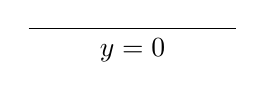
\begin{tikzpicture}[line width=.6pt]
\draw (-1.32,0)--(1.32,0);
\node[below] at (0,0) {\(y=0\)};
\end{tikzpicture}}\endgroup\par
Под прямой справа подписано \(y=0\).}
\end{GelfandAdjacentEvidence}
\begin{GelfandAdjacentEvidence}{GELFAND-P000665}{12}

\[
y''=a(x)y+b(x)p+\ldots
\]
[Справа: члены выс. степ. по \(y'\).]
\Unclear{GELFAND-P000665}{margin-degree}{Первые слова приписки читаются «члены выс. степ.».}
\end{GelfandAdjacentEvidence}
\begin{GelfandAdjacentEvidence}{GELFAND-P000665}{13}

\[
p=y'.
\]

Выпрямляем лин. ур-е. Коорд. \(x\) сопр. с т-ми её проективного простр.
\Unclear{GELFAND-P000665}{coordinate-line}{Сокращение после «с» предположительно читается «т-ми».}
\end{GelfandAdjacentEvidence}

\[
\begin{cases}
\tilde x=f(x),\\
\tilde y=g(x)y.
\end{cases}
\]
(\(f\) уд. ур-ю типа Шварца).


\Needspace{7\baselineskip}
\begin{GelfandAdjacentEvidence}{GELFAND-P000666}{1}
\SourcePage{GELFAND-P000666}{unlabelled}
Отсюда на \(\forall\) реш. возникает проект. структура.

Теперь нач. с квадр. части.
\[
y''=a(x)y^2+b(x)yy'+c(x)y'^2+\ldots
\]
\SourceFigure{GELFAND-P000666}{quadratic-marks}{%
\par\smallskip
\begingroup\color{black}\GelfandFitDiagram{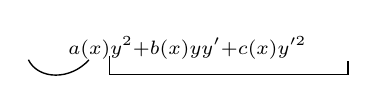
\begin{tikzpicture}[line width=.5pt]
\node at (0,0) {\(\scriptstyle a(x)y^2+b(x)yy'+c(x)y'^2\)};
\draw (-2.02,-.15) .. controls (-1.89,-.41) and (-1.48,-.41) .. (-1.25,-.15);
\draw (-.99,-.10) -- (-.99,-.34) -- (2.04,-.34) -- (2.04,-.16);
\end{tikzpicture}}\endgroup\par
Под первым членом дуга. Скобка под следующими членами до \(c(x)y'^2\).}
\end{GelfandAdjacentEvidence}
\begin{GelfandAdjacentEvidence}{GELFAND-P000666}{2}


Теперь диффеом. плоскости вида:
\[
\begin{cases}
\tilde x=x+yf(x,y),\\
\tilde y=y(1+yg(x,y)).
\end{cases}
\]
Убьём \(b\) и \(c\) этими диффеом..

Остаётся \(a\), опр. с точн. до мульт. постоянной.
\[
\underline{\underline{a(x)(dx)^{5/2}}}\qquad\text{опр. с точн. до мульт. постоянной.}
\]
Это 5/2-форма вдоль решения, опр. с точн. до мульт. конст., зав. от решения.

\underline{Теорема.} Если \(a(x)(dx)^{5/2}\equiv0\), \underline{то ур-е выпрямляемо}.

(в форм. рядах)

Дальнейшие дифф-мы прив. к \(\underline{\underline{y''=y'^2A(x,y,y')}}\).

Рассм. ур-е вида \(\underline{y''=P_3(y')}\) --- многоч. 3-й степени отн. \(y'\).

Этот класс инвар. отн. диффеоморфизмов.

Появл. этих ур-ий открыл \underline{R. Liouville}.
\Unclear{GELFAND-P000666}{liouville-verb}{Глагол перед именем предположительно читается «открыл».}
\end{GelfandAdjacentEvidence}
\begin{GelfandAdjacentEvidence}{GELFAND-P000666}{3}


\underline{Скалярный инвариант.}

Из эт. форма \(\forall\) друг. степ. (в частн. вект. поле).
\[
\begingroup\color{black}\GelfandFitDiagram{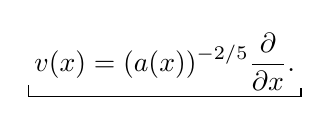
\begin{tikzpicture}[baseline=(field.base)]
\node[inner sep=2pt] (field)
  {$\displaystyle v(x)=(a(x))^{-2/5}\frac{\partial}{\partial x}.$};
\draw[line width=.5pt] ([yshift=4pt]field.south west) -- (field.south west) --
  (field.south east) -- ([yshift=3pt]field.south east);
\end{tikzpicture}}\endgroup
\]
\Unclear{GELFAND-P000666}{from-this}{Начало строки читается предположительно «Из эт.».}
\end{GelfandAdjacentEvidence}
\begin{GelfandAdjacentEvidence}{GELFAND-P000666}{4}


\underline{Скаляр устроим теперь:} хотим, чтобы коммутир. с действ. проект. группы.
\Unclear{GELFAND-P000666}{scalar-clause}{После «хотим» читается «чтобы коммутир.».}
\end{GelfandAdjacentEvidence}

Получим инварианты:

\(I_2,I_3,\ldots\) --- инварианты.

Рассм. 2-струю поля. На 2-струях проект. гр. действ. присоед. представлением.
\[
\begin{gathered}
\underline{I_2=2v''v-v'^2}\\
\underline{I_3=vI_2'}\\
\text{---\quad ---\quad ---}\\
\underline{I_n=vI_{n-1}'}
\end{gathered}
\]
\underline{Гип. Гельфанда:} связано с когомологиями Гельфанда–Фукса.

\underline{Pommaret} занимался дифф. инвариантами.


\Needspace{7\baselineskip}
\begin{GelfandAdjacentEvidence}{GELFAND-P000667}{1}
\SourcePage{GELFAND-P000667}{unlabelled}
\underline{20/IX-76 г.}\quad\underline{Сем. Гельфанда.}

\underline{С.\,П. Новиков.}\quad\underline{Супералгебры в физике.}

[Зачёркнуто: Обз.?] \underline{Обзор Огиевецкого в УФН и обзор Зумино}.
\Unclear{GELFAND-P000667}{cancel-review}{Зачёркнутое начало предположительно читается «Обз.».}
\end{GelfandAdjacentEvidence}
\begin{GelfandAdjacentEvidence}{GELFAND-P000667}{2}

\SourceFigure{GELFAND-P000667}{margin-authors}{%
\par\smallskip
\begingroup\color{black}\GelfandFitDiagram{\begin{tikzpicture}[line width=.55pt]
  \draw (-.10,0) rectangle (.10,1.00);
  \draw (-.18,0) -- (.18,0) (-.18,1.00) -- (.18,1.00);
  \foreach \y in {.02,.15,...,.80}
    \draw (-.10,\y) -- ++(.20,.19);
  \node[anchor=west,inner sep=0] (names) at (.44,.77) {Волков, Акулов};
  \draw[dashed] ([yshift=-1pt]names.south west) -- ([yshift=-1pt]names.south east);
\end{tikzpicture}}\endgroup\par
На правом поле фамилии с прерывистым подчёркиванием. Слева от них узкий заштрихованный знак.}
\end{GelfandAdjacentEvidence}
\begin{GelfandAdjacentEvidence}{GELFAND-P000667}{3}


Супералгебра [Зачёркнуто: Ли?] --- прям. сумма
\(L=L_{\text{чет}}\oplus L_{\text{нечет}}=L_0\oplus L_1\).
\Unclear{GELFAND-P000667}{cancel-super}{Штрихи короткого зачёркнутого слова напоминают «Ли».}
\end{GelfandAdjacentEvidence}
\begin{GelfandAdjacentEvidence}{GELFAND-P000667}{4}


\([a,b]\) опр. структ. градуир. алгебры Ли.
\[
[a,b]=(-1)^{da\cdot db+1}[b,a],\qquad da=\dim a.
\]
\Unclear{GELFAND-P000667}{degree-notation}{В определении \(da\) написано «dim a».}
\end{GelfandAdjacentEvidence}


Тожд. Якоби тоже вып. со знаками.

Пусть \(L_0\) и \(L_1\) влож. в ассоц. алгебру (напр., матриц).

\(L\) --- подалгебра матр. алг., замкн. отн. операции
\[
\begin{aligned}
1)\quad &a,b\in L_0\ \Longrightarrow\ ab-ba=[a,b]\in L_0,\\
2)\quad &a,b\in L_1\ \Longrightarrow\ ab+ba=[a,b]\in L_0.
\end{aligned}
\]


\Needspace{7\baselineskip}
\begin{GelfandAdjacentEvidence}{GELFAND-P000668}{1}
\SourcePage{GELFAND-P000668}{unlabelled}
\[
3)\quad a\in L_0,\ b\in L_1\ \Longrightarrow\ ab-ba=[a,b]\subset L_1.
\]
Или
\[
\begin{gathered}
[a,b]=(-1)^{\varepsilon_1\varepsilon_2+1}[b,a],\\
\varepsilon_1=\operatorname{deg} a,\qquad
\varepsilon_2=\operatorname{deg} b.
\end{gathered}
\]
Впервые рассм. в раб. Гельфанда и Лихтмана конкр. супералгебры.
\[
\mu=0,1,2,3.
\]
Всё в \(\mathbb R^4\) Минковский.
\[
\eta_{\nu,\mu}=\begin{pmatrix}
-1&&&0\\ &1&&\\ &&1&\\0&&&1
\end{pmatrix}\quad\text{--- метрика.}
\]
\underline{пр-во спиноров} --- 4-мерное пр-во
[вставлено сверху: веществ.. Зачёркнуто слово.] (с базисом) \(Q_j\), \(j=1,2,3,4\).
\SourceFigure{GELFAND-P000668}{cancel-complex}{%
\par\smallskip
\begingroup\color{black}\GelfandFitDiagram{\begin{tikzpicture}[line width=.55pt]
\node at (0,.30) {веществ.};
\node at (0,-.02) {\scriptsize [зачёркнуто]};
\draw (-1.21,.53) .. controls (-1.53,.03) and (-.91,-.23) .. (-.44,-.32)
  .. controls (-.21,-.38) and (-.10,-.53) .. (-.11,-.68)
  .. controls (.07,-.48) and (.30,-.31) .. (.72,-.23)
  .. controls (1.11,-.15) and (1.30,.14) .. (1.32,.48);
\end{tikzpicture}}\endgroup\par
«Веществ.» написано в обведённой вставке. Нижнее слово зачёркнуто.}
\end{GelfandAdjacentEvidence}
\begin{GelfandAdjacentEvidence}{GELFAND-P000668}{2}

\SourceFigure{GELFAND-P000668}{basis-callout}{%
\par\smallskip
\begingroup\color{black}\GelfandFitDiagram{\begin{tikzpicture}[line width=.55pt]
\node at (.09,.25) {с базисом};
\draw (-.83,.49) .. controls (-.72,.22) and (-.70,-.06) .. (-.69,-.35)
  .. controls (-.61,-.13) and (-.44,.01) .. (-.22,.01)
  -- (.75,.04) .. controls (.98,.05) and (1.02,.18) .. (1.06,.40);
\end{tikzpicture}}\endgroup\par
Вторая обведённая вставка «с базисом» направлена к началу списка.}
\end{GelfandAdjacentEvidence}
\begin{GelfandAdjacentEvidence}{GELFAND-P000668}{3}

\[
\alpha=\sum\alpha^j Q_j.
\]
Алгебра матриц порожд. матр. \(\gamma_\mu\) (веществ.) --- базис Майорана.
\[
\gamma_\mu\gamma_\nu+\gamma_\nu\gamma_\mu=2\eta_{\nu\mu}.
\qquad(\approx\text{ кватернионы})
\]
Выберем 4 матрицы \(\gamma_\mu\), веществ. и обр. базис Майорана

(см. Ахиезер, Берестецкий).

Положим
\[
\begin{aligned}
\bar Q_j&=Q_j\gamma_0;\\
\bar\alpha&=\alpha\gamma_0.
\end{aligned}
\]
\Unclear{GELFAND-P000668}{spinor-letter}{У буквы \(Q\) виден нижний косой штрих.}
\end{GelfandAdjacentEvidence}
\begin{GelfandAdjacentEvidence}{GELFAND-P000668}{4}


\(L_0\) --- алг. [зачёркнуто: Пуанкаре] трансляций.
\Unclear{GELFAND-P000668}{poincare-cancel}{Слово «Пуанкаре» перечёркнуто перед «трансляций».}
\end{GelfandAdjacentEvidence}
\begin{GelfandAdjacentEvidence}{GELFAND-P000668}{5}


\(L_1\) --- пр-во спиноров.
\[
\begin{aligned}
1)\quad &[L_1,L_0]=0,\\
2)\quad &[L_1,L_1]\text{ --- ?}
\end{aligned}
\]
\[
[\bar Q_i,\bar Q_j]=-2(\gamma^\mu)_{ij}P_\mu.
\]
\(P_\mu\) --- опер. трансляции Пуанкаре, \(\mu\) --- индекс.

Г. \underline{Задача.} расширить алг. Пуанкаре до супералгебры.

\SourceFigure{GELFAND-P000668}{field-figure}{%
\par\smallskip
\begingroup\color{black}\GelfandFitDiagram{\begin{tikzpicture}[line width=.55pt, every node/.style={font=\footnotesize}]
\node[anchor=west,inner sep=0] (fields) at (.86,0) {%
  \(\begin{array}{@{}r@{\ \text{---}\ }l@{}}
  A & \text{скал. поле}\\
  B & \text{псевдоскал. поле}\\
  \psi & \text{скал. поле}\\
  F & \text{---''---}\\
  G & \text{псевдоск. поле}
  \end{array}\)};
\draw (.79,-.20) .. controls (.78,-.37) and (.73,-.47) .. (.66,-.49)
  .. controls (.74,-.52) and (.78,-.66) .. (.79,-.79);
\node[align=center,inner sep=0] at (.27,-.49) {вспом.\\поля};
\draw ([xshift=3pt]fields.north east) -- ([xshift=3pt]fields.south east);
\draw[<-] ([xshift=5pt]fields.east) -- ([xshift=14pt]fields.east);
\node[anchor=west,inner sep=0] at ([xshift=16pt]fields.east) {супермультиплет};
\end{tikzpicture}}\endgroup\par
Слева скобка объединяет \(F,G\). Справа подпись со стрелкой к вертикальной черте вдоль списка.}
\end{GelfandAdjacentEvidence}
\begin{GelfandAdjacentEvidence}{GELFAND-P000668}{6}

\Unclear{GELFAND-P000668}{field-label}{Напротив \(\psi\) также написано «скал. поле».}
\end{GelfandAdjacentEvidence}
\begin{GelfandAdjacentEvidence}{GELFAND-P000668}{7}

\[
\begin{aligned}
L={}&-\tfrac12\bigl((\partial_\nu A)^2+(\partial_\mu B)^2
+i\bar\psi\gamma^\mu\partial_\mu\psi\\
&\qquad +m^2A^2+m^2B^2+im\bar\psi\psi\bigr)\\
&+gmA(A^2+B^2)-g_2^2(A^2+B^2)^2\\
&-ig\,[im\text{? зачёркнуто}]\,\bar\psi(A-\gamma_5B)\psi.
\end{aligned}
\]
\Unclear{GELFAND-P000668}{kinetic}{Перед верхним \(\mu\) после \(\bar\psi\) видны слабые штрихи, предположительно \(\gamma\).}
\end{GelfandAdjacentEvidence}
\begin{GelfandAdjacentEvidence}{GELFAND-P000668}{8}

\Unclear{GELFAND-P000668}{quartic}{У \(g\) две цифры \(2\), сверху и снизу. Дробная черта не различается.}
\end{GelfandAdjacentEvidence}
\begin{GelfandAdjacentEvidence}{GELFAND-P000668}{9}

\Unclear{GELFAND-P000668}{cancel-term}{Зачёркнутые штрихи после \(-ig\) предположительно читаются \(im\).}
\end{GelfandAdjacentEvidence}
\begin{GelfandAdjacentEvidence}{GELFAND-P000668}{10}


[зачёркнуто: (суперсимм. лагранжиан?)]
\Unclear{GELFAND-P000668}{cancel-bottom}{Последнее слово зачёркнутой скобки предположительно читается «лагранжиан».}
\end{GelfandAdjacentEvidence}



\Needspace{7\baselineskip}
\begin{GelfandAdjacentEvidence}{GELFAND-P000669}{1}
\SourcePage{GELFAND-P000669}{unlabelled}
Опер. из \(L_0\) и \(L_1\) действуют на лагранжиан \(L\) (строится предст.)
и он инвариантен.

\underline{Суперсимм. лагранжиан Вейсса-Зумино.}
\[
\begin{aligned}
L={}&-\tfrac12\bigl((\partial_\nu A)^2+(\partial_\mu B)^2
+i\bar\Psi\gamma^\beta\partial_\mu\Psi-F^2-G^2\bigr]\\
&+m(FA+GB-i\bar\Psi\Psi)\\
&+g(FA^2-FB^2+2GAB-i\bar\Psi\Psi A+i\bar\Psi\gamma_5\Psi B).
\end{aligned}
\]
\Unclear{GELFAND-P000669}{lagrangian-index}{У \(\gamma\) верхний индекс \(\beta\), у \(\partial\) нижний \(\mu\).}
\end{GelfandAdjacentEvidence}
\begin{GelfandAdjacentEvidence}{GELFAND-P000669}{2}

\Unclear{GELFAND-P000669}{lagrangian-brackets}{Внешняя открывающая скобка круглая, закрывающая квадратная.}
\end{GelfandAdjacentEvidence}
\begin{GelfandAdjacentEvidence}{GELFAND-P000669}{3}


По \(F\) и \(G\) нет дифф. \(\Rightarrow\) из ур-й Эйлера они исключаются \(\Rightarrow\)

\(\Rightarrow\) предыд. лагран-жиан.

\underline{Действие суперобразующих.}
\Unclear{GELFAND-P000669}{super-generators}{В заголовке читается «суперобразующих».}
\end{GelfandAdjacentEvidence}
\begin{GelfandAdjacentEvidence}{GELFAND-P000669}{4}

\[
L=L_0+L_1.
\]
\[
\alpha\in L_1,\quad\alpha=\sum\alpha_jQ_j,\qquad\bar\alpha=\alpha\gamma_0.
\]
\[
\begin{aligned}
1)\quad&[\bar\alpha,A]=\delta A=i\bar\alpha\Psi;\\
2)\quad&\delta B=[\text{зачёркнуто}]\ i\bar\alpha\gamma_5\Psi;\\
3)\quad&\delta\Psi=\partial_\mu(A-\gamma_5B)\gamma^\mu\alpha+(F+\gamma_5G)\alpha;\\
4)\quad&\delta F=i\bar\alpha\gamma^\mu\partial_\mu\Psi;\\
5)\quad&\delta G=i\bar\alpha\gamma_5\gamma^\mu\partial_\mu\Psi.
\end{aligned}
\]
\Incomplete{GELFAND-P000669}{delta-b-cancel}{Выражение после \(\delta B=\) зачёркнуто. Видны отдельные знаки.}
\end{GelfandAdjacentEvidence}
\begin{GelfandAdjacentEvidence}{GELFAND-P000669}{5}


\underline{\underline{Мигдал (Саша).}}\quad\underline{О калибровочных полях.}

Возникли из попытки описать экспер. данные (о нуклонах).
Они говорят, что нуклоны состоят из \underline{кварков}.
\SourceFigure{GELFAND-P000669}{proton-figure}{%
\par\smallskip
\begingroup\color{black}\GelfandFitDiagram{\begin{tikzpicture}[line width=.55pt]
\node at (-.75,0) {\(p\sim\)};
\draw[rotate=21] (0,0) ellipse (.35 and .29);
\fill (-.015,.17) ellipse (.062 and .057);
\fill (-.145,-.105) ellipse (.058 and .055);
\fill (.15,-.115) ellipse (.056 and .052);
\node[anchor=west] at (.50,0) {(3 кварка)};
\end{tikzpicture}}\endgroup\par
После \(p\sim\) овал с тремя точками и подписью «3 кварка».}
\end{GelfandAdjacentEvidence}
\begin{GelfandAdjacentEvidence}{GELFAND-P000669}{6}

Внутри свободны, а вынуть их невозможно.

[зачёркнуто: Они.] \underline{Кварки видны} --- просвечивание
[вставлено сверху: протона] \(\gamma\)-квантами (как в целлофановом мешке).
\Unclear{GELFAND-P000669}{they-cancel}{Перед «Кварки» зачёркнуто «Они».}
\end{GelfandAdjacentEvidence}
\begin{GelfandAdjacentEvidence}{GELFAND-P000669}{7}

\SourceFigure{GELFAND-P000669}{proton-callout}{%
\par\smallskip
\begingroup\color{black}\GelfandFitDiagram{\begin{tikzpicture}[line width=.55pt]
\node at (0,.26) {протона};
\draw (-.87,.36) .. controls (-.94,.13) and (-.76,.02) .. (-.47,.03)
  .. controls (-.18,.05) and (.01,-.07) .. (.01,-.23)
  .. controls (.04,-.02) and (.25,.03) .. (.58,.04)
  .. controls (.96,.05) and (.96,.50) .. (.59,.52)
  .. controls (.18,.59) and (-.45,.51) .. (-.72,.43);
\end{tikzpicture}}\endgroup\par
Слово «протона» вставлено перед обозначением квантов.}
\end{GelfandAdjacentEvidence}
\begin{GelfandAdjacentEvidence}{GELFAND-P000669}{8}


\underline{В теории силы должны расти с расстояниями!}

[зачёркнуто] По принципу неопр. они не могут слиться.
\Incomplete{GELFAND-P000669}{principle-cancel}{Короткая запись перед «По принципу» зачёркнута.}
\end{GelfandAdjacentEvidence}
\begin{GelfandAdjacentEvidence}{GELFAND-P000669}{9}


\underline{Релятив. инвар.} мешает зад. закон сил (потенциал взаимод. --- вещь релятив. неинвар.).

\underline{Локальность} проверена просвечиванием --- кварки почти точечны.

надо строить лагранжианы.

Такой зак. сил даёт калибр. теория.

\underline{Кварк} --- \underline{матрица}.
\SourceFigure{GELFAND-P000669}{quark-matrix}{%
\par\smallskip
\begingroup\color{black}\GelfandFitDiagram{\begin{tikzpicture}[line width=.5pt, every node/.style={font=\footnotesize,inner sep=1pt}]
\node (quarks) at (0,0) {\(\begin{pmatrix}
p_1&n_1&\lambda_1\\p_2&n_2&\lambda_2\\p_3&n_3&\lambda_3
\end{pmatrix}\)};
\node at (-1.42,.20) {\(G\)};
\draw[->] (-1.20,.52) -- (-1.20,-.09);
\draw (-1.64,-.77)--(-1.47,-.43) (-1.58,-.77)--(-1.41,-.43);
\node[align=center] at (-1.39,-1.16) {\(SU(3)\)\\(цветовая)};
\draw[->] (-.61,-.77)--(.53,-.77);
\draw[->] (.18,-1.49)--(-.05,-.92);
\node at (.62,-1.71) {гр. неизвестна.};
\node[anchor=west,align=left] at (1.11,.02) {гр. \underline{цвета}\\и гр. \underline{запаха}.};
\end{tikzpicture}}\endgroup\par
Слева \(G\) и стрелка вниз, под матрицей стрелка вправо с припиской. Справа указаны группы цвета и запаха.}
\end{GelfandAdjacentEvidence}
\begin{GelfandAdjacentEvidence}{GELFAND-P000669}{10}


Кварков 9 штук.

Силы, не позв. разрушиться, связаны с цветом.

\underline{Цветной гр.} отвеч. [зачёркнуто] гораздо более сильная симм. --- \underline{калибровочная}.
\Incomplete{GELFAND-P000669}{color-cancel}{Отдельный знак после «отвеч.» густо перечёркнут.}
\end{GelfandAdjacentEvidence}


Мезоны постр. из \underline{кварка и антикварка}.


\Needspace{7\baselineskip}
\begin{GelfandAdjacentEvidence}{GELFAND-P000670}{1}
\SourcePage{GELFAND-P000670}{unlabelled}
\underline{18/X-76.}\quad\underline{Сем. Гельфанда.}

[зачёркнуто] \underline{Написать основные понятия и уравнения, которые надо знать.} \underline{И задачи.}
\Incomplete{GELFAND-P000670}{top-cancel}{Длинная запись перед «Написать» густо зачёркнута.}
\end{GelfandAdjacentEvidence}
\begin{GelfandAdjacentEvidence}{GELFAND-P000670}{2}


\underline{\underline{Задача}}: записать \(\mathrm{II}_1\)-факторы через матрицы непр. порядка.
\Unclear{GELFAND-P000670}{factor-type}{Нижний индекс наведён. По контуру читается 1.}
\end{GelfandAdjacentEvidence}
\begin{GelfandAdjacentEvidence}{GELFAND-P000670}{3}


(не сделанная)
\Unclear{GELFAND-P000670}{factor-parenthesis}{Приписка предположительно читается «не сделанная».}
\end{GelfandAdjacentEvidence}
\begin{GelfandAdjacentEvidence}{GELFAND-P000670}{4}


\underline{\underline{И. Бернштейн.}} (\underline{продолжение}).

\underline{Суперпространство} --- неформально: есть 2 группы перем.:
\[
\left\Vert\begin{array}{l}
x_1,\ldots,x_p,\\
\xi_1,\ldots,\xi_q
\end{array}\right.
\]
\underline{Формально}
\[
C^\infty(\mathbb R^p)\otimes\Lambda(\xi_1,\quad,\xi_q)
\]
Элемент:
\[
\sum f_{\alpha_1.\quad\alpha_q}(x)\xi_1^{\alpha_1}\cdots\xi_q^{\alpha_k},
\qquad \alpha_i=0,1.
\]
\Unclear{GELFAND-P000670}{last-exponent}{У последнего \(\xi_q\) показатель записан как \(\alpha_k\). У коэффициента последний индекс \(\alpha_q\).}
\end{GelfandAdjacentEvidence}
\begin{GelfandAdjacentEvidence}{GELFAND-P000670}{5}


Все \(f\) коммутир. с \(\xi\), и
\(\xi_i\xi_j=-\xi_j\xi_i,\ \xi_i^2=0\).

\(\mathbb Z_2\) --- \underline{Градуировка}.\qquad
\underline{Степень} --- сумма \(\alpha_i\bmod 2.\ \Vert\)

\underline{\underline{Другое опред.}}\qquad
[зачёркнуто] \underline{Кольцованное пр-во}.
\Incomplete{GELFAND-P000670}{ringed-cancel}{Перед «Кольцованное» затушёван узкий знак.}
\end{GelfandAdjacentEvidence}
\begin{GelfandAdjacentEvidence}{GELFAND-P000670}{6}


\(\mathbb R^p\) на нём пучок \(\mathcal A_{p,q}\).
\[
U\subset\mathbb R^p\quad\longmapsto\quad
\text{кольцо }C^\infty(U)\otimes\Lambda(\xi_1,\quad,\xi_q)
\]
\(U\subset V\quad\Rightarrow\quad\) есть естеств. отобр. ограничения.

\underline{\underline{Суперобласть.}} Это топологич. пр-во \(U\subset\mathbb R^p\) с тем же пучком
\[
\mathcal U=(U,\mathcal A_{p,q}).
\]
\Unclear{GELFAND-P000670}{sheaf-letter}{Символ повторяется в записи пары и читается как рукописное \(\mathcal A\).}
\end{GelfandAdjacentEvidence}
\begin{GelfandAdjacentEvidence}{GELFAND-P000670}{7}


[Зачёркнуто над заголовком]
\Incomplete{GELFAND-P000670}{example-cancel}{Короткое слово над «Пример» густо зачёркнуто.}
\end{GelfandAdjacentEvidence}
\begin{GelfandAdjacentEvidence}{GELFAND-P000670}{8}


\underline{Пример.} \(u,\xi_1,\xi_2,\qquad 0<u<1\).
\SourceFigure{GELFAND-P000670}{interval}{%
\par\smallskip
\begingroup\color{black}\GelfandFitDiagram{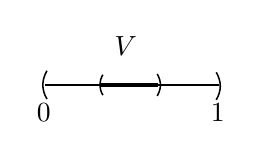
\begin{tikzpicture}[line width=.55pt]
\draw (0,0)--(2.2,0);
\draw (.02,.18) to[bend right=30] (.02,-.18);
\draw (2.17,.16) to[bend left=30] (2.17,-.19);
\draw[line width=1.2pt] (.71,0)--(1.43,0);
\draw (.73,.13) to[bend right=30] (.73,-.13);
\draw (1.42,.14) to[bend left=30] (1.42,-.14);
\node at (1.02,.49) {\(V\)};
\node at (-.02,-.35) {\(0\)};
\node at (2.19,-.35) {\(1\)};
\end{tikzpicture}}\endgroup\par
Внутренний интервал \(V\) отмечен утолщённой линией между скобками.}
\end{GelfandAdjacentEvidence}
\begin{GelfandAdjacentEvidence}{GELFAND-P000670}{9}

функции на \(V=C^\infty(V)\otimes\Lambda(\xi_1,\xi_2)\).
\[
\begin{aligned}
f_{00}(u)+[\text{зачёркнуто}]\,
f_{10}(u)\xi_1+f_{01}\xi_2+f_{11}(u)\xi_1\xi_2.
\end{aligned}
\]
\Incomplete{GELFAND-P000670}{function-cancel}{После \(f_{00}(u)+\) зачёркнута группа знаков.}
\end{GelfandAdjacentEvidence}
\begin{GelfandAdjacentEvidence}{GELFAND-P000670}{10}


\(C^\infty(\widetilde U)\) --- обозначение для пр-ва ф-й на суперобласти \(\widetilde U\).
\[
\begin{gathered}
\Vert\\
C^\infty(U)\otimes\Lambda(\xi_1,\ldots,\xi_q)
\end{gathered}
\]

\underline{Отображение суперобластей} \(\varphi:\widetilde U\longrightarrow\widetilde V\)

это набор объектов: \underline{отображение} \(\varphi':U\to V\)

и \underline{отобр.}
\[
C^\infty(\widetilde V)\longrightarrow C^\infty(\widetilde U)
\]
гом. колец, накрывающий \(\varphi'\) (с единицей) и сохр. \underline{чётность}!!

[зачёркнуто: и если \(V\supset V_0\)?]
\Unclear{GELFAND-P000670}{map-cancel}{В зачёркнутой строке между \(V\) и \(V_0\) различим знак, похожий на \(\supset\).}
\end{GelfandAdjacentEvidence}
\begin{GelfandAdjacentEvidence}{GELFAND-P000670}{11}


\underline{\underline{Пример.}}
\SourceFigure{GELFAND-P000670}{point}{%
\par\smallskip
\begingroup\color{black}\GelfandFitDiagram{\begin{tikzpicture}
\node at (0,0) {\(U\)};
\draw[line width=.65pt] (.95,0) circle (.045);
\node at (1.51,.33) {\(1\)};
\node at (2.07,0) {\(\xi_1,\xi_2\)};
\end{tikzpicture}}\endgroup\par
Рядом с точкой написаны \(U\), \(1\) и \(\xi_1,\xi_2\).}
\end{GelfandAdjacentEvidence}
\begin{GelfandAdjacentEvidence}{GELFAND-P000670}{12}

\underline{\(p=0,\ q=2\).}\qquad Суперобл. размерности \((0,2)\).

Геометрически --- точка. отобр. суперобл. в себя --- эндоморфизм.

Кольца \(\Lambda(\xi_1,\xi_2)\).
\SourceFigure{GELFAND-P000670}{parity-cancel}{%
\par\smallskip
\begingroup\color{black}\GelfandFitDiagram{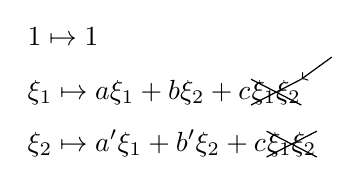
\begin{tikzpicture}[line width=.45pt, every node/.style={inner sep=0}]
\node[anchor=base west] at (0,.73) {\(1\mapsto1\)};
\node[anchor=base west] (first) at (0,.05) {\(\xi_1\mapsto a\xi_1+b\xi_2+c\)};
\node[anchor=base west] (second) at (0,-.61) {\(\xi_2\mapsto a'\xi_1+b'\xi_2+c\)};
\node[anchor=base west] (producta) at (first.base east) {\(\xi_1\xi_2\)};
\node[anchor=base west] (productb) at (second.base east) {\(\xi_1\xi_2\)};
\foreach \term in {producta,productb}{
  \draw (\term.north west) -- (\term.south east)
        (\term.south west) -- (\term.north east);
}
\draw[->] ([xshift=11pt,yshift=8pt]producta.north east) -- (producta.north east);
\end{tikzpicture}}\endgroup\par
Приписка со стрелкой: «нельзя, т. к. сохр. чётность». После последнего плюса перед зачёркнутым произведением читается \(c\). Штрих не установлен.}
\end{GelfandAdjacentEvidence}


\underline{\underline{\(a,b,a',b'\)}} --- любые.


\Needspace{7\baselineskip}
\begin{GelfandAdjacentEvidence}{GELFAND-P000671}{1}
\SourcePage{GELFAND-P000671}{unlabelled}
\underline{Алгебра} \(\Lambda(\xi_1,\xi_2)\) \underline{коммутативна в суперсмысле}.
\[
xy=(-1)^{p(x)p(y)}yx.
\]

\underline{Пример 2.}
\[
\begin{array}{l}
u,\xi_1,\xi_2\\
v,\eta_1,\eta_2
\end{array}
\qquad
\left\Vert\begin{aligned}
v&=u+\xi_1\xi_2\\
\eta_1&=\xi_1\\
\eta_2&=\xi_2.
\end{aligned}\right.
\]
\underline{Задача:} куда переходит \(\sin v\)?

Элемент кольца левого им. вид
\[
f_{00}(u)+f_{10}(u)\xi_1+f_{01}(u)\xi_2+f_{11}(u)\xi_1\xi_2
\]
Элем. 2-го кольца
\[
g_{00}(v)+g_{10}(v)\xi_1+g_{01}(v)\xi_2+g_{11}(v)\xi_1\xi_2
\]
\Unclear{GELFAND-P000671}{second-ring}{В записи 2-го кольца написано \(\xi_1,\xi_2\), как в 1-м.}
\end{GelfandAdjacentEvidence}
\begin{GelfandAdjacentEvidence}{GELFAND-P000671}{2}


\underline{отобр.}
\[
\begin{gathered}
\widetilde U\longrightarrow\widetilde V\\
C^\infty(\widetilde V)\longrightarrow C^\infty(\widetilde U)\\
g_{00}(v)\mapsto g_{00}(u+\xi_1\xi_2)=g_{00}(u)+\xi_1\xi_2g'_{00}(u).
\end{gathered}
\]

\(x=(u_1,\ldots,u_p,\xi_1,\ldots,\xi_q)\) --- система координат.
\[
\frac{\partial}{\partial u_i}f\xi_1^{\alpha_1}\ldots\xi_q^{\alpha_q}
=\frac{\partial f}{\partial u_i}\xi_1^{\alpha_1}\ldots\xi_q^{\alpha_q}
\]

\underline{Теорема Стокса --- ?}

Интеграл суперфункции по суперобласти.

\underline{Аналог в обычном анализе}
\SourceFigure{GELFAND-P000671}{oval-diagram}{%
\par\smallskip
\begingroup\color{black}\GelfandFitDiagram{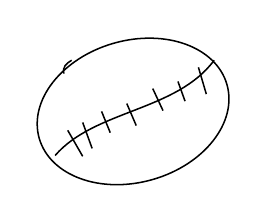
\begin{tikzpicture}[line width=.55pt]
\draw[rotate=16] (0,0) ellipse (1.24 and .90);
\draw (-.99,-.56) .. controls (-.49,.02) and (.55,.00) .. (1.03,.65);
\draw (-.83,-.24)--(-.64,-.57) (-.64,-.14)--(-.52,-.47)
      (-.40,.00)--(-.29,-.27) (-.08,.10)--(.04,-.18)
      (.25,.29)--(.38,.01) (.57,.38)--(.66,.13)
      (.83,.56)--(.93,.22);
\draw (-.88,.48) .. controls (-.90,.56) and (-.85,.61) .. (-.78,.65);
\end{tikzpicture}}\endgroup\par
Внутри овала восходящая кривая и семь видимых поперечных штрихов. Короткий штрих примыкает к контуру слева вверху.}
\end{GelfandAdjacentEvidence}
\begin{GelfandAdjacentEvidence}{GELFAND-P000671}{3}


струи в окр. подмногообразия.
\Unclear{GELFAND-P000671}{middle-phrase}{Первые слова читаются «струи в окр.». Начало слова «подмногообразия» наведено.}
\end{GelfandAdjacentEvidence}
\begin{GelfandAdjacentEvidence}{GELFAND-P000671}{4}


Интеграл для ф-й на мн-зии с границей неинвар. отн. замен переменных.

Отличие: здесь интегрировать формы нельзя. Можно плотности (при замене коорд. умн. на \underline{Березиниан}).

\underline{\underline{Что интегр. по границе?}}

\(\underline{\underline{U,\partial U}}.\)\quad
\(f=0\), где \(f\in C^\infty(U)\) --- \underline{суперфункция}.

\underline{Замкн. суперобласть.}\quad \(\underline{\underline{u,\xi_1,\xi_2}}\)
\SourceFigure{GELFAND-P000671}{boundary-arrow}{%
\par\smallskip
\begingroup\color{black}\GelfandFitDiagram{\begin{tikzpicture}[line width=.5pt]
\node at (.94,.44) {\(\underline{\underline{U,\partial U}}\)};
\node[anchor=west] at (-.53,-.32) {\scriptsize замкн. обл. с гладк. гр. \(\partial U\)};
\draw[->] (-.27,-.05)--(.22,.42);
\end{tikzpicture}}\endgroup\par
Стрелка направлена от приписки к \(U,\partial U\).}
\end{GelfandAdjacentEvidence}
\begin{GelfandAdjacentEvidence}{GELFAND-P000671}{5}


На \(\partial U\) есть структ. [вставлено сверху: под] супермн-зия.
\SourceFigure{GELFAND-P000671}{lower-supermanifold}{%
\par\smallskip
\begingroup\color{black}\GelfandFitDiagram{\begin{tikzpicture}[line width=.5pt]
\node (word) at (0,0) {\underline{\underline{супермн-зия}}};
\node at (0,.57) {\scriptsize под};
\draw (-.31,.62) -- (-.04,.17) -- (.33,.49);
\end{tikzpicture}}\endgroup\par
Вставка «под» направлена к месту после «супер». Окончание сокращения читается предположительно.}
\end{GelfandAdjacentEvidence}
\begin{GelfandAdjacentEvidence}{GELFAND-P000671}{6}


(чётным \underline{ур-ем} [зачёркнуто: это?] \underline{выделяется})
\Unclear{GELFAND-P000671}{lower-cancellation}{Зачёркнутое слово предположительно читается «это».}
\end{GelfandAdjacentEvidence}
\begin{GelfandAdjacentEvidence}{GELFAND-P000671}{7}


\(\underline{\underline{[0,\infty)}}\qquad \underline{\underline{u,\xi_1,\xi_2.}}\)

Разные суперобласти
\[
\begin{aligned}
1.\quad &u=0\\
2.\quad &u+c\xi_1\xi_2=0
\end{aligned}
\]
\SourceFigure{GELFAND-P000671}{bottom-diagram}{%
\par\smallskip
\begingroup\color{black}\GelfandFitDiagram{\begin{tikzpicture}[line width=.65pt]
\draw (-.40,0)--(-.19,1.14)--(.50,1.16)--(.25,.02)--cycle;
\draw[line width=1.0pt] (-.10,.02)--(.13,1.15);
\draw[line width=1.35pt] (-.02,.02)--(.23,1.10);
\node[anchor=west] at (.65,.62) {\underline{чётное ур-е}};
\end{tikzpicture}}\endgroup\par
Узкий наклонный четырёхугольник с густыми продольными штрихами. Надпись справа относится к рисунку.}
\end{GelfandAdjacentEvidence}



\Needspace{7\baselineskip}
\begin{GelfandAdjacentEvidence}{GELFAND-P000672}{1}
\SourcePage{GELFAND-P000672}{unlabelled}
\underline{\underline{Подмн-зие:}} \underline{в кольце выб. идеал ф-и.}

Граница --- \underline{чётная}.

\(C^\infty(\widetilde U)\)\qquad Граница --- \underline{ур-е}
\(\underline{\underline{f(\widetilde U)=0}}\)
\[
\int \text{финитной ф-и}=\int f_{11\ldots1}\,du_1\ldots du_p
\]

\underline{Для замкн. областей иначе.}

Пусть полупр-во \(\underline{\underline{u_1\ge0}}\)

Тогда интегр. зад. такой же ф-лой.

Он сохр., если перех. в себя как супермн-зие.

\(u_1^2+u_2^2\le1\)
\SourceFigure{GELFAND-P000672}{disk}{%
\par\smallskip
\begingroup\color{black}\GelfandFitDiagram{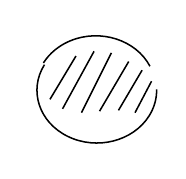
\begin{tikzpicture}[line width=.55pt]
\draw (.68,.30) arc (25:151:.76 and .67);
\draw (-.66,.32) arc (151:361:.76 and .67);
\draw (-.59,-.12)--(-.26,.43) (-.43,-.24)--(-.03,.49)
      (-.19,-.29)--(.19,.47) (.04,-.27)--(.41,.36)
      (.28,-.26)--(.58,.25) (.49,-.29)--(.70,.11);
\end{tikzpicture}}\endgroup\par
Внутри круга наклонные штрихи.}
\end{GelfandAdjacentEvidence}
\begin{GelfandAdjacentEvidence}{GELFAND-P000672}{2}

\[
\begin{gathered}
u_1^2+u_2^2-1=0\quad(1)\quad\text{--- 2 границы}\\
u_1^2+u_2^2-1-\xi_1\xi_2=0\quad(2)
\end{gathered}
\]
Интеграл по обл. с границей (2).
\[
\int[f_{00}(u)+f_{01}(\ )\xi_1+\ldots]
\]
\Unclear{GELFAND-P000672}{integrand-subscript}{После \(f_{01}\) оставлены пустые скобки, затем написано \(\xi_1\).}
\end{GelfandAdjacentEvidence}
\begin{GelfandAdjacentEvidence}{GELFAND-P000672}{3}


\underline{Грубо}
\[
\int\xi_1\xi_2\,d\xi_1\,d\xi_2=1
\]

--- Для обычной границы ---
\[
\int_{u_1^2+u_2^2<1}f_{11}(u)\,du_1du_2
\]

\underline{Проверка инвариантности} --- надо, чтобы ур-е гран. ост. старым.

Если граница \(\underline{u_1^2+u_2^2-1-\xi_1\xi_2=0}\)

надо сделать зам. пер., чтобы гран. перешла в нормальную
\[
\underline{\left(u_1-\tfrac12\xi_1\xi_2\right)^2+u_2^2-1=0.}
\]
\Unclear{GELFAND-P000672}{shifted-circle}{В скобках после \(u_1\) записано \(-\frac12\xi_1\xi_2\).}
\end{GelfandAdjacentEvidence}
\begin{GelfandAdjacentEvidence}{GELFAND-P000672}{4}


[зачёркнуто: \(u=0\)?]
\Unclear{GELFAND-P000672}{upper-cancellation}{Над отрезком предположительно зачёркнуто \(u=0\).}
\end{GelfandAdjacentEvidence}
\begin{GelfandAdjacentEvidence}{GELFAND-P000672}{5}


\SourceFigure{GELFAND-P000672}{half-line}{%
\par\smallskip
\begingroup\color{black}\GelfandFitDiagram{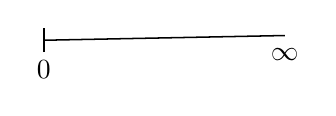
\begin{tikzpicture}[line width=.55pt]
\draw (0,0)--(3.06,.06);
\draw (0,-.15)--(0,.15);
\node[below] at (0,-.13) {\(0\)};
\node[below] at (3.06,.02) {\(\infty\)};
\end{tikzpicture}}\endgroup\par
У левого конца штрих и подпись \(0\), у правого \(\infty\).}
\end{GelfandAdjacentEvidence}
\begin{GelfandAdjacentEvidence}{GELFAND-P000672}{6}

\[
\int_0^\infty f_{11}(u)\,du\qquad u,\xi_1,\xi_2
\]
гран. \(u=0\).

\(\underline{v=u+u\xi_1\xi_2.}\)

Будет граница \(\underline{\underline{v=0}}\)
\[
\begin{aligned}
\int_0^\infty g_{11}(v)\,dv
&=\int_0^\infty g_{11}(u+u\xi_1\xi_2)\,dv\\
&=\int_0^\infty g_{11}(u)\,dv
  +\int_0^\infty g'_{11}(u)u\xi_1\xi_2\,dv
\end{aligned}
\]
\Unclear{GELFAND-P000672}{integral-differentials}{Дифференциал в третьем интеграле похож на \(dv\).}
\end{GelfandAdjacentEvidence}
\begin{GelfandAdjacentEvidence}{GELFAND-P000672}{7}


\SourceFigure{GELFAND-P000672}{integral-sketch}{%
\par\smallskip
\begingroup\color{black}\GelfandFitDiagram{
\begin{tikzpicture}[line width=.55pt]
\draw (-.35,.91) .. controls (-.04,.22) and (.55,-.05) .. (1.15,-.45);
\draw (-.36,.82) .. controls (-.57,.52) and (-1.10,-.03) .. (-1.07,-.18)
  .. controls (-.95,-.22) and (-.56,.43) .. (-.29,.62);
\draw (-.26,.62) .. controls (-.59,.16) and (-.98,-.25) .. (-.88,-.32)
  .. controls (-.73,-.32) and (-.52,.02) .. (-.34,.18);
\draw (-.49,-.11) .. controls (.22,.77) and (.48,.73) .. (.27,.21)
  .. controls (.06,-.16) and (-.48,-.52) .. (-.42,-.58)
  .. controls (-.22,-.66) and (.49,.12) .. (.71,.18)
  .. controls (1.04,.26) and (.68,-.40) .. (.21,-.79);
\end{tikzpicture}}\endgroup\par
Открытая нисходящая кривая с косыми и петлеобразными штрихами. Их соединения различимы не везде.}
\end{GelfandAdjacentEvidence}
\begin{GelfandAdjacentEvidence}{GELFAND-P000672}{8}

\[
\frac{Dv}{Du}
\]
\underline{Интеграл по обл. с границей ---}

\underline{--- Бернштейн и Лейтес}

[зачёркнуто]
\Incomplete{GELFAND-P000672}{lower-cancellation}{Слово перед «Есть раб.» густо перечёркнуто.}
\end{GelfandAdjacentEvidence}
\begin{GelfandAdjacentEvidence}{GELFAND-P000672}{9}


Есть раб. \underline{Березина} и Маринова (?)
\Unclear{GELFAND-P000672}{marinov}{Фамилия предположительно читается «Маринова». В рукописи стоит вопросительный знак.}
\end{GelfandAdjacentEvidence}


\underline{классич. мех. в Ферми и Бозе --- переменных}

\underline{\underline{Задача}}: теор. Стокса для круга \(u_1^2+u_2^2+c\xi_1\xi_2-1=0\).


\Needspace{7\baselineskip}
\begin{GelfandAdjacentEvidence}{GELFAND-P000673}{1}
\SourcePage{GELFAND-P000673}{unlabelled}
\underline{Конспект предыдущих супердокладов И. Бернштейна}

\uline{(по тетради И. Дорфман)}
\Unclear{GELFAND-P000673}{notebook-author}{Имя в скобках предположительно читается «И. Дорфман».}
\end{GelfandAdjacentEvidence}
\begin{GelfandAdjacentEvidence}{GELFAND-P000673}{2}


\underline{Опред.} \underline{Суперкольцо}
\[
A=\underset{\substack{\vert\\\text{чётн}}}{A_0}\oplus
  \underset{\substack{\vert\\\text{нечётн}}}{A_1}
\qquad
\begin{aligned}
 A_0A_0&\subset A_0\\
 A_0A_1&\subset A_1\\
 A_1A_0&\subset A_1\\
 A_1A_1&\subset A_0.
\end{aligned}
\]

Оно наз. \underline{коммутативным}, если
\(\underline{ab=ba(-1)^{\deg a\cdot\deg b}}\)

\underline{Линейная алгебра.}
\Incomplete{GELFAND-P000673}{cancelled-glyph}{Зачёркнутый знак перед скобкой.}
\end{GelfandAdjacentEvidence}
\begin{GelfandAdjacentEvidence}{GELFAND-P000673}{3}

[Над коммут. суперкольцом рассмотрим
\Incomplete{GELFAND-P000673}{cancelled-word-one}{Зачёркнутое слово после «рассмотрим».}
\end{GelfandAdjacentEvidence}
\begin{GelfandAdjacentEvidence}{GELFAND-P000673}{4}

люб. \(A\)-модуль \(A^n\) и его
\Incomplete{GELFAND-P000673}{cancelled-word-two}{Зачёркнутое слово после «его».}
\end{GelfandAdjacentEvidence}
\begin{GelfandAdjacentEvidence}{GELFAND-P000673}{5}

эндоморфизм, задаваемый блочной матрицей]
\[
[A=]\begin{pmatrix}A_{11}&A_{12}\\ A_{21}&A_{22}\end{pmatrix}
\qquad
\det A\underset{\mathrm{def}}{=}
\det A_{11}^{-1}\det(A_{22}-A_{21}A_{11}^{-1}A_{12})
\]
\Unclear{GELFAND-P000673}{determinant-reciprocal}{Слабый верхний индекс у первого \(A_{11}\) читается как \(-1\).}
\end{GelfandAdjacentEvidence}
\begin{GelfandAdjacentEvidence}{GELFAND-P000673}{6}

\[
\begin{gathered}
\operatorname{str}A=\operatorname{tr}A_{11}-\operatorname{tr}A_{22}.\\
(\text{суперслед})
\end{gathered}
\]

\underline{Свойства:}
\[
\begin{gathered}
\det XY=\det X\cdot\det Y.\\
\det X=\exp\operatorname{str}\ln X
\end{gathered}
\]
\Unclear{GELFAND-P000673}{logarithm-tail}{После \(X\) тёмный штрих ниже строки. Возможно, запятая или зачёркнутый знак.}
\end{GelfandAdjacentEvidence}
\begin{GelfandAdjacentEvidence}{GELFAND-P000673}{7}

\[
\begin{gathered}
\operatorname{str}(XY)=\operatorname{str}(YX)\\
\begin{pmatrix}A&B\\ C&D\end{pmatrix}^{*}
=\begin{pmatrix}A^{*}&C^{*}\\ -B^{*}&D^{*}\end{pmatrix}
\end{gathered}
\]

\underline{Суперанализ.}

Рассм.
\[
\sum f_{i_1\quad i_k}(x_1,\mathord{-},x_p)\,
\xi_1^{i_1}\ldots\xi_k^{i_k}
\]
\Unclear{GELFAND-P000673}{expansion-mark}{Между запятыми после \(x_1\) стоит слабый короткий штрих.}
\end{GelfandAdjacentEvidence}
\begin{GelfandAdjacentEvidence}{GELFAND-P000673}{8}


Правила диффер.
\[
\begin{gathered}
\frac{\partial}{\partial\xi_1}(\xi_1\xi_2)=\xi_2,\qquad
\frac{\partial}{\partial\xi_2}(\xi_1\xi_2)=-\xi_1,\\
\frac{\partial}{\partial\xi_1}\xi_2=0,\qquad
\frac{\partial}{\partial\xi_1}\xi_1=1,\qquad
\frac{\partial}{\partial\xi_1}1=0.
\end{gathered}
\]

\noindent\rule{12mm}{.45pt}\enspace\(\cdot\)\enspace\rule{14mm}{.45pt}

Рассм. блочные матрицы \(\begin{pmatrix}A&B\\ C&D\end{pmatrix}\)
\[
\begin{aligned}
A&=A_{\bar{0}}\oplus A_{\bar{1}}\\
\mathbb Z/2\mathbb Z&\text{ --- град.}\\
\bar{0},\bar{1}&\text{ --- элем.}\\
p(a)&\text{ --- чётность}
\end{aligned}
\qquad
\begin{aligned}
\text{элем. }A,D&\in A_{\bar{0}}\\
\text{элем. }B,C&\in A_{\bar{1}}
\end{aligned}
\]
\[
\begin{gathered}
\operatorname{Ber}J=(\det D)^{-1}\cdot\det(A-BD^{-1}C)\in A_{\bar{0}}\\
(\text{березиниан})
\end{gathered}
\]

\underline{У-тв}
\[
\begin{gathered}
\operatorname{Ber}J_1J_2=\operatorname{Ber}J_1\cdot\operatorname{Ber}J_2.\\
\operatorname{str}J=\operatorname{tr}A-\operatorname{tr}D
\end{gathered}
\]
\underline{У-тв.}
\[
\operatorname{str}(J_1J_2)=\operatorname{str}(J_2J_1).
\]

\noindent\rule{11mm}{.45pt}\enspace\(\cdot\)\enspace\rule{15mm}{.45pt}

В \(\mathbb R^p\) рассм. \(C^\infty(\mathbb R^p)\otimes\Lambda(\xi_1,\mathord{\text{---}},\xi_q)\)
\SourceFigure{GELFAND-P000673}{exterior-arrow}{%
\par\smallskip
\begingroup\color{black}\GelfandFitDiagram{\begin{tikzpicture}[line width=.5pt]
\node[anchor=west,inner sep=0pt] at (0,.65)
  {\(\Lambda(\xi_1,\mathord{\text{---}},\xi_q)\)};
\node[anchor=west,inner sep=0pt] at (.50,0) {внешняя алг.};
\draw[->] (.68,.15)--(.78,.43);
\end{tikzpicture}}\endgroup\par
Стрелка от надписи подходит снизу к запятой после \(\xi_1\).}
\end{GelfandAdjacentEvidence}


\(p(\xi_i)=1,\qquad \xi_i\xi_j=-\xi_j\xi_i.\)


\Needspace{7\baselineskip}
\begin{GelfandAdjacentEvidence}{GELFAND-P000674}{1}
\SourcePage{GELFAND-P000674}{unlabelled}
\[
\Lambda(\xi_1,\ldots,\xi_q)\ni\xi_1^{\alpha_1}\cdots\xi_q^{\alpha_q},
\qquad \alpha_i=0,1.
\]
\[
f=\sum f_{\alpha_1\alpha_2\ldots\alpha_q}\,
     \xi_1^{\alpha_1}\cdots\xi_q^{\alpha_q}.
\]

\underline{Опр.}
\[
\mathbb R^{p,q}=
\left(\mathbb R^p,C^\infty(\mathbb R^p)\otimes\Lambda(\xi_1,\ldots,\xi_q)\right)
\]
--- суперпр-во разм. \((p,q)\).

\underline{Опр.}
\[
U=\left(u,\underbrace{C^\infty(u)\otimes\Lambda(\xi_1,\ldots,\xi_q)}
                        _{(\mathrm{def})\, C^\infty(U)}\right)
\]
\uwave{суперобласть.}

(кольцованное пр-во!)

--- кольцо ф-й на обл.
\Unclear{GELFAND-P000674}{upper-ring-abbreviation}{Сокращение после «на» предположительно читается «обл.».}
\end{GelfandAdjacentEvidence}
\begin{GelfandAdjacentEvidence}{GELFAND-P000674}{2}

\SourceFigure{GELFAND-P000674}{ring-definition-callout}{
\par\smallskip
\begingroup\color{black}\GelfandFitDiagram{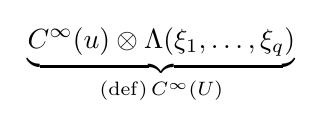
\begin{tikzpicture}
\node[inner sep=0pt] {\(\underbrace{C^\infty(u)\otimes\Lambda(\xi_1,\ldots,\xi_q)}
                              _{(\mathrm{def})\,C^\infty(U)}\)};
\end{tikzpicture}}\endgroup\par
Скобка под тензорным произведением указывает на \((\mathrm{def})\, C^\infty(U)\).}
\end{GelfandAdjacentEvidence}
\begin{GelfandAdjacentEvidence}{GELFAND-P000674}{3}


отобр. \(\widetilde{\psi}:U\to V\)
\Unclear{GELFAND-P000674}{upper-morphism-letter}{Отдельный знак перед тире не разобран.}
\end{GelfandAdjacentEvidence}
\begin{GelfandAdjacentEvidence}{GELFAND-P000674}{4}

--- морфизм кольцев. пр-в ---
это отобр.
\Incomplete{GELFAND-P000674}{upper-map-cancellation}{Перечёркнутая запись перед \(\psi\).}
\end{GelfandAdjacentEvidence}
\begin{GelfandAdjacentEvidence}{GELFAND-P000674}{5}

\[
\psi:C^\infty(V)\to C^\infty(U).
\]
\Unclear{GELFAND-P000674}{pullback-rings}{Аргументы в кольцах функций переданы как \(V\) и \(U\). Регистр букв в рукописи различается слабо.}
\end{GelfandAdjacentEvidence}
\begin{GelfandAdjacentEvidence}{GELFAND-P000674}{6}


\underline{Коорд. запись.} Пусть в пр-ве \(U\) выбр. набор
\[
(u_1,\ldots,u_p,\xi_1,\ldots,\xi_q)
\]
\hspace*{2em}--- \textquotedbl{} --- \(V\) --- \textquotedbl{} ---
\((v_1,\ldots,v_m,\eta_1,\ldots,\eta_n)\).

Оказ., что для задания отобр. \(\psi:U\to V\)
\Incomplete{GELFAND-P000674}{middle-map-cancellation}{Зачёркнутое слово после \(U\to V\).}
\end{GelfandAdjacentEvidence}
\begin{GelfandAdjacentEvidence}{GELFAND-P000674}{7}

дост. задать
\[
v_1^*,\ldots,v_m^*,\eta_1^*,\ldots,\eta_n^*.
\]

\underline{Пример.}
\[
\begin{aligned}
v&=u+\xi_1\xi_2\\
\eta_1&=u\xi_1\\
\eta_2&=\xi_2.
\end{aligned}
\]
\underline{Задача.} Как выглядит \(\sin v\)?

\underline{Утв.}
\[
\frac{\partial}{\partial u_i}(f\xi^\alpha)
=\frac{\partial f}{\partial u_i}\cdot\xi^\alpha,
\]
\[
\begin{aligned}
\frac{\partial}{\partial\xi_j}
  (f\xi_1^{\alpha_1}\cdots\xi_q^{\alpha_q})
&=\alpha_j(-1)^{\alpha_1+\ldots+\alpha_{j-1}}\,
  f\xi_1^{\alpha_1}\cdots\widehat{\xi}_j^{\alpha_j}\cdots\xi_q^{\alpha_q}.
\end{aligned}
\]
\Unclear{GELFAND-P000674}{odd-derivative-omission}{Над \(\xi_j\) стоит знак пропуска, а \(\alpha_j\) остаётся справа вверху. Последний индекс \(q\) наведён.}
\end{GelfandAdjacentEvidence}


\noindent\rule{23mm}{.45pt}\enspace\(\cdot\)\enspace\rule{17mm}{.45pt}

Пусть \(U\) --- суперобласть
\[
\begin{aligned}
x&=(u,\xi)\\
y&=(v,\eta)
\end{aligned}
\]
\[
J=(J_{ij}),\qquad J_{ij}=\frac{\partial y_j}{\partial x_i}.
\]
\[
\operatorname{Ber}J\underset{\mathrm{def}}{=}D(y)/D(x).
\]

\underline{Опред.} \(U\), \(x=(u,\xi)\).

Выраж. \(\rho=fD(x)\) наз. \uwave{формой объема}.
\[
fD(x)=f\bigl(D(x)/D(y)\bigr)\cdot D(y).
\]

\underline{Определение.}
\[
\int_u fD(x)\underset{\mathrm{def}}{=}
\int_u f_{11\ldots1}(u)\,du_1\ldots du_p
\]
(интеграл формы объема)

\underline{Теорема (березин)} Это выраж. не зависит от системы координат.

Здесь интеграл от финитной ф-и берётся.


\Needspace{7\baselineskip}
\begin{GelfandAdjacentEvidence}{GELFAND-P000675}{1}
\SourcePage{GELFAND-P000675}{unlabelled}
\underline{25/X-76.}\qquad \underline{Сем. Гельфанда.}

\underline{Гельфанд.}

\underline{Что такое связность?} (для 1-курсников и Полякова).

--- см. Номидзу; Стернберг; Бишоп и Криттенден; Ландау и Лифшиц.

\uwave{Попов.}

\underline{Работа основоположников} (Янг, Миллс --- перевод в сб. «Элем. частицы и компенсирующие поля»).

Рассмотрим ур-е Дирака

{\small без массы}
\SourceFigure{GELFAND-P000675}{dirac-grouping}{%
\par\smallskip
\begingroup\color{black}\GelfandFitDiagram{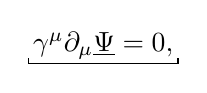
\begin{tikzpicture}[baseline=(eq.base),line width=.45pt]
\node[inner sep=1.5pt] (eq) {\(\gamma^\mu\partial_\mu\underline{\Psi}=0,\)};
\draw ([yshift=2pt]eq.south west)--(eq.south west)--
      (eq.south east)--([yshift=2pt]eq.south east);
\end{tikzpicture}}\endgroup}
\end{GelfandAdjacentEvidence}
\begin{GelfandAdjacentEvidence}{GELFAND-P000675}{2}

\(\Psi=(\Psi_\alpha)\) --- 4-комп. обыкн. спинор.

Ур-я Янга-Миллса:
\[
\underline{\partial_\nu F_a^{\mu\nu}+f^b_{ac}F_b^{\mu\nu}A_\nu^c=0},
\]
\Unclear{GELFAND-P000675}{upper-ym-constant}{Густо наведённые индексы коэффициента предположительно читаются \(f^b_{ac}\).}
\end{GelfandAdjacentEvidence}
\begin{GelfandAdjacentEvidence}{GELFAND-P000675}{3}

где
\[
F_{\mu\nu}^a=\partial_\mu A_\nu^a-\partial_\nu A_\mu^a
+\tfrac12 f_{bc}^a(A_\mu^b A_\nu^c-A_\nu^b A_\mu^c)
\]
на \(\mathbb R^4\) рассм. метрика Минковского \(g_{\mu\nu},\quad A_\mu^\alpha,\quad a=1,\ldots,\dim G\)
\Unclear{GELFAND-P000675}{potential-index}{При \(A_\mu\) написано \(\alpha\), а в следующем перечислении --- \(a\).}
\end{GelfandAdjacentEvidence}
\begin{GelfandAdjacentEvidence}{GELFAND-P000675}{4}


(\(G\) --- нек-рая группа; счит. обычно полупростой).

опуск. индексов в ур-и с пом.
\[
K_{ab}=f_{ac}^d f_{bd}^c,
\]
где \(f_{ac}^d\) --- структ. пост. алгебры Ли группы.

\noindent\rule{9mm}{.45pt}\enspace\(\cdot\)\enspace\rule{12mm}{.45pt}

\underline{\underline{Г.}} О кварках см. ст. \underline{Зельдовича} в УФН \uwave{«Кварки для пешеходов»}.

\noindent\rule{9mm}{.45pt}\enspace\(\cdot\)\enspace\rule{12mm}{.45pt}

Ур-я Янга-Миллса опис. кварки.

\(\mu,\nu=1,\ldots,4\);
\Incomplete{GELFAND-P000675}{middle-cancellation}{Зачёркнутая запись перед \(F_a^{\mu\nu}\).}
\end{GelfandAdjacentEvidence}
\begin{GelfandAdjacentEvidence}{GELFAND-P000675}{5}

\(F_a^{\mu\nu}\) --- тензор со знач. в алгебре Ли.

\(A\) --- аналог вект. потенциала
\[
\partial_\nu=\partial/\partial x^\nu.
\]
\(F\) --- аналог тензора напр.

\underline{Пример.}

Для \(G=U(1)\) получаются ур-я электро-динамики.

\underline{Ур-я:}
\[
\left.
\begin{aligned}
\partial_\mu F^{\mu\nu}&=0\\
F^{\mu\nu}&\underset{\mathrm{def}}{=}\partial_\mu A_\nu-\partial_\nu A_\mu
\end{aligned}
\right\Vert
\]
Получ. ур-я Максвелла.

\noindent\rule{10mm}{.45pt}\enspace\(\cdot\)\enspace\rule{12mm}{.45pt}

\underline{Калибровочные преобразования.}

\underline{В эл. и магн. поле:}
\[
\begin{pmatrix}
0&H_{12}&H_{13}&E_1\\
-H_{12}&0&H_{23}&E_2\\
-H_{13}&-H_{23}&0&E_3\\
-E_1&-E_2&-E_3&0
\end{pmatrix}
=F^{\mu\nu};
\]
\underline{2-форма}
\Unclear{GELFAND-P000675}{field-diagonal}{Третья диагональная запись наведена и читается как ноль.}
\end{GelfandAdjacentEvidence}
\begin{GelfandAdjacentEvidence}{GELFAND-P000675}{6}


\underline{Ур-я Максвелла:}
\[
F^{\mu\nu}=\frac{\partial}{\partial x^\mu}A_\nu
           -\frac{\partial}{\partial x^\nu}A_\mu.
\]
--- \underline{тензор}
\Incomplete{GELFAND-P000675}{lower-tensor-cancellation}{Зачёркнутая запись после «тензор».}
\end{GelfandAdjacentEvidence}
\begin{GelfandAdjacentEvidence}{GELFAND-P000675}{7}

\underline{2-го пор.}

Преобразования \(A\), не меняющие \(F\), наз. градиентными преобразованиями.
\[
A_\mu\to A_\mu+\partial_\mu\alpha
\]
\SourceFigure{GELFAND-P000675}{lower-gradient-cancellation}{%
\par\smallskip
\begingroup\color{black}\GelfandFitDiagram{\begin{tikzpicture}[line width=.5pt]
\node[inner sep=2pt] (new) at (0,0) {градиентными};
\node[inner sep=0pt] (old) at (0,-.65) {\sout{калибр.}};
\draw (new.north west)--(new.north east)
  to[out=0,in=0] (new.south east)
  --([xshift=6pt]new.south west) to[out=180,in=45] (old.west);
\draw ([yshift=-3pt]new.north west)--(old.west);
\end{tikzpicture}}\endgroup\par
Вставка «градиентными» обведена, от обводки идёт указатель к зачёркнутому сокращению, предположительно «калибр.».}
\end{GelfandAdjacentEvidence}



\Needspace{7\baselineskip}
\begin{GelfandAdjacentEvidence}{GELFAND-P000676}{1}
\SourcePage{GELFAND-P000676}{unlabelled}
Пусть \((T_a)\) --- базис в алгебре Ли \(\mathcal L(G)\).

Рассм.
\[
B_\mu=T_a A_\mu^a\quad\text{--- }\text{\uwave{поле матриц}.}
\]
\[
F_{\mu\nu}=T_a F_{\mu\nu}^a\quad\text{---\quad--- \textquotedbl{} ---}.
\]

\uwave{Калибр. Преобр. на полях матриц:}
\[
B_\mu\to B'_\mu=S^{-1}B^\mu S+S^{-1}\partial_\mu S,
\]
\Unclear{GELFAND-P000676}{gauge-index}{Между \(S^{-1}\) и \(S\) индекс \(\mu\) у \(B\) написан сверху.}
\end{GelfandAdjacentEvidence}
\begin{GelfandAdjacentEvidence}{GELFAND-P000676}{2}

\[
F_{\mu\nu}^{\text{\scriptsize[зач.]}}
\to F'_{\mu\nu}=S^{-1}F_{\mu\nu}S,
\]
\Incomplete{GELFAND-P000676}{upper-f-cancellation}{Над первым \(F\) зачёркнутый знак.}
\end{GelfandAdjacentEvidence}
\begin{GelfandAdjacentEvidence}{GELFAND-P000676}{3}

где \(S:\mathbb R^4\to G\).

Легко пров. в лоб, что ур-я инвар. отн. этих преобразований.

Неизвестные --- \(A\).

Нелинейность за счёт некоммут. группы.

(\(F\) --- кривизна связности)

\uwave{Ур-я Янга-Миллса.}

Пусть \((P,M,G)\) --- главное расслоение

(\(M\) --- мн-ие

\(G\) --- группа
\Incomplete{GELFAND-P000676}{middle-group-cancellation}{Зачёркнутая запись после «группа».}
\end{GelfandAdjacentEvidence}
\begin{GelfandAdjacentEvidence}{GELFAND-P000676}{4}

--- произвольная)

на \(M\) есть псевдориманова метрика \(g\).

В главном рассл. связность, заданная формой \(\Omega\in\mathcal L(G)\otimes\Lambda^1(P)\).

На неё и будет ур-е.

Фиксир. произв. квадр. (невыр.) форма \(K\) на алгебре Ли \(\mathcal L(G)\).

По этим данным строится естеств. метрика на \(P\).
\[
\begin{aligned}
h_p(Y_p,Y'_p)
&=g_{\pi(p)}(d\pi Y_p,d\pi Y'_p)\\
&\quad+K\bigl(\Omega(Y_p),\Omega(Y'_p)\bigr)
\end{aligned}
\]
метрика в общем случае неинвар.

\uwave{Кривизна связности.}
\[
\underline{\Phi=H\,d\Omega}\,,\ =d\Omega+\tfrac12[\Omega,\Omega]
\]
\Unclear{GELFAND-P000676}{lower-curvature-punctuation}{Низкий знак после \(d\Omega\) перед вторым равенством передан как запятая.}
\end{GelfandAdjacentEvidence}
\begin{GelfandAdjacentEvidence}{GELFAND-P000676}{5}

\(H\) --- опер. гориз. части формы, постр. по связности.

\uwave{Ур-е Янга-Миллса своб. поля}
\[
\boxed{H\delta_{\text{\scriptsize[зач.]}}\varphi=0}
\]
\Incomplete{GELFAND-P000676}{lower-delta-cancellation}{Тёмный зачёркнутый знак под \(\delta\) внутри рамки.}
\end{GelfandAdjacentEvidence}
\begin{GelfandAdjacentEvidence}{GELFAND-P000676}{6}

\(\delta\) --- сопр. оператор по метрике \(h\).

Это ур-е на главном рассл., а выше --- ур-е на базе. Как их отождествить?

\underline{Оказ.} \uwave{ур-я не зависят от выбора метрики \(K\)!}
\Unclear{GELFAND-P000676}{lower-heading}{Наведённое слово предположительно читается «Оказ.».}
\end{GelfandAdjacentEvidence}


(на эквивар. гориз. формах опер. \(H\circ\delta\) не зависит от метрики;

на любых формах со знач. в векторном пр-ве.

гориз. форма --- \(\underline{\equiv0}\), если один из векторов вертикален.

Надо док., что \(H\delta\Phi\) --- эквивар. гориз. форма.


\Needspace{7\baselineskip}
\begin{GelfandAdjacentEvidence}{GELFAND-P000677}{1}
\SourcePage{GELFAND-P000677}{unlabelled}
Рассм. окр. \(U\subset N\) и на ней сделаем тривиализацию \(\zeta\)
главного рассл. (произв. сечение).
\Unclear{GELFAND-P000677}{top-base-letter}{Буква после \(\subset\) предположительно читается \(N\).}
\end{GelfandAdjacentEvidence}
\begin{GelfandAdjacentEvidence}{GELFAND-P000677}{2}

\Unclear{GELFAND-P000677}{top-section-symbol}{Знак сечения передан как \(\zeta\). Справа внизу зачёркнутая запись.}
\end{GelfandAdjacentEvidence}
\begin{GelfandAdjacentEvidence}{GELFAND-P000677}{3}


\SourceFigure{GELFAND-P000677}{connection-formula}{%
\par\smallskip
\begingroup\color{black}\GelfandFitDiagram{\begin{tikzpicture}[line width=.5pt]
\node[anchor=west,inner sep=0pt] at (0,.7)
  {\(\theta=\zeta^*\Omega=T_a\otimes A_\mu^a\,dx^\mu\)};
\draw (1.78,.46)--(1.78,.19);
\node[anchor=west,inner sep=0pt] at (1.57,0) {базис в алг. Ли};
\end{tikzpicture}}\endgroup\par
Буква \(T\) наведена. Штрих под ней указывает на подпись.}
\end{GelfandAdjacentEvidence}
\begin{GelfandAdjacentEvidence}{GELFAND-P000677}{4}

\[
\zeta^{*}\Phi=T_a\otimes F_{\mu\nu}^a\,dx^\mu\wedge dx^\nu.
\]
\Unclear{GELFAND-P000677}{curvature-formula}{Перед звёздочкой тот же знак, переданный как \(\zeta\).}
\end{GelfandAdjacentEvidence}
\begin{GelfandAdjacentEvidence}{GELFAND-P000677}{5}


\underline{Проекция ур-я:}
\[
\underline{\delta_M(\zeta^{*}\varphi)+\ast^{-1}
[\theta,\ast\zeta^{*}\Phi]=0.}
\]
\Unclear{GELFAND-P000677}{projection-formula}{После первого знака сечения написано \(\varphi\), после второго --- \(\Phi\). У нижнего края скобки два мелких штриха.}
\end{GelfandAdjacentEvidence}
\begin{GelfandAdjacentEvidence}{GELFAND-P000677}{6}

\(\delta_M\) --- опер. \(\delta\) на базе.

Прямое вычисл. показ., что это то же ур-е.

Это то же ур-е, если на группе есть 2-стор. инв. метрика.

\uwave{Здесь есть своб. ур-я Эйнштейна} (\underline{тензор Риччи}\(=0\))

\(G=\) \uwave{аффинные преобр.} \(\mathbb R^4\)

(ур-е в рассл. афф. реперов)

На афф. реперах есть 2 естеств. связн., индуц. метрикой базы.

На классе картановских связностей, инд. метрик.

\Unclear{GELFAND-P000677}{connection-paragraph-mark}{Наведённый знак слева похож на 4.}
\end{GelfandAdjacentEvidence}
\begin{GelfandAdjacentEvidence}{GELFAND-P000677}{7}

Есть единств. связн.
\Incomplete{GELFAND-P000677}{connection-cancel}{Зачёркнутый знак перед \(\bar\Omega\).}
\end{GelfandAdjacentEvidence}
\begin{GelfandAdjacentEvidence}{GELFAND-P000677}{8}

\(\bar\Omega\) в рассл. афф. реперов, такая что
\[
\text{если}\quad
\underset{\text{лин.}}{L}\overset{i}{\hookrightarrow}
\underset{\text{афф.}}{AL}\qquad
i^*\bar\Omega=(\Omega^g,\chi);
\]
\(\chi\) --- форма смещения

(ест. форма со знач. в \(\mathbb R^4\) на рассл. лин. реперов)
\SourceFigure{GELFAND-P000677}{shift-insertion}{%
\par\smallskip
\begingroup\color{black}\GelfandFitDiagram{\begin{tikzpicture}[line width=.5pt]
\draw (0,.51)--(.85,.55) (0,.57)--(.86,.50);
\node[draw,ellipse,inner sep=2pt] (note) at (1.08,0) {лин.};
\draw (note.north west) to[out=72,in=240] (1.17,.63);
\end{tikzpicture}}\endgroup\par
Обведённая вставка «лин.» снизу указывает на место перед «реперов». Прежняя запись зачёркнута.}
\end{GelfandAdjacentEvidence}
\begin{GelfandAdjacentEvidence}{GELFAND-P000677}{9}


\(\Omega^g\) --- метрическая связность

\noindent\rule{14mm}{.45pt}\enspace\(\cdot\)\enspace\rule{15mm}{.45pt}

опр. картановской связности --- см. Бишоп и Криттенден.

на этих связностях \(\underline{H\delta\varphi=0}\) --- \uwave{ур-е Эйнштейна}.
(1-го пор.-ка связности!! --- не как для общих полей Янга-Миллса)

Ур-я 2-го пор. ---
\Incomplete{GELFAND-P000677}{consequence-cancel}{Зачёркнутая запись перед «следствие».}
\end{GelfandAdjacentEvidence}
\begin{GelfandAdjacentEvidence}{GELFAND-P000677}{10}

следствие ур-й 1-го порядка.

\SourceFigure{GELFAND-P000677}{ricci-diagram}{%
\par\smallskip
\begingroup\color{black}\GelfandFitDiagram{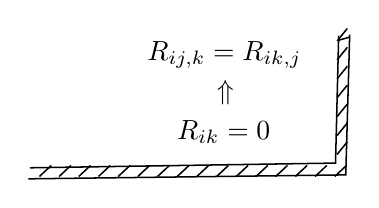
\begin{tikzpicture}[line width=.55pt]
\node at (.39,1.47) {\(R_{ij,k}=R_{ik,j}\)};
\node at (.40,.99) {\(\Uparrow\)};
\node at (.38,.49) {\(R_{ik}=0\)};
\draw (-2.08,.04)--(1.80,.10)--(1.84,1.72);
\draw (-2.10,-.10)--(1.93,-.05)--(1.98,1.73);
\draw (1.84,1.66)--(1.98,1.70);
\foreach \x in {-1.96,-1.71,...,1.79}
  \draw (\x,-.07)--++(.15,.14);
\foreach \y in {.21,.45,...,1.65}
  \draw (1.82,\y)--++(.13,.16);
\end{tikzpicture}}\endgroup\par
Двойная стрелка идёт вверх. Снизу и справа заштрихованный угол.}
\end{GelfandAdjacentEvidence}



\Needspace{7\baselineskip}
\begin{GelfandAdjacentEvidence}{GELFAND-P000678}{1}
\SourcePage{GELFAND-P000678}{unlabelled}
\underline{Сем. Гельфанда.}

\underline{И. Н. Бернштейн.}

\underline{Костант.}
\[
\begin{aligned}
\underline{\varphi(x)=\prod_{n=1}^{\infty}(1-x^n)
   =(1-x)(1-x^2)(1-x^3)\times\ldots}\\
=\sum_{n=-\infty}^{\infty}(-1)^n x^{(3n^2+n)/2}.
\end{aligned}
\]
\Unclear{GELFAND-P000678}{euler-product}{Нижний предел произведения густо наведён и читается как \(n=1\).}
\end{GelfandAdjacentEvidence}
\begin{GelfandAdjacentEvidence}{GELFAND-P000678}{2}

\Unclear{GELFAND-P000678}{euler-factor-mark}{Между третьим множителем и многоточием тёмный знак, похожий на \(\times\).}
\end{GelfandAdjacentEvidence}
\begin{GelfandAdjacentEvidence}{GELFAND-P000678}{3}

\SourceFigure{GELFAND-P000678}{euler-arrow}{%
\par\smallskip
\begingroup\color{black}\GelfandFitDiagram{\begin{tikzpicture}[line width=.5pt]
\node[inner sep=0pt] at (1.36,.78) {\(=\sum\)};
\draw (-.05,.51)--(1.7,.51)--(1.7,.66);
\draw[->] (1.04,.10)--(1.30,.63);
\node[inner sep=0pt] at (1.00,-.15) {\uwave{Эйлер}.};
\end{tikzpicture}}\endgroup\par
Стрелка от имени указывает на равенство с суммой.}
\end{GelfandAdjacentEvidence}
\begin{GelfandAdjacentEvidence}{GELFAND-P000678}{4}


\underline{Якоби:}
\[
\varphi(x)^3=\sum_{n=0}^{\infty}(-1)^n(2n+1)x^{n(n+1)/2}
\]
(из \(\Theta\)-функции).
\Unclear{GELFAND-P000678}{jacobi-theta-case}{Овал с поперечной чертой передан прописной \(\Theta\).}
\end{GelfandAdjacentEvidence}
\begin{GelfandAdjacentEvidence}{GELFAND-P000678}{5}


С тех пор найдены другие (Дайсон и др.)

\uwave{Макдональд нашёл групп. основу.}

Легко пров., что
\[
\varphi(x)^{-1}=\sum p(n)x^n,
\]
\(p(n)\) --- число разб. числа \(n\) в сумму неотриц. слагаемых

\[
x\varphi(x)^{24}=\sum\tau(n)x^n,
\]
\(\tau(n)\) --- ф-я Рамануджана

это её определение

У \(\tau(n)\) есть комбинат. определение

\Incomplete{GELFAND-P000678}{dedekind-cancel}{Перечёркнутая запись над строкой «через».}
\end{GelfandAdjacentEvidence}
\begin{GelfandAdjacentEvidence}{GELFAND-P000678}{6}

(через \(\Theta\)-ф-ю Дедекинда)
\Unclear{GELFAND-P000678}{dedekind-theta-case}{Знак перед «ф-ю» передан как \(\Theta\), как в строке о формуле Якоби.}
\end{GelfandAdjacentEvidence}
\begin{GelfandAdjacentEvidence}{GELFAND-P000678}{7}


можно написать
\[
\varphi(x)^k,\quad \text{где }k\text{ --- размерность группы Ли (полупростой)}
\]
\SourceFigure{GELFAND-P000678}{step-table}{%
\par\smallskip
\begingroup\color{black}\GelfandFitDiagram{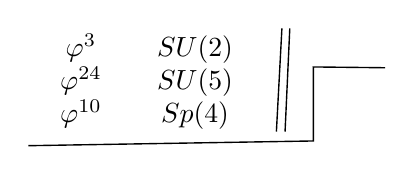
\begin{tikzpicture}[line width=.5pt]
\node[anchor=west,inner sep=0pt] at (.22,.80)
  {\(\begin{array}{c@{\qquad}c}
     \varphi^3&SU(2)\\
     \varphi^{24}&SU(5)\\
     \varphi^{10}&Sp(4)
   \end{array}\)};
\draw (3.15,.18)--(3.22,1.49) (3.26,.18)--(3.32,1.49);
\draw (0,0)--(3.62,.06)--(3.62,1.00)--(4.53,.99);
\end{tikzpicture}}\endgroup\par
Справа от трёх строк двойная черта. Под ними ступенчатая линия поднимается к следующему абзацу.}
\end{GelfandAdjacentEvidence}
\begin{GelfandAdjacentEvidence}{GELFAND-P000678}{8}


\dashuline{Макдональд}: явно выпис. ф-лу.

Пусть есть комп. полупростая группа
\Incomplete{GELFAND-P000678}{group-cancellations}{Две зачёркнутые записи между словом «группа» и обозначением.}
\end{GelfandAdjacentEvidence}
\begin{GelfandAdjacentEvidence}{GELFAND-P000678}{9}

\(G\)

\(g\) --- её алгебра Ли, на \(g\) есть форма Киллинга \(B\)

\(\Delta\) --- оператор Лапласа на
\Incomplete{GELFAND-P000678}{laplace-cancellations}{Две зачёркнутые записи после «на».}
\end{GelfandAdjacentEvidence}
\begin{GelfandAdjacentEvidence}{GELFAND-P000678}{10}

\(G\)

\(X_1,\ldots,X_k\) --- ортонорм. базис в \(g\).

В обёрт. алгебре
\SourceFigure{GELFAND-P000678}{enveloping-insertion}{%
\par\smallskip
\begingroup\color{black}\GelfandFitDiagram{\begin{tikzpicture}[line width=.5pt]
\node[anchor=west,inner sep=0pt] (word) at (0,.73) {алгебре};
\node[draw,ellipse,inner sep=1.7pt] (note) at (1.12,0) {\(U(g)\)};
\draw (note.north west) to[out=52,in=-120] (word.south east);
\draw (note.north east) to[out=118,in=-60] (word.south east);
\end{tikzpicture}}\endgroup\par
Под словом «алгебре» обведено \(U(g)\).}
\end{GelfandAdjacentEvidence}
\begin{GelfandAdjacentEvidence}{GELFAND-P000678}{11}

рассм. элемент
\Incomplete{GELFAND-P000678}{enveloping-cancel}{Зачёркнутая формула перед элементом.}
\end{GelfandAdjacentEvidence}

\(\Delta=\sum X_i^2\). он 2-стор. инвариантен.


\Needspace{7\baselineskip}
\begin{GelfandAdjacentEvidence}{GELFAND-P000679}{1}
\SourcePage{GELFAND-P000679}{unlabelled}
\[
\varphi(x)^k=\sum_{\text{непр. предст. }V}
c_V\cdot\dim V\cdot x^{\left.\Delta\right|_V}
\]
\Incomplete{GELFAND-P000679}{top-exponent-cancellation}{Зачёркнутая запись в показателе перед \(\Delta|_V\).}
\end{GelfandAdjacentEvidence}
\begin{GelfandAdjacentEvidence}{GELFAND-P000679}{2}


(\(\left.\Delta\right|_V\) кратен единичному;
соб. значение \(\left.\Delta\right|_V\).
\SourceFigure{GELFAND-P000679}{irreducible-insertion}{%
\par\smallskip
\begingroup\color{black}\GelfandFitDiagram{\begin{tikzpicture}[line width=.5pt]
\node[inner sep=2pt] (note) {на непр. предст.};
\draw (note.north west)--(note.north east) to[out=0,in=0] (note.south east)
      --([xshift=6pt]note.south west) to[out=180,in=65] ([yshift=-9pt]note.south west);
\draw ([yshift=-2pt]note.north west)--([yshift=-9pt]note.south west);
\end{tikzpicture}}\endgroup\par
Вставка над строкой указывает на место после \(\Delta|_V\).}
\end{GelfandAdjacentEvidence}
\begin{GelfandAdjacentEvidence}{GELFAND-P000679}{3}


\sout{Отсюда} Асимптотика зав. от размерности.
\Unclear{GELFAND-P000679}{top-word-cancellation}{Зачёркнутое слово предположительно читается «Отсюда».}
\end{GelfandAdjacentEvidence}
\begin{GelfandAdjacentEvidence}{GELFAND-P000679}{4}


Группы быв. разные и ф-лы тоже.
\[
c_V=\chi_V(a),\qquad
\text{где }\underset{\text{некий элемент}}{a\in G}
\]

\sout{Для серии.} Для \(SU(n)\) есть единств. регул. элемент.
(класс сопр. элементов;) т.е. такой, что соб. знач. различны и
\Incomplete{GELFAND-P000679}{su-n-power-cancellation}{Зачёркнутый знак перед \(n\)-й степенью.}
\end{GelfandAdjacentEvidence}
\begin{GelfandAdjacentEvidence}{GELFAND-P000679}{5}

\(n\)-я степень скалярна.

\Incomplete{GELFAND-P000679}{matrix-left-cancellation}{Зачёркнутый знак слева от скобки матрицы.}
\end{GelfandAdjacentEvidence}
\begin{GelfandAdjacentEvidence}{GELFAND-P000679}{6}

\[
\begin{pmatrix}
 \xi&&&&0\\
 &\xi^2&&&\\
 &&\xi^3&&\\
 &&&\ddots&\\
 0&&&&\xi^n
\end{pmatrix}c,\qquad c\quad \text{\uwave{подобр., чтобы} }\det=1.
\]

Рассм. \(\zeta\)-функцию опер. Лапласа.

\uwave{В. Кац} --- док-во \underline{через}
\(\underline{\infty}\)-мерные алгебры Ли.

Рассм. \(-\Delta+\dfrac{\dim g}{24}\) и положим
\[
\zeta(s)\underset{\mathrm{def}}{=}
\left.\left(-\Delta+\frac{\dim g}{24}\right)^{-s}\right|_a
\]
\Incomplete{GELFAND-P000679}{zeta-definition-cancellation}{Зачёркнутая запись после знака определения.}
\end{GelfandAdjacentEvidence}
\begin{GelfandAdjacentEvidence}{GELFAND-P000679}{7}

(опер. свёртки с ф-ей,
\Unclear{GELFAND-P000679}{kernel-comment-cancellations}{Два перечёркнутых фрагмента. Во втором предположительно видно «ядро».}
\end{GelfandAdjacentEvidence}
\begin{GelfandAdjacentEvidence}{GELFAND-P000679}{8}

пост. на кл. сопр. элем.,
берётся знач. её в т. \(a\))

\(K(x,y)\) --- ядро. На самом деле \(K(xy^{-1})\)

Про \sout{\(\zeta(s)\)} что-то можно сказать
\Unclear{GELFAND-P000679}{pro-zeta-cancellation}{Зачёркнутый фрагмент предположительно читается \(\zeta(s)\).}
\end{GelfandAdjacentEvidence}
\begin{GelfandAdjacentEvidence}{GELFAND-P000679}{9}


\underline{Теорема.}
\SourceFigure{GELFAND-P000679}{theorem-bracket}{%
\par\smallskip
\begingroup\color{black}\GelfandFitDiagram{\begin{tikzpicture}[line width=.5pt]
\node[inner sep=2pt] (formula) {\(\zeta(s)=\zeta\left(\dfrac{\dim g}{2}-s\right)\)};
\draw ([yshift=3pt]formula.south west)--(formula.south west)--
      (formula.south east)--([yshift=3pt]formula.south east);
\end{tikzpicture}}\endgroup\par
Под формулой черта с поднятыми концами.}
\end{GelfandAdjacentEvidence}
\begin{GelfandAdjacentEvidence}{GELFAND-P000679}{10}

\Unclear{GELFAND-P000679}{dimension-letter}{Во всех трёх формулах знак после \(\dim\) передан как \(g\).}
\end{GelfandAdjacentEvidence}
\begin{GelfandAdjacentEvidence}{GELFAND-P000679}{11}


Теорема эквив.
\Incomplete{GELFAND-P000679}{theorem-word-cancellation}{Зачёркнутое слово после «эквив.».}
\end{GelfandAdjacentEvidence}
\begin{GelfandAdjacentEvidence}{GELFAND-P000679}{12}

тожд. для \(\varphi(x)^k\).

Есть ещё \(\varphi^{39},\ \varphi^{45}\qquad\text{Van Esh}\)
\Unclear{GELFAND-P000679}{van-esh-name}{Имя написано латиницей «Van Esh».}
\end{GelfandAdjacentEvidence}
\begin{GelfandAdjacentEvidence}{GELFAND-P000679}{13}


см. \underline{Garland, Lepowsky}, Inv. math., 34 (1976), 37--76

\noindent\rule{13mm}{.45pt}\enspace\(\cdot\)\enspace\rule{14mm}{.45pt}

\Incomplete{GELFAND-P000679}{olshanetsky-preceding-cancellation}{Подчёркнутое слово перед фамилией зачёркнуто.}
\end{GelfandAdjacentEvidence}
\begin{GelfandAdjacentEvidence}{GELFAND-P000679}{14}

\underline{Ольшанецкий.}

\(\Delta^0\) --- рад. часть опер. Лапласа.
\SourceFigure{GELFAND-P000679}{symmetric-space-insertion}{%
\par\smallskip
\begingroup\color{black}\GelfandFitDiagram{\begin{tikzpicture}[line width=.5pt]
\node[inner sep=2pt] (note) {на симметр. пр-ве};
\draw ([yshift=2pt]note.south west) to[out=-90,in=180]
      ([xshift=-4pt]note.south) to[out=0,in=130] ([yshift=-7pt]note.south)
      to[out=50,in=180] ([xshift=4pt]note.south) to[out=0,in=-110]
      ([yshift=4pt]note.south east);
\end{tikzpicture}}\endgroup\par
Вставка стоит над строкой после «Лапласа».}
\end{GelfandAdjacentEvidence}
\begin{GelfandAdjacentEvidence}{GELFAND-P000679}{15}

Он запис. в виде
\[
\longrightarrow\frac12\frac{\partial^2}{\partial t_k^2}
 +U(t_1,\ldots,t_n)
\]
\[
U=g\sum_{k>\ell}\frac1{\sin^2(t_k-t_\ell)}
\]
И есть полн. сист. наблюдаемых в квант. смысле.

\noindent\rule{14mm}{.45pt}\enspace\(\cdot\)\enspace\rule{15mm}{.45pt}

\underline{\underline{И. Бернштейн.}}\qquad
\underline{\underline{о раб. В. Г. Каца.}}

\underline{Конструкция алг. Ли по матрице Картана.}

\(\underset{n\times n}{(a_{ij})}\) --- матрица с целыми элем., у к-рой
\[
a_{ij}<0\quad\text{при }i\ne j
\qquad\Vert\qquad
\begin{aligned}
a_{ii}&=2,\\
a_{ij}\ne0&\Rightarrow a_{ji}\ne0
\end{aligned}
\]
(нули встр. симметрично)
\Unclear{GELFAND-P000679}{cartan-strict-inequality}{Знак между \(a_{ij}\) и нулём написан без нижней черты.}
\end{GelfandAdjacentEvidence}
\begin{GelfandAdjacentEvidence}{GELFAND-P000679}{16}

\Unclear{GELFAND-P000679}{cartan-zero-comment}{Окончание последнего слова сближено со скобкой. Читается предположительно «симметрично».}
\end{GelfandAdjacentEvidence}



\Needspace{7\baselineskip}
\begin{GelfandAdjacentEvidence}{GELFAND-P000680}{1}
\SourcePage{GELFAND-P000680}{unlabelled}
\SourceFigure{GELFAND-P000680}{left-rule}{%
\begingroup\color{black}\GelfandFitDiagram{\begin{tikzpicture}[line width=.5pt]
\draw (0,0)--(0,.85)--(.12,.85);
\end{tikzpicture}}\endgroup\enspace Вертикальная черта вдоль левого поля.}
\end{GelfandAdjacentEvidence}
\begin{GelfandAdjacentEvidence}{GELFAND-P000680}{2}


По такой матр. строится алг. Ли.

Рассм. \(h_i,e_i,f_i\) --- своб. образующие (\(n\) штук) и напишем соотношения

\SourceFigure{GELFAND-P000680}{relation-outline}{%
\begingroup\color{black}\GelfandFitDiagram{\begin{tikzpicture}[line width=.5pt]
\node[inner sep=3pt] (relations) {\(\begin{aligned}
\relax[h_i,e_j]&=-a_{ij}e_j,\\
[h_i,f_j]&=+a_{ij}f_j.\\
[h_i,h_j]&=0,\\
[e_i,f_i]&=h_i\cdot\delta_{ij}
\end{aligned}\)};
\draw (relations.south west)--(relations.south east)--(relations.north east);
\end{tikzpicture}}\endgroup\par
Система обведена снизу и справа.}
\end{GelfandAdjacentEvidence}
\begin{GelfandAdjacentEvidence}{GELFAND-P000680}{3}

\Unclear{GELFAND-P000680}{generator-signs}{Перед \(a_{ij}\) в первой строке стоит минус, во второй --- плюс.}
\end{GelfandAdjacentEvidence}
\begin{GelfandAdjacentEvidence}{GELFAND-P000680}{4}

\Unclear{GELFAND-P000680}{ef-generator-indices}{В последней строке у \(e\) и \(f\) читается один и тот же индекс \(i\).}
\end{GelfandAdjacentEvidence}
\begin{GelfandAdjacentEvidence}{GELFAND-P000680}{5}


(факторизуем своб. алг. по этим соотн.)
и факторизуем эту алг. по \(\max\) норм. подалгебре
[Вставлено слева над формулой: и ещё соотнош.]
\Unclear{GELFAND-P000680}{relations-insertion}{Последнее слово сокращено до «соотнош.».}
\end{GelfandAdjacentEvidence}
\begin{GelfandAdjacentEvidence}{GELFAND-P000680}{6}

\[
\underbrace{[e_i[e_i[e_i\ldots[e_i}_{-a_{ij}+1},e_j]]\mathord{..}]=0
\]
\Unclear{GELFAND-P000680}{nested-bracket-count}{Подчёркивающая скобка кончается перед запятой. После \(e_j\) видны две закрывающие скобки, две точки и ещё одна закрывающая скобка.}
\end{GelfandAdjacentEvidence}
\begin{GelfandAdjacentEvidence}{GELFAND-P000680}{7}


Для нек-рых матр. возникают классич. группы.
\(SU(2)\qquad e_+,h_+,f_+\qquad\text{матр. }1\times1\Vert(2)\)
\Unclear{GELFAND-P000680}{su-two-basis-indices}{У всех трёх букв написан нижний плюс.}
\end{GelfandAdjacentEvidence}
\begin{GelfandAdjacentEvidence}{GELFAND-P000680}{8}

\[
[h,e]=2e,\qquad[h,f]=-2f,\qquad[e,f]=h,
\]
\(SU(3)\) получ. для матр. \(\begin{pmatrix}2&-1\\-1&2\end{pmatrix}\).

О \underline{корнях}: \underline{Серр} «Группы и алгебры Ли» ---
читать только этот параграф.

Если \(a_{ij}=a_{ji}\), то верно утверждение:

Группа конечномерна \(\Leftrightarrow\) матр. полож. определена.
\[
\begin{pmatrix}
2&-1&-1\\
-1&2&-1\\
-1&-1&2
\end{pmatrix}
\quad\text{--- бесконечномерное расширение }SU(3).
\]
\underline{В. Г. Кац.}\ : фактор этой алг. по 1-мерн. центру есть
\[
SU(3)\otimes\mathbb C[x,x^{-1}].
\]
\[
[x^kg,x^\ell g']=x^{k+\ell}[g,g'].
\]
все нестрог. опред. так получаются.
\Unclear{GELFAND-P000680}{loop-wording}{Два слова сокращены: «нестрог. опред.».}
\end{GelfandAdjacentEvidence}


\uwave{С Новым Годом!}


\Needspace{7\baselineskip}
\begin{GelfandAdjacentEvidence}{GELFAND-P000681}{1}
\SourcePage{GELFAND-P000681}{unlabelled}

\underline{14/II-77.}\qquad\underline{Сем. Гельфанда.}

\underline{Ю. И. Манин.}

\dashuline{Калоджеро}: бумерон:
\SourceFigure{GELFAND-P000681}{upper-wave-sketch}{%
\begingroup\color{black}\GelfandFitDiagram{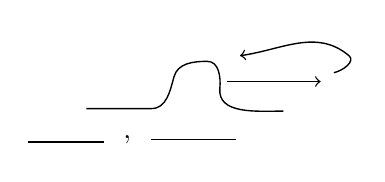
\begin{tikzpicture}[x=8mm,y=8mm,line width=.5pt]
\draw (0,.15) to[out=0,in=180] (1.03,.15)
  to[out=0,in=-105] (1.39,.65) to[out=75,in=180] (1.92,.9)
  to[out=0,in=85] (2.12,.47) to[out=-95,in=180] (3.13,.11);
\draw[->] (3.93,.72) to[out=12,in=-40] (4.17,.99)
  to[out=140,in=8] (2.44,.99);
\draw[->] (2.24,.58)--(3.72,.58);
\draw (-.92,-.38)--(.28,-.38) (1.03,-.34)--(2.38,-.34);
\node at (.65,-.35) {,};
\end{tikzpicture}}\endgroup\par
У верхней стрелки загиб справа. Между загибом и остриём нижней стрелки виден промежуток.}
\end{GelfandAdjacentEvidence}
\begin{GelfandAdjacentEvidence}{GELFAND-P000681}{2}

\Unclear{GELFAND-P000681}{boomeron-heading}{Под «Калоджеро» прерывистая черта. Следующее слово читается «бумерон».}
\end{GelfandAdjacentEvidence}
\begin{GelfandAdjacentEvidence}{GELFAND-P000681}{3}


Ур-е Лаксовского типа
\[
\overset{\text{\textcircled{\scriptsize 4}}}{L}_t=
[\overset{\text{\textcircled{\scriptsize 4}}}{L},
 \overset{\text{\textcircled{\scriptsize 2}}}{P}]
\]
\Unclear{GELFAND-P000681}{circled-orders}{Над обоими \(L\) стоит обведённая цифра 4, над \(P\) --- обведённая 2.}
\end{GelfandAdjacentEvidence}
\begin{GelfandAdjacentEvidence}{GELFAND-P000681}{4}

\[
L=\partial^4+v\partial^2+w\partial+z,\qquad
\partial=\partial/\partial x.
\]
\[
P=\partial^2+A\partial+u
\]
\(u\) выраж. через \(v,w,z\).
\[
\left\{\begin{aligned}
v_t&=v_{xx}-Av_x-2w_x\\
w_t&=2v_{xxx}+2vv_x-w_{xx}-Aw_x-2z_x\\
z_t&=\tfrac12v_{xxxx}+\tfrac12vv_{xx}+\tfrac12v_xw-z_{xx}-Az_x
\end{aligned}\right.
\]
\Unclear{GELFAND-P000681}{evolution-coefficients}{В первой строке перед \(v_{xx}\) множитель отсутствует. Во второй перед \(vv_x\) написано 2.}
\end{GelfandAdjacentEvidence}
\begin{GelfandAdjacentEvidence}{GELFAND-P000681}{5}


1-солитонное решение
\[
\mu_1=2\frac{\operatorname{ch}2\xi-\cos 2\xi+2\sin\sigma t}
               {\operatorname{ch}2\xi+\cos 2\xi-2\cos\sigma t}
\]
\[
\mu_2=2\frac{\operatorname{sh}2\xi-\sin 2\xi}
               {\operatorname{ch}2\xi+\cos 2\xi-2\cos\sigma t}
\]
\Unclear{GELFAND-P000681}{mu-two-raised-mark}{Справа вверху от множителя \(2\), перед \(\operatorname{sh}\), утолщённый знак. Возможно, это зачёркнутая цифра.}
\end{GelfandAdjacentEvidence}
\begin{GelfandAdjacentEvidence}{GELFAND-P000681}{6}

\[
\xi=x+ct\qquad
\begin{aligned}
c&\in\mathbb R\\
\sigma&\in\mathbb R\\
\sigma&\leftrightarrow A\quad\text{(выражается).}
\end{aligned}
\]
\[
\left\{\begin{aligned}
v&=-4\mu_{2x}\\
\sigma w&=4\mu_2\mu_{2x}+6\mu_{2xx}+4\mu_{1x}\\
z&=.\;.\;.\;.\qquad\text{(несущественно)}
\end{aligned}\right.
\]
\Unclear{GELFAND-P000681}{sigma-w}{В левой части второй строки написано \(\sigma w\).}
\end{GelfandAdjacentEvidence}
\begin{GelfandAdjacentEvidence}{GELFAND-P000681}{7}


\SourceFigure{GELFAND-P000681}{lower-mu-one-sketch}{%
\begingroup\color{black}\GelfandFitDiagram{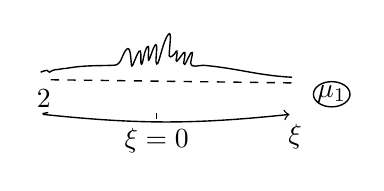
\begin{tikzpicture}[x=8mm,y=8mm,line width=.5pt]
\draw[dashed] (.23,.65)--(4.08,.6);
\node[below] at (.12,.65) {\(2\)};
\draw (.07,.77) to[out=15,in=180] (.17,.8)
  to[out=0,in=200] (.21,.77) to[out=25,in=185] (.3,.81)
  to[out=0,in=180] (.47,.83) to[out=10,in=182] (1.23,.88)
  to[out=0,in=-130] (1.43,1.13) to[out=50,in=95] (1.51,.89)
  to[out=-85,in=-125] (1.63,1.10) to[out=55,in=90] (1.66,.92)
  to[out=-75,in=-125] (1.76,1.17) to[out=55,in=95] (1.78,.98)
  to[out=-90,in=-120] (1.88,1.19) to[out=55,in=90] (1.90,.94)
  to[out=-80,in=-125] (2.09,1.36) to[out=55,in=90] (2.11,1.03)
  to[out=-75,in=-110] (2.22,1.10) to[out=55,in=80] (2.22,.96)
  to[out=-90,in=-135] (2.34,1.08) to[out=45,in=85] (2.34,.91)
  to[out=-80,in=-130] (2.46,1.08) to[out=45,in=85] (2.45,.91)
  to[out=-80,in=180] (2.65,.88) to[out=-5,in=177] (4.06,.69);
\draw[->] (.11,.1) to[out=-6,in=186] (4.02,.1);
\draw (.11,.1) to[out=130,in=210] (.19,.13);
\draw (1.91,.03)--(1.91,.13);
\node[below] at (1.91,.03) {\(\xi=0\)};
\node[below] at (4.11,.10) {\(\xi\)};
\draw (4.69,.42) ellipse (.29 and .20);
\node at (4.69,.42) {\(\mu_1\)};
\end{tikzpicture}}\endgroup\par
У левого конца оси виден крючок и мелкие неразборчивые штрихи.}
\end{GelfandAdjacentEvidence}
\begin{GelfandAdjacentEvidence}{GELFAND-P000681}{8}


[Справа от графика:] каждые \(\dfrac{2\pi}{\sigma}\) периодически
\Incomplete{GELFAND-P000681}{periodic-comment-cancellation}{В конце строки зачёркнут знак или короткая запись.}
\end{GelfandAdjacentEvidence}

плюётся
(гейзерон, плюон, \(.\;.\;.\;.\))
взрывная неустойчивость.

\underline{Алг. способ.}

а) строим вспом. стац. ур-е
\([L_1,P_1]=0\)\qquad затем ввод. \(t\).

б)
\[
\left\{\begin{aligned}
L_1\psi&=\lambda\psi\\
P_1\psi&=\mu\psi
\end{aligned}\right.
\qquad
(\lambda,\mu)\in X\quad\text{--- афф. алг. кривая}
\]
было исслед.: \underline{\(\dim(\text{пр-ва }\psi)=1\)}.

У Кричевера явно не ук., но вытек. из ограничений.

\underline{Дринфельд} --- не указ. явно реш., но указ. трудности.


\Needspace{7\baselineskip}
\begin{GelfandAdjacentEvidence}{GELFAND-P000682}{1}
\SourcePage{GELFAND-P000682}{unlabelled}
\SourceFigure{GELFAND-P000682}{top-fibre-diagram}{%
\begingroup\color{black}\GelfandFitDiagram{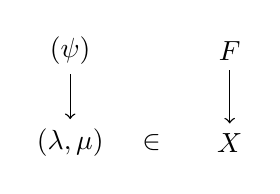
\begin{tikzpicture}[x=9mm,y=9mm,line width=.5pt]
\node (psi) at (0,1.3) {\((\psi)\)};
\node (pair) at (0,0) {\((\lambda,\mu)\)};
\node at (1.15,0) {\(\in\)};
\node (fibre) at (2.25,1.3) {\(F\)};
\node (base) at (2.25,0) {\(X\)};
\draw[->] (psi)--(pair);
\draw[->] (fibre)--(base);
\end{tikzpicture}}\endgroup\par
Две стрелки направлены вниз. Между нижними записями стоит знак, переданный как \(\in\).}
\end{GelfandAdjacentEvidence}
\begin{GelfandAdjacentEvidence}{GELFAND-P000682}{2}

\Unclear{GELFAND-P000682}{top-map-symbol}{Знак в скобках читается как \(\psi\). В середине виден дополнительный тонкий штрих.}
\end{GelfandAdjacentEvidence}
\begin{GelfandAdjacentEvidence}{GELFAND-P000682}{3}


Рассл. продолж. на пополнение.
\Unclear{GELFAND-P000682}{top-opening-abbreviations}{Среднее слово сокращено и предположительно читается «продолж.».}
\end{GelfandAdjacentEvidence}
\begin{GelfandAdjacentEvidence}{GELFAND-P000682}{4}

Получаем рассл. на кривой
\[
t\longrightarrow\text{путь по Якобиану.}
\]
\[
\underset{\text{Модули системы;}}{\underline{\underline{r>1}}}
\quad\Rightarrow\quad\text{путь в модулях расслоений.}
\]
Гиперэлл. кривая \(\longrightarrow\) пересеч. 2-х квадрик в \(\mathbb C^5\).
\Unclear{GELFAND-P000682}{hyperelliptic-ambient}{После «в» написано \(\mathbb C^5\).}
\end{GelfandAdjacentEvidence}
\begin{GelfandAdjacentEvidence}{GELFAND-P000682}{5}

Аналит. пути?

Солитон --- реш. нестац. ур-я, к-рое получ. если в стац. ур-и берётся кривая с 1-й двойной точкой с раздел. касательными.

\underline{Обозначения}. \(k\) --- поле хар-ки 0.
\[
\underset{\text{в аналит. вар.,}}{(k=\mathbb R\ \text{или}\ \mathbb C)}
\]
\(\mathcal B\) --- \(k\)-алг.
\[
\left(\begin{aligned}
\mathcal B&=\underset{\text{матрицы}}{M_\ell}(\mathcal B_0),\\
\mathcal B_0&=\text{поле рац. }k\text{-анал. }
          \overset{\text{мером.}}{\text{ф-й}}\ \text{от }
          \begin{matrix}x\\x,t\\x,t,z\end{matrix}
\end{aligned}\right)
\]
\Unclear{GELFAND-P000682}{meromorphic-insertion}{Над промежутком перед «ф-й» вписано «мером.» с фигурной отводкой.}
\end{GelfandAdjacentEvidence}
\begin{GelfandAdjacentEvidence}{GELFAND-P000682}{6}


\[
\underset{\text{дифференцирования}}{\partial,\partial_1,\partial_2:\mathcal B\longrightarrow\mathcal B},
\qquad [\partial,\partial_i]=[\partial_i,\partial_j]=0
\]
(в ан. вар. \(\partial=\partial/\partial x\), \(\partial_1=\partial/\partial t\),
\(\partial_2=\partial/\partial z\)).

\(\mathcal B[\partial]\)

\((L,P)\) --- пара оп. уд. одному из 3-х ур-й
\[
\left\{\begin{aligned}
\relax[L,P]&=0 &&\text{стац. Лакс}\\
\partial_1 L&=[L,P] &&\text{нестац. Лакс}\\
\partial_1 L+\partial_2 P&=[L,P] &&\text{Зах.-Шабат}
\end{aligned}\right.
\]

\textcircled{1}\enspace \underline{Бимодуль Крич.-Дринфельда \(\mathcal M\)}.
\Unclear{GELFAND-P000682}{circled-section}{Обведённая 1 слева от заголовка.}
\end{GelfandAdjacentEvidence}
\begin{GelfandAdjacentEvidence}{GELFAND-P000682}{7}


\underline{Структуры}.

а) \(\mathcal M\) --- \(k\)-лин. пр-во, левый \(\mathcal B\)-модуль, правый \(\mathcal O\)-модуль, где

\(\mathcal O\) --- кольцо ф-й на афф. кривой над \(k\); непривод. над \(\bar k\).

б) отмеч. элемент \(\mathbf 1\in\mathcal M\)

в) возраст. фильтрация
\[
\mathcal M_{-1}\subset\mathcal M_0\subset\mathcal M_1\subset\mathcal M_2\subset\ldots,
\qquad\bigcup_{i=0}^\infty\mathcal M_i=\mathcal M
\]
г) \(\nabla:\mathcal M\longrightarrow\mathcal M\qquad k\)-лин. оператор.

\underline{Аксиомы}.

д) действия \(\overset{\mathcal B\text{ и }\mathcal O}{\text{эффективны}}\) и коммутируют
\Unclear{GELFAND-P000682}{action-insertion}{«\(\mathcal B\) и \(\mathcal O\)» вписано над промежутком после «действия» с фигурной отводкой.}
\end{GelfandAdjacentEvidence}
\begin{GelfandAdjacentEvidence}{GELFAND-P000682}{8}


е) \(\mathcal M_{-1}=0,\qquad \mathcal B\mathcal M_i\subset\mathcal M_i\)

ж) \(\mathcal M_i/\mathcal M_{i-1}\) --- своб. \(\mathcal B\)-модуль ранга \(1;\qquad \mathcal M_0=\mathcal B\mathbf 1\).

з)
\[
\forall b\in\mathcal B,\ m\in\mathcal M:\quad
\nabla(bm)=(\partial b)m+b\nabla m,
\]
\[
\forall\varphi\in\mathcal O,\qquad
(\nabla m)\varphi=\nabla(m\varphi)
\]
\Unclear{GELFAND-P000682}{bottom-retraced-phi}{Буква в \((\nabla m)\varphi\) обведена. По двум соседним написаниям читается \(\varphi\).}
\end{GelfandAdjacentEvidence}



\Needspace{7\baselineskip}
\begin{GelfandAdjacentEvidence}{GELFAND-P000683}{1}
\SourcePage{GELFAND-P000683}{unlabelled}

(«набла» --- название старинного муз. инструмента типа лиры).

и)
\[
\begin{aligned}
&\forall i\geq-1,\qquad\nabla\mathcal M_i\subset\mathcal M_{i+1},\\
&\nabla:\mathcal M_i/\mathcal M_{i-1}
   \overset{\sim}{\longrightarrow}\mathcal M_{i+1}/\mathcal M_i
\end{aligned}
\]
\Unclear{GELFAND-P000683}{filtration-lower-bound}{В начале строки написано \(i\geq-1\).}
\end{GelfandAdjacentEvidence}
\begin{GelfandAdjacentEvidence}{GELFAND-P000683}{2}


\textcircled{2}\enspace Конструкция бимодуля по паре \(L,P\in\mathcal B[\partial]\)
с \([L,P]=0\) и \(\bar k[L,P]\) без делителей нуля.

Положим
\[
\mathcal M=\mathcal B[\partial];\qquad \mathcal O=k[L,P].
\]
--- кольцо мн-ов от \(L\) и \(P\).

действие \(\mathcal B\) --- умн. слева, действие \(\mathcal O\) --- умн. справа

\(\mathbf1=\) тождеств. оператор
\[
\mathcal M_i=\left\{\sum_{k\leq i}b_k\partial^k\mid b_k\in\mathcal B\right\}.
\qquad
\nabla m=\partial\circ m
\]
Аксиомы проверяются тривиально.

\underline{Теорема 1}. Если есть \((\mathcal B,\mathcal O)\)-бимодуль
\(\mathcal M\), то по нему строится вложение \(i:\mathcal O\longrightarrow\mathcal B[\partial]\),
такое что при обратной конструкции из \(i\) получается \(\mathcal M\).

\(\overline{\underline{\text{Конструкция}}}\).

а)
\SourceFigure{GELFAND-P000683}{endomorphism-diagram}{%
\begingroup\color{black}\GelfandFitDiagram{\begin{tikzpicture}[x=9mm,y=9mm,line width=.5pt]
\node (nabla) at (0,1.45) {\(\mathcal B[\nabla]\)};
\node (d) at (0,0) {\(\mathcal B[\partial]\)};
\node[anchor=west,inner sep=1pt,align=left] at (1.05,1.45)
  {--- эндоморфизмы\\
   \(\mathcal M\longrightarrow\mathcal M\).};
\node[anchor=west,inner sep=1pt] at (1.05,0)
  {\(\mathcal M\cong\mathcal B[\nabla]\mathbf1\)};
\draw[->] (nabla)--(d);
\draw (.28,.96) to[out=0,in=75] (.38,.83)
  to[out=-105,in=180] (.38,.62);
\end{tikzpicture}}\endgroup}
\end{GelfandAdjacentEvidence}
\begin{GelfandAdjacentEvidence}{GELFAND-P000683}{3}

\Unclear{GELFAND-P000683}{construction-vertical-arrow}{Справа от стрелки вниз отдельный вертикальный волнистый штрих.}
\end{GelfandAdjacentEvidence}
\begin{GelfandAdjacentEvidence}{GELFAND-P000683}{4}

Здесь не использовалось умн. на \(\mathcal O\).

б)
\SourceFigure{GELFAND-P000683}{embedding-diagram}{%
\begingroup\color{black}\GelfandFitDiagram{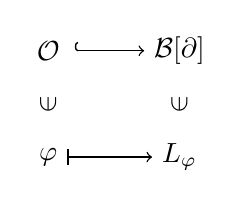
\begin{tikzpicture}[x=9mm,y=9mm,line width=.5pt]
\node (o) at (0,1.5) {\(\mathcal O\)};
\node (d) at (1.85,1.5) {\(\mathcal B[\partial]\)};
\node (phi) at (0,0) {\(\varphi\)};
\node (l) at (1.85,0) {\(L_\varphi\)};
\coordinate (hook) at ([xshift=3pt]o.east);
\draw[->] (hook)--(d);
\draw (hook) to[out=180,in=180] ([yshift=3pt]hook);
\draw[|->] (phi)--(l);
\node[rotate=90,inner sep=0pt] at (0,.75) {\(\in\)};
\node[rotate=90,inner sep=0pt] at (1.85,.75) {\(\in\)};
\end{tikzpicture}}\endgroup\par
тч. \(L_\varphi\mathbf1=\mathbf1\varphi\).
\par
(этим опр. \(L_\varphi\)).}
\end{GelfandAdjacentEvidence}
\begin{GelfandAdjacentEvidence}{GELFAND-P000683}{5}


\underline{Теорема 2}. Пусть дана \((\mathcal O,\mathcal B)\)-бимодуль
\(\mathcal M\) и диффер. \(\partial_1:\mathcal B\longrightarrow\mathcal B\)
(в анал. вар. \(\partial/\partial t\)), а также пусть есть
\(\nabla_1:\mathcal M\longrightarrow\mathcal M\)
\Unclear{GELFAND-P000683}{theorem-two-module-order}{В формулировке теоремы 2 сначала написано \(\mathcal O\), затем \(\mathcal B\).}
\end{GelfandAdjacentEvidence}
\begin{GelfandAdjacentEvidence}{GELFAND-P000683}{6}

\[
\left\{\begin{aligned}
\nabla_1(bm)&=\partial_1b+\nabla_1m\\
\nabla_1(m\varphi)&=(\nabla_1m)\varphi\\
[\nabla_1,\nabla]&=0
\end{aligned}\right.
\]
\Unclear{GELFAND-P000683}{theorem-two-first-relation}{В правой части видны только \(\partial_1b\) и \(\nabla_1m\), со знаком плюс между ними.}
\end{GelfandAdjacentEvidence}
\begin{GelfandAdjacentEvidence}{GELFAND-P000683}{7}

\[
[\mathcal M,\nabla_1]\longrightarrow\text{серия реш. нестац. ур-й Лакса}
\]
\[
\begin{gathered}
\nabla_1\mathbf1=P\mathbf1,\qquad P\in B[\partial].\\
\mathbf1\varphi=L_\varphi\mathbf1
\end{gathered}
\]
Тогда
\SourceFigure{GELFAND-P000683}{bottom-lax-outline}{%
\begingroup\color{black}\GelfandFitDiagram{\begin{tikzpicture}[line width=.5pt]
\node[inner sep=3pt] (eq)
 {\(\partial_1L_\varphi=\text{[зач.]}\pm[P,L_\varphi]\)};
\draw ([yshift=4pt]eq.south west)--(eq.south west)--(eq.south east)
      --([yshift=4pt]eq.south east);
\end{tikzpicture}}\endgroup}
\end{GelfandAdjacentEvidence}
\begin{GelfandAdjacentEvidence}{GELFAND-P000683}{8}

\Incomplete{GELFAND-P000683}{bottom-cancelled-symbol}{Между знаком равенства и \(\pm\) зачёркнут знак.}
\end{GelfandAdjacentEvidence}
\begin{GelfandAdjacentEvidence}{GELFAND-P000683}{9}

\SourceFigure{GELFAND-P000683}{fixed-p-callout}{%
\begingroup\color{black}\GelfandFitDiagram{\begin{tikzpicture}[line width=.5pt]
\draw (0,0)--(0,-.85) (.08,0)--(.08,-.85);
\node[anchor=north west,align=left,inner sep=0pt] at (.22,.06)
  {Здесь \(P\) фиксировано\\а \(L\) варьируется.};
\end{tikzpicture}}\endgroup}
\end{GelfandAdjacentEvidence}



\Needspace{7\baselineskip}
\begin{GelfandAdjacentEvidence}{GELFAND-P000684}{1}
\SourcePage{GELFAND-P000684}{unlabelled}

\underline{Теорема} 3. Дан модуль \(\mathcal M\) \uwave{без упоминаний об} \(\mathcal O\).
\Unclear{GELFAND-P000684}{without-o-wavy-underline}{Волнистая черта под словами «без упоминаний об» оканчивается перед \(\mathcal O\).}
\end{GelfandAdjacentEvidence}
\begin{GelfandAdjacentEvidence}{GELFAND-P000684}{2}


\(\nabla,\nabla_1,\nabla_2\) попарно коммутируют. Тогда получ. реш. ур-й Зах.-Шабата:
\[
\begin{gathered}
\nabla_1\mathbf1=P\mathbf1\\
\nabla_2\mathbf1=L\mathbf1\\
\partial_2P+\partial_1L=\pm[L,P].
\end{gathered}
\]
\Unclear{GELFAND-P000684}{zakharov-shabat-signs}{Между двумя производными стоит плюс, перед коммутатором --- \(\pm\).}
\end{GelfandAdjacentEvidence}
\begin{GelfandAdjacentEvidence}{GELFAND-P000684}{3}


Следующий раз \underline{Дюйстермаат}.
\Unclear{GELFAND-P000684}{duistermaat-name}{Фамилия подчёркнута и читается «Дюйстермаат».}
\end{GelfandAdjacentEvidence}
\begin{GelfandAdjacentEvidence}{GELFAND-P000684}{4}


\SourceFigure{GELFAND-P000684}{closing-separator}{%
\begingroup\color{black}\GelfandFitDiagram{\begin{tikzpicture}[line width=.5pt]
\draw (0,0) to[out=135,in=210] (.13,.035)--(1.46,.035);
\fill (1.83,.035) circle (.7pt);
\draw (2.32,.045)--(4.13,.10);
\end{tikzpicture}}\endgroup\par
У левого конца короткой линии небольшой загиб. Две линии разделены точкой.}
\end{GelfandAdjacentEvidence}



\Needspace{7\baselineskip}
\begin{GelfandAdjacentEvidence}{GELFAND-P000685}{1}
\SourcePage{GELFAND-P000685}{unlabelled}

\underline{21/II-77 г.}\qquad \underline{Сем. Гельфанда.}

\underline{Дейстермаат.}
\Unclear{GELFAND-P000685}{name-spelling}{Фамилия здесь написана «Дейстермаат».}
\end{GelfandAdjacentEvidence}
\begin{GelfandAdjacentEvidence}{GELFAND-P000685}{2}


\underline{Об индексе Морса.}

\(I(\gamma)\) --- функционал, \(\gamma\) --- крив. в \(\mathbb R^n\),
\sout{\(\gamma\in H^1\) (пр-во Соболева)}
\Unclear{GELFAND-P000685}{crossed-sobolev}{Зачёркнута запись \(\gamma\in H^1\) с пояснением в скобках.}
\end{GelfandAdjacentEvidence}
\begin{GelfandAdjacentEvidence}{GELFAND-P000685}{3}

\[
I(\gamma)=\int_0^T f(\gamma(t),\dot\gamma(t))\,dt
\]
Вариационная задача.
\[
\gamma\in\text{space of curves such thet }(\gamma(0),\gamma(T))\in R
\]
\Unclear{GELFAND-P000685}{original-english}{Строка написана по-английски. Слово после «such» предположительно читается «thet».}
\end{GelfandAdjacentEvidence}
\begin{GelfandAdjacentEvidence}{GELFAND-P000685}{4}


\(R\) --- подмн-зие в \(\mathbb R^n\times\mathbb R^n\).

Примеры; а) \(R=(0,0)\in\mathbb R^n\times\mathbb R^n\) --- закрепл. концы

б) \(R=\{(x,x)\}\quad\text{---}\quad\gamma(0)=\gamma(T)\) --- периодич. условие
\Unclear{GELFAND-P000685}{periodic-separator}{Между формулами утолщённый горизонтальный штрих, переданный как черта.}
\end{GelfandAdjacentEvidence}


Экстремаль --- критич. точка в \(H^1\).
\[
\begin{aligned}
\text{Если }&\frac{\partial^2 f}{\partial\dot\gamma^2}>0,
&\text{то }\operatorname{ind}\frac{\partial^2 I}{\partial\gamma^2}&<\infty\\
&\text{(полож. опр.)}
&\text{(число отриц. квадр. конечно)}&
\end{aligned}
\]


\Needspace{7\baselineskip}
\begin{GelfandAdjacentEvidence}{GELFAND-P000686}{1}
\SourcePage{GELFAND-P000686}{unlabelled}
\[
\operatorname{ind}\frac{\partial^2 I}{\partial\gamma^2}
=\text{индекс Морса гран. условия}=\operatorname{ind}_R(\gamma).
\]
Будет ф-ла для индекса Морса через индекс Арнольда кривой на лагр. мн-зии.

\underline{Теорема.}
\[
\text{Morse }\operatorname{index}_R(\gamma)
=\operatorname{ind}(\varphi)+i(I,\rho,\varphi(T))
  +\dim\pi(\rho\cap I)-2n.
\]
\Unclear{GELFAND-P000686}{index-theorem-tail}{В правой части читаются \(i(I,\rho,\varphi(T))\) и \(\dim\pi(\rho\cap I)-2n\).}
\end{GelfandAdjacentEvidence}
\begin{GelfandAdjacentEvidence}{GELFAND-P000686}{2}


\noindent Ур-е для стац. кривых (Эйлера--Лагранжа)
\(\underset{\text{пр. Лежандра}}{\longrightarrow}\)
ур-е Гамильтона
\[
(\gamma,\dot\gamma)\underset{\text{преобр. Лежандра}}{\mapsto}
\]

Гамильт. ур. опр. поток симпл. преобразований.

Рассм. ур-е в вар. вдоль экстремали. Получим 1-пар. сем-во лин. симплектич. преобразований.

\(\Phi(t)=\) производная гамильт. потока вдоль экстрем. кривой

это лин. преобр.:
\[
\underset{\substack{\text{фазовое}\\\text{пр-во}}}{\mathbb R_\sigma^{2n}}
\longrightarrow \mathbb R_\sigma^{2n}
\]
\Unclear{GELFAND-P000686}{flow-domain-subscript}{Нижний индекс первого \(\mathbb R^{2n}\) сильно обведён и читается предположительно как \(\sigma\).}
\end{GelfandAdjacentEvidence}
\begin{GelfandAdjacentEvidence}{GELFAND-P000686}{3}

\Unclear{GELFAND-P000686}{flow-codomain-subscript}{Нижний индекс второго \(\mathbb R^{2n}\) также сильно обведён и читается предположительно как \(\sigma\).}
\end{GelfandAdjacentEvidence}
\begin{GelfandAdjacentEvidence}{GELFAND-P000686}{4}

\[
\varphi(t)=\operatorname{graph}\varphi(t)\subset
\underline{\mathbb R_\sigma^{2n}\times\mathbb R_{-\sigma}^{2n}}
\qquad \text{(симпл. структ. --- разность)}
\]
\Unclear{GELFAND-P000686}{graph-letter}{Знак после «graph» выглядит строчным и передан как \(\varphi\).}
\end{GelfandAdjacentEvidence}
\begin{GelfandAdjacentEvidence}{GELFAND-P000686}{5}

\[
\Phi(t)^*\sigma=\sigma.\qquad t\ \text{фиксир.}
\]
\[
\Updownarrow
\]
\SourceFigure{GELFAND-P000686}{pullback-letter}{%
\begingroup\color{black}\GelfandFitDiagram{\begin{tikzpicture}[line width=.5pt]
\node[inner sep=3pt] (eq) {\(\sigma-\varphi(t)^*\sigma=0\)};
\draw ([yshift=4pt]eq.south west)--(eq.south west)--(eq.south east)
     --([yshift=4pt]eq.south east);
\end{tikzpicture}}\endgroup\par
Под чертой с поднятыми концами нет подписи. Буква перед \((t)\) передана как строчная \(\varphi\).}
\end{GelfandAdjacentEvidence}
\begin{GelfandAdjacentEvidence}{GELFAND-P000686}{6}


или
\[
\underline{\sigma\oplus(-\sigma)=0\text{ на }\varphi(t)}
\]
\Incomplete{GELFAND-P000686}{cancelled-before-lagrangian}{Запись перед скобкой густо зачёркнута.}
\end{GelfandAdjacentEvidence}
\begin{GelfandAdjacentEvidence}{GELFAND-P000686}{7}

\uwave{(лагранжево подпр-во)}

\SourceFigure{GELFAND-P000686}{lagrangian-planes-sketch}{%
\begingroup\color{black}\GelfandFitDiagram{\begin{tikzpicture}[line width=.5pt]
\draw (.19,1.42) .. controls (.17,.8) and (-.05,-.40) .. (-.04,-.62);
\draw (-.22,.07) .. controls (.60,-.04) and (1.65,-.06) .. (2.24,-.05);
\draw (-.77,-.62)--(2.37,1.16);
\draw (-.70,-.51) .. controls (-.89,-.57) and (-.86,-.71) .. (-.66,-.61);
\node at (0,1.65) {\(\beta\)};
\node at (2.20,-.49) {\(\alpha\)};
\node at (2.72,1.30) {\(\gamma\)};
\end{tikzpicture}}\endgroup\par
Три штриха с подписями \(\alpha,\beta,\gamma\) сходятся около одной точки.}
\end{GelfandAdjacentEvidence}
\begin{GelfandAdjacentEvidence}{GELFAND-P000686}{8}

\(\alpha,\beta,\gamma\) --- 3 лагр. плоск.
\[
\begin{aligned}
\alpha\cap\beta&=0\\
\gamma\cap\beta&=0
\end{aligned}
\]

Тогда можно считать
\[
\gamma=\operatorname{graph}\Gamma,\qquad
\Gamma\ \text{линейно}\ :\alpha\to\beta
\]
\Incomplete{GELFAND-P000686}{linear-overwritten-sign}{После «линейно» перед двоеточием переписан один знак.}
\end{GelfandAdjacentEvidence}
\begin{GelfandAdjacentEvidence}{GELFAND-P000686}{9}

\[
Q(u,v)=\sigma(\Gamma u,v),\qquad u,v\in\alpha
\]
Получили билин. форму на \(\alpha\)
\[
\sigma=0\text{ на }\Gamma\quad\Leftrightarrow\quad Q\text{ симметрична.}
\]
\Incomplete{GELFAND-P000686}{cancelled-before-q}{Запись перед \(Q=Q(\alpha,\beta,\gamma)\) густо зачёркнута.}
\end{GelfandAdjacentEvidence}
\begin{GelfandAdjacentEvidence}{GELFAND-P000686}{10}

\[
Q=Q(\alpha,\beta,\gamma)
\]
Если \(\underset{\text{(кривая лагр. плоск.)}}{\gamma=\gamma(t)}\), то в какой-то мом. \(\gamma\) может пересечься с \(\alpha\)
по 1-мерн. подпр..

В мом. пересеч. надо взять разность индексов \underline{(она не зав. от выб. \(\beta\))}.

\([\gamma:\alpha]\) --- индекс пересечения кривой \(\gamma(t)\) с гиперповерхн.
\[
\Sigma_\alpha=\{\gamma\mid\gamma\cap\alpha\ne0\}.
\]
\Unclear{GELFAND-P000686}{overwritten-hypersurface}{Конец слова переписан. Сокращение предположительно читается «гиперповерхн.».}
\end{GelfandAdjacentEvidence}



\Needspace{7\baselineskip}
\begin{GelfandAdjacentEvidence}{GELFAND-P000687}{1}
\SourcePage{GELFAND-P000687}{unlabelled}

\SourceFigure{GELFAND-P000687}{top-crossing-sketch}{%
\begingroup\color{black}\GelfandFitDiagram{\begin{tikzpicture}[x=9mm,y=9mm,line width=.5pt]
\node at (-.42,2.67) {\(\Sigma_\alpha\)};
\draw (-.23,2.43) to[out=-28,in=126] (.37,1.84) to[out=-53,in=116] (1.51,.16);
\draw (1.46,2.52) to[out=-115,in=3] (1.23,2.30)
  to[out=168,in=11] (.79,2.45) to[out=-170,in=24] (.28,2.27)
  to[out=-158,in=75] (-.21,1.51) to[out=-105,in=174] (.00,1.22)
  to[out=-3,in=-166] (.76,1.52) to[out=14,in=95] (1.22,1.27)
  to[out=-86,in=46] (1.04,.60) to[out=-133,in=36] (.22,-.06);
\draw (1.46,2.52) to[out=60,in=4] (1.44,2.57) to[out=188,in=94] (1.42,2.51);
\node at (.71,1.69) {\(+\)};
\node at (1.49,.69) {\(+\)};
\draw (.41,1.08)--(.48,.94) (.97,.43)--(1.08,.30);
\end{tikzpicture}}\endgroup\par
Извилистая линия трижды пересекает \(\Sigma_\alpha\). У двух пересечений по плюсу и короткому штриху. У верхнего конца кривой маленькая петля.}
\end{GelfandAdjacentEvidence}
\begin{GelfandAdjacentEvidence}{GELFAND-P000687}{2}

\(\Rightarrow\) это гомотопич. инвар. при фиксир. концах.

\(\Sigma_\alpha\) влож. двусторонне
\Incomplete{GELFAND-P000687}{top-cancelled}{После открывающей скобки зачёркнута запись.}
\end{GelfandAdjacentEvidence}
\begin{GelfandAdjacentEvidence}{GELFAND-P000687}{3}


Отсюда \(\pi_1(\text{лагр. плоскости})=\mathbb Z\)
\[
\begin{aligned}
\text{т.к. }(\text{лагр. пл.})
   &=\Sigma_\alpha\cup(\text{трансверс. плоск.})\\
   &\hphantom{=\Sigma_\alpha\cup{}}\quad\ \Vert\\
   &\hphantom{=\Sigma_\alpha\cup{}}(\text{квадр. формы})
      \quad\text{--- гомот. трив.}
\end{aligned}
\]
Нач. и кон. точки, не леж. в \(\Sigma_\alpha\), можно соединить в доп. и гомот. тип, ни от чего не зависит.
\Unclear{GELFAND-P000687}{endpoint-word}{Конец строки читается «в доп.».}
\end{GelfandAdjacentEvidence}
\begin{GelfandAdjacentEvidence}{GELFAND-P000687}{4}

\Unclear{GELFAND-P000687}{endpoint-reading}{Перед «в доп.» читается «можно соединить».}
\end{GelfandAdjacentEvidence}
\begin{GelfandAdjacentEvidence}{GELFAND-P000687}{5}


Для незамкнутой кривой:
\[
\operatorname{ind}(\gamma)=[\gamma:\alpha]
 +\operatorname{ind}Q\{\gamma(T),\alpha,\gamma(0)\}
\]
(чтобы не зависело от \(\alpha\)).

\SourceFigure{GELFAND-P000687}{n-one-arrow}{%
\begingroup\color{black}\GelfandFitDiagram{\begin{tikzpicture}[line width=.5pt]
\node[inner sep=1pt] (n) {\(n=1\)};
\draw[->] (n.south west)--(n.south east);
\end{tikzpicture}}\endgroup}
\end{GelfandAdjacentEvidence}
\begin{GelfandAdjacentEvidence}{GELFAND-P000687}{6}

лагр. плоск. --- окружность

\SourceFigure{GELFAND-P000687}{circle-sketch}{%
\begingroup\color{black}\GelfandFitDiagram{\begin{tikzpicture}[x=9mm,y=9mm,line width=.5pt]
\draw (0,-.61)--(0,1.06) (-1.01,0)--(1.17,.06) (-.61,.56)--(.81,-.47)
      (-.25,-.93)--(.30,.91) (-.67,-.63)--(.85,.75) (-1.00,-.42)--(1.13,.52);
\draw[->] (-.07,.76)--(-.07,.43);
\draw (3.94,.56) to[out=-129,in=153] (3.58,-.15)
      to[out=-30,in=208] (4.27,-.22) to[out=27,in=-108] (4.70,.45);
\draw[dashed] (3.94,.56) to[out=37,in=123] (4.70,.45);
\fill (3.94,.56) circle (1pt) (4.70,.45) circle (1pt);
\end{tikzpicture}}\endgroup\par
Слева пучок прямых со стрелкой вниз. На окружности верхняя дуга пунктирная, её концы отмечены густыми штрихами.}
\end{GelfandAdjacentEvidence}
\begin{GelfandAdjacentEvidence}{GELFAND-P000687}{7}

[Справа от рисунков:] досоединить незамкн. по час. стрелке, от нач. точки к конечной.
\Unclear{GELFAND-P000687}{circle-verb}{Начало слова читается предположительно «до», затем «соединить».}
\end{GelfandAdjacentEvidence}
\begin{GelfandAdjacentEvidence}{GELFAND-P000687}{8}


\(\operatorname{ind}(\gamma)\) --- получ. число оборотов.

\(R\) --- мн-зие гр. условий

\[
\begin{aligned}
R^\perp&=\text{норм. расслоение}\\
 &=\left\{\underset{\mathbb R^{2n}}{(x,\xi)},
        \underset{\mathbb R^{2n}}{(y,-\eta)}
      \ \middle|\ (\xi,\eta)\perp T_{(x,y)}R\right\}.
\end{aligned}
\]
\[
\rho=T_{(\ ,\ )}(R^\perp)
\]
\Incomplete{GELFAND-P000687}{tangent-cancelled}{Первоначальный индекс при \(T\) зачёркнут. Ниже написаны пустые скобки с запятой.}
\end{GelfandAdjacentEvidence}
\begin{GelfandAdjacentEvidence}{GELFAND-P000687}{9}

--- слой норм. рассл. над т. экстремали
\Unclear{GELFAND-P000687}{normal-point-word}{Последнее слово предположительно «экстремали». Часть штрихов может быть зачёркиванием.}
\end{GelfandAdjacentEvidence}
\begin{GelfandAdjacentEvidence}{GELFAND-P000687}{10}


это лагранжева плоскость

\[
i(I,\rho,\varphi(T))=
(\operatorname{ind}+\operatorname{null})Q(I,\rho,\varphi(T))
\]
\SourceFigure{GELFAND-P000687}{negative-zero-callout}{%
\begingroup\color{black}\GelfandFitDiagram{\begin{tikzpicture}[line width=.5pt]
\node[anchor=west,inner sep=1pt] at (.18,.48) {отриц. \(+0\)-е квадраты.};
\draw[->] (.34,.39)--(.07,.13);
\end{tikzpicture}}\endgroup}
\end{GelfandAdjacentEvidence}
\begin{GelfandAdjacentEvidence}{GELFAND-P000687}{11}


\(I\) --- график [вставлено сверху: тожд.] отобр.
\Incomplete{GELFAND-P000687}{identity-cancelled}{Слово между «график» и «отобр.» зачёркнуто.}
\end{GelfandAdjacentEvidence}
\begin{GelfandAdjacentEvidence}{GELFAND-P000687}{12}

\Unclear{GELFAND-P000687}{identity-insertion}{Вставка над зачёркиванием предположительно «тожд.».}
\end{GelfandAdjacentEvidence}
\begin{GelfandAdjacentEvidence}{GELFAND-P000687}{13}


\(\pi\) --- проекция на базу.

\underline{\underline{Формула следа Сельберга.}}\qquad \underline{в простейшем случае}:

\(G\) --- полупр. связная вещ. гр. Ли, \(K\) --- \(\max\) комп. подгр., \(K\backslash G\)
\SourceFigure{GELFAND-P000687}{noncompact-callout}{%
\begingroup\color{black}\GelfandFitDiagram{\begin{tikzpicture}[line width=.5pt]
\node (top) at (0,.74) {\(K\backslash G\)};
\node (label) [align=center,inner sep=1pt] at (0,0) {симметр. пр.\\некомп. типа};
\draw (label.north)--(top.south);
\end{tikzpicture}}\endgroup}
\end{GelfandAdjacentEvidence}


\(\Gamma\) --- дискретная подгр. \(G\), действ. на \(M=K\backslash G\) справа.

\(M/\Gamma=X\) --- компактное мн-зие.

Будут рассм. все опер. \(C^\infty(M)\to C^\infty(M)\),
коммутир. с действ. \(G\).
\[
f\longmapsto\varphi*f,\qquad
(\varphi*f)(x)=\int_G\varphi(xy^{-1})f(y)\,dy
\]
\[
\varphi\in\mathcal E'(K\backslash G)
\]


\Needspace{7\baselineskip}
\begin{GelfandAdjacentEvidence}{GELFAND-P000688}{1}
\SourcePage{GELFAND-P000688}{unlabelled}

\(f\) инвар. \(\Rightarrow\) можно счит.
\(\varphi\in\mathcal E'(K\backslash G/K)\)
(двустор. инв.) --- сферич. ф-и.

Оператор на \(X\) имеет ядро Шварца.

Для \(\varphi\) сосред. в \(e\in G\) получ. дифф. оператор.

Формула --- для спектра дифф. опер. на \(M\), спущ. на \(X\).

Положим
\[
K_\varphi(x,y)=\sum_{\gamma\in\Gamma}\varphi(x\gamma y^{-1})
\]

Легко видеть из инвар., что \(K_\varphi\in\mathcal E'(X\times X)\).

Рассм. теперь опер. с гладким \(\varphi\) (финитным).

\(\Gamma\) --- дискр. \(\Rightarrow\) [переписано] сумма для фикс. \(x,y\) конечна.
\Incomplete{GELFAND-P000688}{sum-cancelled}{Перед словом «сумма» густо переписан один знак.}
\end{GelfandAdjacentEvidence}
\begin{GelfandAdjacentEvidence}{GELFAND-P000688}{2}

\[
\varphi\in C_c^\infty(K\backslash G/K)
\quad\Rightarrow\quad K_\varphi\in C^\infty(X\times X).
\]

Имеем:
\[
K_\varphi\circ K_\psi=K_{\varphi*\psi}
\]
\[
\varphi*\psi=\psi*\varphi\qquad\text{на сферич. ф-ях}
\]

\(\Rightarrow\) получ. коммут. алг. опер. \(K_\varphi\) с инвол.
Все они комп. \(\Rightarrow\)

\(\Rightarrow\ \exists\) ортон. базис общ. соб. вект. \(e_j\in L^2(X)\)
\[
K_\varphi(e_j)=\lambda_j(\varphi)e_j,\qquad
\forall\varphi\in C_c^\infty(K\backslash G/K)
\]

Имеем:
\[
\begin{aligned}
\sum_j\lambda_j(\varphi)
&=\operatorname{Sp}K_\varphi
 =\int_XK_\varphi(x,x)\,dx\\
&=\sum_{\gamma\in\Gamma}\int_X
 \varphi\bigl(x_{?}\gamma_{?}x^{-1}\bigr)\,dx
\end{aligned}
\]
\Unclear{GELFAND-P000688}{trace-lower-marks}{Под первым \(x\) и под \(\gamma\) видны два похожих мелких знака. Их чтение не установлено.}
\end{GelfandAdjacentEvidence}
\begin{GelfandAdjacentEvidence}{GELFAND-P000688}{3}

\[
\bigl(C_c^\infty(K\backslash G/K),*\bigr)
\overset{\sim}{\longrightarrow} C_c^\infty(A)^W,\qquad
W\ \text{--- гр. Вейля}
\]
\Unclear{GELFAND-P000688}{spherical-delimiter}{После последнего \(K\) перед запятой густо переписана скобка.}
\end{GelfandAdjacentEvidence}
\begin{GelfandAdjacentEvidence}{GELFAND-P000688}{4}


\SourceFigure{GELFAND-P000688}{iwasawa-callouts}{%
\begingroup\color{black}\GelfandFitDiagram{\begin{tikzpicture}[x=9mm,y=9mm,line width=.5pt]
\node at (-1.0,.3) {\(G=\)};
\node (k) at (0,.3) {\(K\)};
\node (a) at (.83,.3) {\(A\)};
\node (n) at (1.67,.3) {\(N\)};
\node[anchor=north east,inner sep=1pt] (ck) at (.14,-.30) {комп.};
\node[anchor=north west,inner sep=1pt] (un) at (1.52,-.30) {унипот.};
\node[align=center,inner sep=1pt] (diag) at (1.15,-1.28) {диаг. с полож.\\диаг. эл.};
\draw (k.south)--(0,-.30) (n.south)--(1.67,-.30) (a.south)--(.83,-.85);
\end{tikzpicture}}\endgroup\par
--- разл. Ивасавы.}
\end{GelfandAdjacentEvidence}
\begin{GelfandAdjacentEvidence}{GELFAND-P000688}{5}

\Unclear{GELFAND-P000688}{iwasawa-name}{В рукописи фамилия читается «Ивасавы».}
\end{GelfandAdjacentEvidence}
\begin{GelfandAdjacentEvidence}{GELFAND-P000688}{6}


\[
f(a)=e^{\langle\rho,a\rangle}\int_N\varphi(an)\,dn.
\]
(орисферическое отобр. \(\varphi\mapsto f\)).

Имеем:
\[
\lambda_j(\varphi*\psi)=\lambda_j(\varphi)\cdot\lambda_j(\psi).
\]

Отсюда
\[
\lambda_j(\varphi)=\langle f,e^{i\mu_j}\rangle
 =\widetilde f_{?}(\mu_j),\qquad\mu_j\in A_{\mathbb C}^*.
\]
\Unclear{GELFAND-P000688}{fourier-lower-mark}{Под \(\widetilde f\) есть отдельный неразобранный знак.}
\end{GelfandAdjacentEvidence}
\begin{GelfandAdjacentEvidence}{GELFAND-P000688}{7}

[Справа на поле:] \underline{\(A\) --- вект. пр-во}
\Unclear{GELFAND-P000688}{vector-space-margin}{Подпись про \(A\) вынесена вправо и подчёркнута.}
\end{GelfandAdjacentEvidence}
\begin{GelfandAdjacentEvidence}{GELFAND-P000688}{8}


Здесь \(\rho=\dfrac12\sum\text{пол. корней}\)

\Incomplete{GELFAND-P000688}{bottom-cancelled}{Короткое слово над «Имеем» зачёркнуто.}
\end{GelfandAdjacentEvidence}

Имеем:
\[
\sum_j\lambda_j(\varphi)=\sum_{\gamma\in\Gamma}\langle T_\gamma,f\rangle,
\]
(каждое слаг. переписали)

\(T_\gamma\) --- лок. конечн. сем. распред.


\Needspace{7\baselineskip}
\begin{GelfandAdjacentEvidence}{GELFAND-P000689}{1}
\SourcePage{GELFAND-P000689}{unlabelled}

Все встр. скобочки таинств. образом исчезают
\Unclear{GELFAND-P000689}{top-noun}{Слово после «встр.» предположительно читается «скобочки».}
\end{GelfandAdjacentEvidence}
\begin{GelfandAdjacentEvidence}{GELFAND-P000689}{2}

\[
\sum_j\widetilde f(\mu_j)
=\sum_{\gamma\in\Gamma}\langle T_\gamma,f\rangle,\qquad
f\in C_c^\infty(A)^W
\]
где \(T_\gamma\in\mathcal D'(A)^W\)

\SourceFigure{GELFAND-P000689}{spectral-parameter-outline}{%
\begingroup\color{black}\GelfandFitDiagram{\begin{tikzpicture}[line width=.5pt]
\node[inner sep=3pt] (eq) {\(\mu_j\in A_{\mathbb C}^*\)};
\draw ([yshift=4pt]eq.south west)--(eq.south west)--(eq.south east)
     --([yshift=4pt]eq.south east);
\end{tikzpicture}}\endgroup}
\end{GelfandAdjacentEvidence}
\begin{GelfandAdjacentEvidence}{GELFAND-P000689}{3}

--- счётн. набор точек, наз. спектром [зачёркнуто] \underline{\(\operatorname{Spec}\)}.
\Incomplete{GELFAND-P000689}{cancelled-before-spec}{Перед «Spec» густо зачёркнуты короткие знаки.}
\end{GelfandAdjacentEvidence}
\begin{GelfandAdjacentEvidence}{GELFAND-P000689}{4}


Далее: информация о \(\mu_j\) по \(T_\gamma\), зад. явными интегралами.
\[
T_\gamma(f)=\int_X\varphi(x\gamma x^{-1})\,dx,\qquad
f(a)=(\ \ )\int\varphi(an)\,dn
\]
\Unclear{GELFAND-P000689}{empty-abel-factor}{Перед интегралом в формуле для \(f(a)\) стоят пустые скобки.}
\end{GelfandAdjacentEvidence}
\begin{GelfandAdjacentEvidence}{GELFAND-P000689}{5}

\[
T_e(f)=\varphi(e)\cdot\operatorname{vol}(X)
\]
\Incomplete{GELFAND-P000689}{cancelled-before-harish}{Короткая запись перед фамилией зачёркнута.}
\end{GelfandAdjacentEvidence}
\begin{GelfandAdjacentEvidence}{GELFAND-P000689}{6}

Хариш-Чандра
\[
T_e=\operatorname{vol}(X)\cdot\widetilde\beta,\qquad
\beta\text{ --- мера Планшереля.}
\]

\(\ell(\gamma)\) --- длина замкн. геодезич., отв. классу фунд. гр.

\underline{Теорема.}
\SourceFigure{GELFAND-P000689}{length-theorem-outline}{%
\begingroup\color{black}\GelfandFitDiagram{\begin{tikzpicture}[line width=.5pt]
\node[inner sep=3pt] (eq)
  {\(\ell(\gamma)=\operatorname{dist}(\operatorname{supp}T_\gamma,0).\)};
\draw ([yshift=4pt]eq.south west)--(eq.south west)--(eq.south east)
     --([yshift=4pt]eq.south east);
\end{tikzpicture}}\endgroup}
\end{GelfandAdjacentEvidence}
\begin{GelfandAdjacentEvidence}{GELFAND-P000689}{7}


Итак,
\[
\sum_j\widetilde f(\mu_j)
=\langle\widetilde f,\beta\rangle\operatorname{vol}(X)
 +\sum_{\gamma\ne e}\langle T_\gamma,f\rangle.
\]

\SourceFigure{GELFAND-P000689}{closing-rules}{%
\begingroup\color{black}\GelfandFitDiagram{\begin{tikzpicture}[line width=.5pt]
\draw (.05,0)--(1.04,0) (1.90,0)--(3.24,0);
\fill (1.47,-.045) circle (.6pt);
\end{tikzpicture}}\endgroup}
\end{GelfandAdjacentEvidence}
\begin{GelfandAdjacentEvidence}{GELFAND-P000689}{8}


\[
\#\{j:|\mu_j|\le R\}
=\operatorname{vol}(X)\int_{\operatorname{ball}(R)}\beta
 +O(R^{n-r-1})
\]
\Unclear{GELFAND-P000689}{remainder-exponent}{Средний знак в показателе степени предположительно читается \(r\). Также возможна \(\tau\).}
\end{GelfandAdjacentEvidence}



\Needspace{7\baselineskip}
\begin{GelfandAdjacentEvidence}{GELFAND-P000690}{1}
\SourcePage{GELFAND-P000690}{unlabelled}

\underline{28/II-77 г.}\qquad\underline{Сем. Гельфанда.}

\underline{Манин} (продолжение).

\(k=\mathbb R\) или \(\mathbb C\),

\(\mathcal B_0\) --- алг. ростков \(k\)-мером. ф-й от \(x\) или \(x,t\)
или \(x,t,y\)
\[
\mathcal B=M_\ell(\mathcal B_0),\qquad
\partial_x,\partial_y,\partial_t:\mathcal B\to\mathcal B
\]
\Unclear{GELFAND-P000690}{matrix-order}{Под \(M\) в записи матричной алгебры читается \(\ell\).}
\end{GelfandAdjacentEvidence}
\begin{GelfandAdjacentEvidence}{GELFAND-P000690}{2}

\[
\mathcal B[\partial_x]
\]
Цель: отыск. пар. \(L,P\in\mathcal B[\partial_x]\), уд. одному из ур-й
\[
\begin{array}{ccccc}
[L,P]=0&\text{или}&L_t=[P,L]&\text{или}&L_t+P_y=[P,L]\\
\text{(стац. Лакс)}&&\text{(нестац. Лакс)}&&\text{(Зах.-Шабат)}
\end{array}
\]
\Unclear{GELFAND-P000690}{zakharov-shabat-order}{Справа в третьем уравнении коммутатор написан в порядке \([P,L]\).}
\end{GelfandAdjacentEvidence}
\begin{GelfandAdjacentEvidence}{GELFAND-P000690}{3}

\(\mathcal O\) --- кольцо ф-й на аффинной \(k\)-кривой. Пусть построено

\(k\)-пр-во \(M\), \((\mathcal B,\mathcal O)\)-бимодуль,
\[
0\subset M_0\subset M_1\subset\cdots
\quad\text{--- фильтр. }\mathcal B\text{-подмодулей}
\]
\[
\mathbf1\in M,\qquad \nabla:M\to M
\]
\Incomplete{GELFAND-P000690}{cancelled-connection-formula}{Под \(\nabla:M\to M\) зачёркнута формула. Различимы скобки и \(bm\).}
\end{GelfandAdjacentEvidence}
\begin{GelfandAdjacentEvidence}{GELFAND-P000690}{4}

\[
\nabla(bm)=(\partial_x b)\cdot m+b\cdot(\nabla m)
\]
Дополнит. аксиомы [зачёркнуто] см. выше.
\Incomplete{GELFAND-P000690}{cancelled-axioms-word}{Короткое слово перед «см.» перечёркнуто.}
\end{GelfandAdjacentEvidence}
\begin{GelfandAdjacentEvidence}{GELFAND-P000690}{5}


\underline{Пример} (основной)
\[
\mathcal O=k[L,P],\quad M=\mathcal B[\partial_x],\quad
\mathbf1=\operatorname{id},\quad\nabla=\partial\,[?]
\]
\Unclear{GELFAND-P000690}{example-derivative-index}{Справа от \(\partial\) видна петля, ниже несколько штрихов. Чтение нижнего знака как \(x\) не установлено.}
\end{GelfandAdjacentEvidence}
\begin{GelfandAdjacentEvidence}{GELFAND-P000690}{6}

\(L,P\) --- реш. стац. зад.

\sout{Определение.}
\Unclear{GELFAND-P000690}{cancelled-definition-heading}{Зачёркнутый заголовок предположительно читается «Определение».}
\end{GelfandAdjacentEvidence}
\begin{GelfandAdjacentEvidence}{GELFAND-P000690}{7}

\underline{Лемма}. \(M\) --- \(\mathcal B[\partial_x]\)-своб. модуль ранга \(1\)
с образ. \(\mathbf1\)

(\(\partial_x\) действ. через \(\nabla\))

\(\mathrm I\). \uwave{стац. Лакс}:
\[
\mathcal O\ni\varphi\mapsto L_\varphi\in\mathcal B[\partial_x],
\quad\mathbf1\varphi=L_\varphi\mathbf1
\quad\Rightarrow\quad[L_\varphi,L_\psi]=0
\]
\(\underline{\mathrm{II}}\). \uwave{нестац. Лакс}:
\[
\nabla_t:M\to M,\qquad [\nabla_x,\nabla_t]=0,
\]
\SourceFigure{GELFAND-P000690}{case-two-double-rule}{%
\begingroup\color{black}\GelfandFitDiagram{\begin{tikzpicture}[line width=.5pt]
\node[inner sep=3pt] (eq) {\(\begin{gathered}
\nabla_t\mathbf1=P\mathbf1\\
\text{[зачёркнуто]}\quad\mathbf1\varphi=L_\varphi\mathbf1
\end{gathered}\)};
\draw (eq.south east)--([xshift=5pt]eq.north east);
\draw ([xshift=3pt]eq.south east)--([xshift=8pt]eq.north east);
\end{tikzpicture}}\endgroup}
\end{GelfandAdjacentEvidence}
\begin{GelfandAdjacentEvidence}{GELFAND-P000690}{8}

\Incomplete{GELFAND-P000690}{cancelled-nonstationary-formula}{Короткая формула слева от \(\mathbf1\varphi=L_\varphi\mathbf1\) перечёркнута.}
\end{GelfandAdjacentEvidence}

\[
\Rightarrow L_t=[P,L]
\]


\Needspace{7\baselineskip}
\begin{GelfandAdjacentEvidence}{GELFAND-P000691}{1}
\SourcePage{GELFAND-P000691}{unlabelled}

\(\underline{\mathrm{III}}\). \(\nabla_y:M\to M\)
\[
\nabla_t,\nabla_y,\nabla_x
\quad\Rightarrow\quad\nabla_t\mathbf1=P\mathbf1,\qquad\nabla_y\mathbf1=L\mathbf1
\]

\underline{Явная конструкция класса бимодулей ранга \(r\geq1\)} (ранг)
\Unclear{GELFAND-P000691}{heading-rank}{После подчёркнутого \(r\geq1\) стоит «(ранг)».}
\end{GelfandAdjacentEvidence}
\begin{GelfandAdjacentEvidence}{GELFAND-P000691}{2}


\(\underline{r=1}\Rightarrow N\)-солит. реш. КдФ и высших КдФ.

Фиксируется \(N\geq1\) (колич. солитонов).
\[
\begin{gathered}
\alpha_1,\ldots,\alpha_N\in k,\qquad\alpha_i\ne\alpha_j\\
\beta_1,\ldots,\beta_N
\end{gathered}
\]
\(\alpha_i=\overline{\beta_i}\) при \(k=\) [зачёркнуто] \(\mathbb R\).
(смысл --- кривая веществ.)
\Incomplete{GELFAND-P000691}{cancelled-field-symbol}{Между \(k=\) и \(\mathbb R\) зачёркнут знак.}
\end{GelfandAdjacentEvidence}
\begin{GelfandAdjacentEvidence}{GELFAND-P000691}{3}

\Unclear{GELFAND-P000691}{reality-parenthesis}{Первое слово в скобках предположительно читается «смысл».}
\end{GelfandAdjacentEvidence}
\begin{GelfandAdjacentEvidence}{GELFAND-P000691}{4}

\[
\mathcal O=\{f\in k[\lambda]\mid f(\alpha_i)=f(\beta_i),\quad
\forall i=1,\ldots,N\}.
\]
Модуль --- сеч. рассл., поднятие тривиально.

\SourceFigure{GELFAND-P000691}{curve-sketches}{%
\begingroup\color{black}\GelfandFitDiagram{\begin{tikzpicture}[line width=.5pt]
\draw (.28,1.13) to[out=12,in=177] (1.36,1.15)
     to[out=-4,in=94] (2.83,.91) to[out=-80,in=10] (2.24,.59)
     to[out=186,in=6] (.60,.62) to[out=183,in=26] (.03,.38)
     to[out=206,in=-151] (.18,.34) to[out=22,in=220] (.64,.60);
\draw (.05,-.29) to[out=49,in=171] (.30,-.13)
     to[out=-9,in=87] (.49,-.24) to[out=-92,in=13] (.08,-.35)
     to[out=180,in=-145] (.05,-.29);
\draw (.47,-.26) to[out=36,in=186] (.75,-.08)
     to[out=6,in=68] (.96,-.19) to[out=-112,in=5] (.57,-.30)
     to[out=171,in=-128] (.47,-.26);
\draw (.96,-.19) to[out=-4,in=188] (1.49,-.17)
     to[out=0,in=48] (1.49,-.41) to[out=-130,in=-25] (1.15,-.46)
     to[out=150,in=-80] (.96,-.19);
\end{tikzpicture}}\endgroup\par
Две схемы без подписей. Верхняя вытянутая линия разомкнута слева, нижняя образует три петли.}
\end{GelfandAdjacentEvidence}
\begin{GelfandAdjacentEvidence}{GELFAND-P000691}{5}


Положим
\[
N=\mathcal B[\lambda]^r\quad\text{и}\quad N\supset M
\]
Все структуры на \(M\) индуц. структурами \(N\). Введ. на \(N\)
\[
\mathcal B\times N\to N,\quad\text{[зачёркнуто]}\quad N\times k[\lambda]\to N
\]
\Incomplete{GELFAND-P000691}{cancelled-action-word}{Между двумя действиями зачёркнуто короткое слово.}
\end{GelfandAdjacentEvidence}
\begin{GelfandAdjacentEvidence}{GELFAND-P000691}{6}

\[
b\begin{pmatrix}b_1(\lambda)\\\vdots\\b_r(\lambda)\end{pmatrix}
=\begin{pmatrix}b_1(\lambda)b^t\\\vdots\\b_r(\lambda)b^t\end{pmatrix}
\]
\Unclear{GELFAND-P000691}{action-transpose}{В обоих видимых компонентах правого столбца написано \(b^t\).}
\end{GelfandAdjacentEvidence}
\begin{GelfandAdjacentEvidence}{GELFAND-P000691}{7}

\[
\operatorname{GL}(\mathcal B[\lambda],r)\times N\to N
\]
\[
M=\{m(\lambda)\in N\mid m(\alpha_i)=g_i m(\beta_i),
\quad\forall i=1,\ldots,N\}
\]
(нетрив. усл. скл. в отлич. от ф-й)

\SourceFigure{GELFAND-P000691}{gl-coefficient}{%
\begingroup\color{black}\GelfandFitDiagram{\begin{tikzpicture}[line width=.5pt]
\node[inner sep=1pt] at (.10,.4) {\(g_i\in\operatorname{GL}(\mathbb C\,\mathcal B,r)\)};
\node[anchor=west,inner sep=0pt] at (.25,-.20) {комплексные};
\draw (.31,.19)--(.31,-.07);
\end{tikzpicture}}\endgroup\par
Между \(\mathbb C\) и \(\mathcal B\) явного знака операции не видно.}
\end{GelfandAdjacentEvidence}
\begin{GelfandAdjacentEvidence}{GELFAND-P000691}{8}

--- параметры (матрицы склейки, из них возник. нетрив. варианты).

\Incomplete{GELFAND-P000691}{cancelled-gluing-region}{Короткая запись перед условием сопряжения зачёркнута.}
\end{GelfandAdjacentEvidence}
\begin{GelfandAdjacentEvidence}{GELFAND-P000691}{9}

\[
\overline{g_i}=g_i^{-1}\quad\text{при }k=\mathbb R
\]

\uwave{Фильтрация на \(N\)}:
\[
\underset{0\leq k\leq r-1}{N_{ar+k}}
=\left\{
\begin{pmatrix}b_1\\\vdots\\b_r\end{pmatrix}\in\mathcal B[\lambda]^r
\ \middle|\
\begin{aligned}
b_1,\ldots,b_k&\text{ --- многоч. по }\lambda\text{ степ. }\leq a,\\
b_{k+1},\ldots,b_r&\text{ --- '' --- }\leq a-1
\end{aligned}\right\}
\]
\Unclear{GELFAND-P000691}{filtration-column}{Столбец в фигурной скобке начинается с \(b_1\) и заканчивается \(b_r\).}
\end{GelfandAdjacentEvidence}
\begin{GelfandAdjacentEvidence}{GELFAND-P000691}{10}

\Unclear{GELFAND-P000691}{filtration-ditto}{Во второй строке вместо повторённых слов две черты и два коротких наклонных штриха.}
\end{GelfandAdjacentEvidence}

\[
\mathcal B N_i\subset N_i,
\]
\(M\) начнётся не с того места (есть сист. лин. ур-й).
\[
M_{(i)}=M\cap N_i\quad\text{--- ещё не то}
\]
\underline{Лемма.} Рассм. матрицу (блочную)
\[
(\alpha_i^j\operatorname{Id}_r-\beta_i^j g_i)_{
\substack{i=1,\ldots,N\\j=0,\ldots,N-1}}
\]
Пусть
\[
\det(\alpha_i^j\operatorname{Id}_r-\beta_i^j g_i)\ne0.
\]


\Needspace{7\baselineskip}
\begin{GelfandAdjacentEvidence}{GELFAND-P000692}{1}
\SourcePage{GELFAND-P000692}{unlabelled}

Тогда \(M_{(rN)}=\{0\}\), \(\forall i>rN\) есть кан. вложение
\[
M_{(i)}/M_{(i-1)}\overset{\sim}{\longrightarrow}N_i/N_{i-1}
\]
является изоморфизмом.

\underline{Опред.}: \(M_i=M_{(i-rN)}\).
\Unclear{GELFAND-P000692}{filtration-shift}{В скобках индекса написано \(i-rN\).}
\end{GelfandAdjacentEvidence}
\begin{GelfandAdjacentEvidence}{GELFAND-P000692}{2}


Явный вид \(\mathbf1\) нах. из сист. лин. ур-й. Имеем:
\[
\mathbf{1}=\sum_{j=0}^{N-1}m_j\lambda^j+
\begin{pmatrix}\lambda^N\\0\\\cdot\\0\end{pmatrix}
\qquad\text{(по опред. \(M_1\)).}
\]
\Incomplete{GELFAND-P000692}{generator-cancel}{Под знаком равенства зачёркнута короткая запись.}
\end{GelfandAdjacentEvidence}
\begin{GelfandAdjacentEvidence}{GELFAND-P000692}{3}

\Unclear{GELFAND-P000692}{vector-entries}{Между двумя нулями в столбце видна одна точка.}
\end{GelfandAdjacentEvidence}
\begin{GelfandAdjacentEvidence}{GELFAND-P000692}{4}

Коэфф. при \(\lambda^N=1\) [зачёркнуто] --- усл. нормировки.
\Incomplete{GELFAND-P000692}{normalization-cancel}{После единицы зачёркнут знак.}
\end{GelfandAdjacentEvidence}
\begin{GelfandAdjacentEvidence}{GELFAND-P000692}{5}


\(m_j\) удовл. сист. лин. ур-й
\[
\begin{gathered}
\sum_{j=0}^{N-1}(\alpha_i^j E_r-\beta_i^j g_i)m_i+
(\alpha_i^N-\beta_i^N g_i)\begin{pmatrix}1\\0\\\vdots\\0\end{pmatrix}=0,\\
i=1,\ldots,N.
\end{gathered}
\]
\Unclear{GELFAND-P000692}{coefficient-index}{После первой скобки написано \(m_i\).}
\end{GelfandAdjacentEvidence}
\begin{GelfandAdjacentEvidence}{GELFAND-P000692}{6}

Отсюда однозначно нах. \(m_i\).

Вариант: \(\nabla_x\overset{?}{=}\partial_x\).
Усл. склейки нарушаются.

Добавим эндоморфизм модуля \(M\).
\[
\nabla_x=\partial_x+\underbrace{d_x(\lambda)}_{\text{матрица}},
\]
где
\[
d_x(\lambda)\in M_r(\mathcal B[\lambda])
=\operatorname{End}_{\mathcal B}(N=\mathcal B[\lambda]^r).
\]
\Incomplete{GELFAND-P000692}{endomorphism-cancel}{Перед \(M_r\) зачёркнут знак.}
\end{GelfandAdjacentEvidence}
\begin{GelfandAdjacentEvidence}{GELFAND-P000692}{7}


\underline{Лемма}. \(\nabla_x M\subset M\), \underline{если \(g_i\) уд. системе дифф. ур-й}
\[
\partial_xg_i=g_i d_x(\beta_i)-d_x(\alpha_i)g_i,\qquad i=1,\ldots,N.
\]
\underline{\(d_x\) --- матрица связности}. \underline{(вместо \(g_i\) включ. в геом. структуру)}.

\(d_x\) --- произвольный\qquad \(g_i\) --- находим.

Простейшие решения для \(g_i\):

Пусть \(d_x(\lambda)\in M_r(M_\ell(k))[\lambda]\). Тогда
(при фикс. \(\lambda=\mathrm{const}\))
\[
g_i(x)=\exp(-x d_x(\alpha_i))g_i(0)\exp(x d_x(\beta_i)).
\]

\underline{Доп. парам.}: матрицы \(d_x(\lambda)\) с пост. коэфф.

\(r=1\Rightarrow\) обычн. \(\exp\).

Аналогично \(\rightarrow\) пишутся ур-я для \(\nabla_t\).
\[
\begin{aligned}
\nabla_t&=\partial_t+d_t(\lambda)\\
\nabla_y&=\partial_y+d_y(\lambda).
\end{aligned}
\]

Коммутирование ?
\[
\underline{\partial_xd_t-\partial_td_x=[d_x,d_t]}.
\]
\Unclear{GELFAND-P000692}{commuting-sign}{Справа написан коммутатор без знака минус.}
\end{GelfandAdjacentEvidence}
\begin{GelfandAdjacentEvidence}{GELFAND-P000692}{8}


надо уметь решать матр. ур-я. При \(d_x=d_t=\mathrm{const}\) ищем
\[
[d_x,d_t]=0.
\]
\Unclear{GELFAND-P000692}{constant-verb}{Последнее слово строки предположительно читается «ищем».}
\end{GelfandAdjacentEvidence}
\begin{GelfandAdjacentEvidence}{GELFAND-P000692}{9}

Проще всего взять \(d_x\in k[d_t]\).

[зачёркнуто: \(r=1\) \ldots]
\Incomplete{GELFAND-P000692}{cancelled-line}{После \(r=1\) продолжение строки закрыто штрихами.}
\end{GelfandAdjacentEvidence}
\begin{GelfandAdjacentEvidence}{GELFAND-P000692}{10}

\Incomplete{GELFAND-P000692}{cancelled-symbol}{Отдельный знак справа от строки зачёркнут.}
\end{GelfandAdjacentEvidence}
\begin{GelfandAdjacentEvidence}{GELFAND-P000692}{11}


Получаем реш. неконтролир. порядка. Порядки уменьшаем по возможности.

\underline{Рассм. нестац. Лакса для опред.}

\SourceFigure{GELFAND-P000692}{bottom-flourish}{%
\par\begingroup\color{black}\GelfandFitDiagram{\begin{tikzpicture}[line cap=round,line join=round]
\draw[line width=.75pt] (.28,.02) .. controls (.27,.56) and (.50,1.40) .. (.48,1.82);
\draw[line width=.4pt] (.53,1.96) .. controls (.34,1.65) and (.05,1.24) .. (.19,1.20)
   .. controls (.31,1.11) and (.46,1.42) .. (.58,1.59);
\draw[line width=.4pt] (.44,1.39) .. controls (.37,1.28) and (.15,1.08) .. (.40,1.09)
   .. controls (.61,1.08) and (.26,.78) .. (.17,.65)
   .. controls (.07,.56) and (.08,.49) .. (.12,.47);
\end{tikzpicture}}\endgroup\par
Вертикальный росчерк внизу справа. Подпись не различима.}
\end{GelfandAdjacentEvidence}



\Needspace{7\baselineskip}
\begin{GelfandAdjacentEvidence}{GELFAND-P000693}{1}
\SourcePage{GELFAND-P000693}{unlabelled}

\underline{Лемма}. \(\operatorname{ord}L_\varphi=r\operatorname{deg}\varphi\), если
\Unclear{GELFAND-P000693}{lemma-symbol}{Индекс у \(L\) и знак после \(\operatorname{deg}\) прочитаны как \(\varphi\).}
\end{GelfandAdjacentEvidence}
\begin{GelfandAdjacentEvidence}{GELFAND-P000693}{2}

\Incomplete{GELFAND-P000693}{lemma-condition}{Строка заканчивается словом «если».}
\end{GelfandAdjacentEvidence}
\begin{GelfandAdjacentEvidence}{GELFAND-P000693}{3}


[зачёркнуто]
\Unclear{GELFAND-P000693}{cancelled-heading}{Зачёркнутое слово предположительно читается «Пример».}
\end{GelfandAdjacentEvidence}
\begin{GelfandAdjacentEvidence}{GELFAND-P000693}{4}

\underline{К вышеизложенному:}

\underline{Из}
\[
\nabla:M_i/M_{i-1}\overset{\sim}{\longrightarrow}M_{i+1}/M_i
\]
получ. доп. условие на \(d_x\):
\Unclear{GELFAND-P000693}{additional-condition}{Сокращение перед «условие» предположительно читается «доп.».}
\end{GelfandAdjacentEvidence}
\begin{GelfandAdjacentEvidence}{GELFAND-P000693}{5}


\SourceFigure{GELFAND-P000693}{matrix-pattern}{%
\begingroup\color{black}\GelfandFitDiagram{\begin{tikzpicture}[line width=.55pt]
\node at (-.63,.92) {$d_x=$};
\draw (-.13,1.93) .. controls (-.41,1.52) and (-.43,.43) .. (-.17,.06);
\draw (2.56,1.98) .. controls (2.87,1.54) and (2.61,.48) .. (2.31,.01);
\draw (.53,1.97) -- (2.07,.22);
\draw (.75,2.00) -- (1.15,1.97) -- (1.70,1.98) -- (1.73,1.55)
   -- (2.23,1.54) -- (2.08,.23) -- (1.97,.27);
\draw (1.10,1.82) -- (1.16,1.96) -- (1.23,1.89);
\draw (0,.19) -- (.03,1.12) -- (.94,.13) -- (.01,.17);
\draw (.02,.69)--(.19,.93) (.03,.54)--(.31,.82) (.08,.40)--(.43,.68)
      (.13,.27)--(.58,.54) (.38,.16)--(.69,.39) (.65,.15)--(.80,.29);
\node at (.36,1.88) {$0$};
\node at (.72,1.47) {$0$};
\node at (.96,1.08) {$0$};
\node at (1.72,.26) {$0$};
\node[rotate=-30] at (1.56,1.20) {\Large \(0\)};
\node at (.22,1.53) {$*$};
\node at (.57,1.22) {$*$};
\node at (.82,.88) {$*$};
\node at (1.13,.55) {$*$};
\node at (1.33,.33) {$*$};
\node at (2.04,1.92) {$*\cdot\lambda$};
\end{tikzpicture}}\endgroup\par
Схема с пятью звёздочками ниже диагонали, заштрихованным треугольником и ступенчатым контуром нулевой области.}
\end{GelfandAdjacentEvidence}
\begin{GelfandAdjacentEvidence}{GELFAND-P000693}{6}


\(*\) --- обратимые элементы.

\underline{Пример}:
\[
\begin{pmatrix}0&\lambda\\ b&0\end{pmatrix}.
\]
\Unclear{GELFAND-P000693}{example-lower-left}{Нижний левый элемент предположительно читается \(b\). Возможно \(\beta\).}
\end{GelfandAdjacentEvidence}
\begin{GelfandAdjacentEvidence}{GELFAND-P000693}{7}


\underline{Замеч}.
\(\exists\psi\), \(\operatorname{deg}\psi=2\) в \(\mathcal O\),
если \(\alpha_i+\beta_i\) не зависит от \(i\).
(вырожденная гиперэлл. кривая)
\[
\Rightarrow\quad\exists\psi:\operatorname{ord}L_\psi=2r
\qquad\text{(в частн. можно взять \(4\).)}
\]
\[
d_t=cE_2+\ldots
\]
\[
\begin{aligned}
g_i(x)&=\exp(-x d_x(\alpha_i)+t d_t(\alpha_i))\,g_i(0,0)\\
&\qquad\exp(x d_x(\beta_i)+t d_t(\beta_i)).
\end{aligned}
\]
\Unclear{GELFAND-P000693}{exponential-insertion}{Слагаемое \(+t d_t(\alpha_i)\) внесено снизу. Слева стоит \(g_i(x)\).}
\end{GelfandAdjacentEvidence}


\underline{Вопрос:} поведение \(N\)-солит. решения?


\Needspace{7\baselineskip}
\begin{GelfandAdjacentEvidence}{GELFAND-P000694}{1}
\SourcePage{GELFAND-P000694}{unlabelled}

\underline{14/III-77.}\qquad\underline{Сем. Гельфанда.}

\underline{Габриэлов.}\qquad\underline{„Комбинаторные формулы для классов Понтрягина“}

\underline{Гельфанд:}

Макферсон, Сулливан, Делинь учились на раб. Г.-Г.-Л.
\Unclear{GELFAND-P000694}{opening-verb}{Глагол после «Делинь» предположительно читается «учились».}
\end{GelfandAdjacentEvidence}
\begin{GelfandAdjacentEvidence}{GELFAND-P000694}{2}

\Unclear{GELFAND-P000694}{opening-preposition}{Короткое слово перед «раб.» переписано. Предположительно «на», возможно «по».}
\end{GelfandAdjacentEvidence}
\begin{GelfandAdjacentEvidence}{GELFAND-P000694}{3}


Не сделана элементарная геометрия многомерных многогранников.

\(n\)-мерный многогранник --- комплекс (набор симплексов с указанием границ).

Каждый \((n-1)\)-мерный симплекс [зачёркнуто] --- граница ровно 2-х \(n\)-мерных.
\Incomplete{GELFAND-P000694}{cancelled-simplex-phrase}{Короткая запись закрыта плотными горизонтальными штрихами.}
\end{GelfandAdjacentEvidence}
\begin{GelfandAdjacentEvidence}{GELFAND-P000694}{4}


Как в вершинах задать по числу, чтобы сосчитать эйлерову хар-ку?

При обходе вершины сумма внешних углов \(\ne\pi\).
\Unclear{GELFAND-P000694}{angle-relation}{Перед \(\pi\) видны два поперечных штриха и косой штрих с петлёй. Прочитано как \(\ne\).}
\end{GelfandAdjacentEvidence}
\begin{GelfandAdjacentEvidence}{GELFAND-P000694}{5}

Сумма [вставлено: внешних] углов \(=\sum\) дефектов вершин.
\Unclear{GELFAND-P000694}{angle-insertion}{Слово «внешних» обведено между строк, с остриём перед «углов».}
\end{GelfandAdjacentEvidence}
\begin{GelfandAdjacentEvidence}{GELFAND-P000694}{6}


В 3-мерном случае гораздо сложнее. При обходе вокруг вершины квадрата поворот на \(90^\circ\).

\SourceFigure{GELFAND-P000694}{rotation-sketch}{%
\par\begingroup\color{black}\GelfandFitDiagram{\begin{tikzpicture}[line cap=round,line join=round]
\draw[line width=.8pt] (.03,.05)--(.03,1.64)--(.97,1.64)--(.97,.91)--(1.83,.91)--(1.83,.05)--cycle;
\draw[->] (.63,1.35)--(.91,1.35);
\draw[->] (.31,1.07)--(.77,1.07);
\draw[->] (.39,.68)--(.78,.68);
\draw[line width=.5pt] (1.09,.56) .. controls (1.20,.61) and (1.31,.43) .. (1.62,.47);
\draw[line width=.5pt] (1.41,.55)--(1.62,.47)--(1.44,.36);
\draw[line width=.5pt] (1.52,.78)--(1.51,.51)--(1.71,.71);
\draw[line width=.5pt] (1.42,.69)--(1.56,.50)--(1.69,.64);
\end{tikzpicture}}\endgroup\par
Ступенчатый контур, три стрелки вправо слева. В нижнем правом углу штрихи наложены друг на друга, их отдельные направления неясны.}
\end{GelfandAdjacentEvidence}
\begin{GelfandAdjacentEvidence}{GELFAND-P000694}{7}


\(SO(3)\) уже некоммутативно. Геометрия 3-мерных многогранников неясна --- нет содерж. теории.

В 2-мерн. случае контур из-за коммут. сводится к обходу вершин.

Для 4-мерных многогранников есть 2 инварианта (эйлерова хар. и ещё один). Для гладких давно известно.

Изл. \underline{Макферсона} есть в сем. Бурбаки (\underline{февраль} 1977 г.)

\underline{Габриэлов.}

\(X\) --- многообразие (4-мерное).
[над строкой: \(TX\) --- касательное расслоение.]
\Unclear{GELFAND-P000694}{bundle-insertion}{Над строкой приписка в фигурной линии, остриё перед «рассм.».}
\end{GelfandAdjacentEvidence}
\begin{GelfandAdjacentEvidence}{GELFAND-P000694}{8}

рассм. \(e_1,\ldots,e_4\) --- вект. поля на \(X\)
\[
Z=\{x:\operatorname{rk}(e_1,\ldots,e_4)\leq 2\},\qquad\operatorname{Codim}Z=4
\]
для полей общего положения.
\Unclear{GELFAND-P000694}{rank-bound}{Нижний штрих знака \(\leq\) отделён от верхнего угла.}
\end{GelfandAdjacentEvidence}
\begin{GelfandAdjacentEvidence}{GELFAND-P000694}{9}


\(Z\) --- набор точек.

Коориентированное подмн-ие --- зад. ориент. нормального расслоения

(ориент. \(Y\rightsquigarrow\) ориент. \(X\))
\Unclear{GELFAND-P000694}{orientation-arrow}{Между двумя ориентациями волнистый штрих и остриё, направленное вправо.}
\end{GelfandAdjacentEvidence}



\Needspace{7\baselineskip}
\begin{GelfandAdjacentEvidence}{GELFAND-P000695}{1}
\SourcePage{GELFAND-P000695}{unlabelled}

Пусть \(L_{m,n}=\operatorname{Hom}(\mathbb R^m,\mathbb R^n)\).
Точка зад. набором \((e_1,\ldots,e_m)\), \(e_j\in\mathbb R^n\).
мн-во \(Z\) имеет каноническую \underline{коориентацию}
(коориент. точки \(x\) --- ориент. \(T_xX\)).
Получ. набор точек со знаками \(\pm\).
Соотв. класс гомологий наз. 1-м классом Понтрягина.
(Число плюсов) \(-\) (число минусов) не зависит от набора полей.

[зачёркнуто стрелкой вправо: Что происходит с набором сечений при переходе от одного]
\Unclear{GELFAND-P000695}{cancelled-question}{Горизонтальная черта через строку заканчивается остриём справа.}
\end{GelfandAdjacentEvidence}
\begin{GelfandAdjacentEvidence}{GELFAND-P000695}{2}


Как меняется цикл при замене набора?

\underline{Пусть рассл. \(E\) двумерно}, \(e_1(x),e_2(x)\) --- сечения.
\[
Z=\{x\in X\mid e_1(x)=e_2(x)=0\}
\]
--- набор точек. Есть канонич. коориент.
Это 1-й класс Понтрягина 2-мерного рассл.
Перейдём от \((e_1,e_2)\) к \((e_1,e_3)\), а затем к \((e_3,e_4)\).
\Unclear{GELFAND-P000695}{transition-pairs}{Несколько индексов переписаны. Пары прочитаны предположительно.}
\end{GelfandAdjacentEvidence}
\begin{GelfandAdjacentEvidence}{GELFAND-P000695}{3}


[зачёркнуто: ещё?]
\Unclear{GELFAND-P000695}{transition-cancel}{Короткое зачёркнутое слово предположительно читается «ещё».}
\end{GelfandAdjacentEvidence}
\begin{GelfandAdjacentEvidence}{GELFAND-P000695}{4}

можно переходить элем. операциями (меняя один вектор).
Имеем:
\begin{equation}
Z(e_2,e_3)-Z(e_1,e_3)=\partial Z^1(e_1,e_2;e_3),\tag{1}
\end{equation}
где
\[
Z^1=\{x\mid e_3=0,\ e_1=\lambda e_2\},\qquad\operatorname{Codim}Z^1=3.
\]
[вставлено под \(e_1=\lambda e_2\): где \(\lambda>0\).]
\Unclear{GELFAND-P000695}{lambda-insertion}{Условие вписано под равенством.}
\end{GelfandAdjacentEvidence}
\begin{GelfandAdjacentEvidence}{GELFAND-P000695}{5}

Легко проверить знак форм. Граница получается при \(\lambda=0\) и \(\lambda=\infty\).
Есть ещё \(Z^1(e_1,e_3;e_2)\).
\begin{align}
Z(e_1,e_2)-Z(e_2,e_3)&=\partial Z^1(e_1,e_3;e_2)\tag{2}\\
Z(e_1,e_3)-Z(e_1,e_2)&=\partial Z^1(e_2,e_3;e_1)\tag{3}
\end{align}
\Unclear{GELFAND-P000695}{boundary-eq2}{Первый индекс во втором слагаемом (2) прочитан как \(2\).}
\end{GelfandAdjacentEvidence}
\begin{GelfandAdjacentEvidence}{GELFAND-P000695}{6}

\Unclear{GELFAND-P000695}{boundary-eq3}{Оба индекса во втором слагаемом (3) переписаны. Предположительно \(1,2\).}
\end{GelfandAdjacentEvidence}
\begin{GelfandAdjacentEvidence}{GELFAND-P000695}{7}

Сложим (1), (2) и (3). Получ. замкнутая кривая.
Она явл. границей поверхности \(e_1=\lambda e_2=\mu e_3,\ \lambda>0,\ \mu>0\).

\underline{0-мерный гиперсимплекс}
\SourceFigure{GELFAND-P000695}{point-sketch}{%
\par\begingroup\color{black}\GelfandFitDiagram{\begin{tikzpicture}
\fill (0,0) circle (1.3pt);
\node[above right] at (0,0) {$\alpha,\beta$};
\end{tikzpicture}}\endgroup\par
(точка с 2-мя индексами)}
\end{GelfandAdjacentEvidence}
\begin{GelfandAdjacentEvidence}{GELFAND-P000695}{8}


\underline{1-мерный гиперсимплекс}
\SourceFigure{GELFAND-P000695}{segment-sketch}{%
\par\begingroup\color{black}\GelfandFitDiagram{\begin{tikzpicture}
\draw (0,0)--(1.7,0);
\fill (0,0) circle (1.4pt);
\fill (1.7,0) circle (1.4pt);
\node[above] at (0,0) {$\alpha\gamma$};
\node[above] at (1.7,0) {$\beta\gamma$};
\end{tikzpicture}}\endgroup}
\end{GelfandAdjacentEvidence}
\begin{GelfandAdjacentEvidence}{GELFAND-P000695}{9}


\(2\) --- \(\Vert\) ---
\SourceFigure{GELFAND-P000695}{triangle-types}{%
\par\begingroup\color{black}\GelfandFitDiagram{\begin{tikzpicture}[scale=.82]
\draw[line width=.7pt] (0,0)--(.51,1.03)--(1.32,0)--cycle;
\fill (0,0) circle (1.5pt);
\fill (.51,1.03) circle (1.5pt);
\fill (1.32,0) circle (1.5pt);
\node[above right] at (.51,1.03) {$\alpha\beta$};
\node[below left] at (0,0) {$\alpha\gamma$};
\node[below right] at (1.32,0) {$\beta\gamma$};
\draw (2.84,0)--(3.52,1.0)--(4.91,0);
\draw (2.89,0)--(4.83,0);
\node[above right] at (3.52,1.0) {$\alpha\delta$};
\node[below left] at (2.84,0) {$\gamma\delta$};
\node[below right] at (4.91,0) {$\beta\delta$};
\end{tikzpicture}}\endgroup\par
\underline{их --- 2 типа}.}
\end{GelfandAdjacentEvidence}
\begin{GelfandAdjacentEvidence}{GELFAND-P000695}{10}


\(n\)-мерный гиперсимплекс --- многогр., у к-го вершины --- 0-мерные гиперсимплексы, рёбра --- 1-мерные гиперсимплексы и т.д.

\SourceFigure{GELFAND-P000695}{triangle-hypersimplex}{%
\par\begingroup\color{black}\GelfandFitDiagram{\begin{tikzpicture}
\draw (0,0)--(.74,1.4)--(1.84,0)--cycle;
\draw[line width=.95pt] (.37,.70)--(1.29,.70)--(.91,0)--cycle;
\node[below left] at (0,0) {$0$};
\node[above] at (.74,1.4) {$1$};
\node[left] at (.37,.70) {$01$};
\node[right] at (1.29,.70) {$12$};
\node[below] at (.91,0) {$02$};
\end{tikzpicture}}\endgroup\par
У нижней правой внешней вершины номер не различим.}
\end{GelfandAdjacentEvidence}
\begin{GelfandAdjacentEvidence}{GELFAND-P000695}{11}


\SourceFigure{GELFAND-P000695}{tetrahedral-hypersimplex}{%
\par\begingroup\color{black}\GelfandFitDiagram{\begin{tikzpicture}[scale=.87]
\coordinate (A) at (0,.75);
\coordinate (B) at (1.66,.06);
\coordinate (C) at (2.94,1.26);
\coordinate (D) at (.96,2.52);
\coordinate (P) at (.43,1.60);
\coordinate (Q) at (1.01,.47);
\coordinate (R) at (2.23,.69);
\coordinate (S) at (2.05,1.71);
\coordinate (T) at (1.38,1.31);
\draw (A)--(D)--(C)--(B)--cycle;
\draw (D)--(B);
\draw[densely dashed] (A)--(C);
\draw[line width=1pt] (P)--(S)--(R)--(Q)--cycle (P)--(T)--(S) (Q)--(T)--(R);
\draw[line width=.4pt] (P) to[out=-30,in=166] (1.14,1.13);
\draw[line width=.55pt] (1.25,1.0)--(1.48,1.05)--(1.31,.88) (1.54,.94)--(1.69,.93);
\fill (P) circle (1.4pt);
\fill (Q) circle (1.4pt);
\fill (R) circle (1.4pt);
\fill (S) circle (1.4pt);
\fill (T) circle (1.4pt);
\node[below left] at (A) {$0$};
\node[below] at (B) {$1$};
\node[right] at (C) {$2$};
\node[above] at (D) {$3$};
\node[left] at (P) {$03$};
\node[below left] at (Q) {$01$};
\node[below right] at (R) {$12$};
\node[above right] at (S) {$23$};
\node[right,font=\scriptsize] at (T) {$13$};
\end{tikzpicture}}\endgroup\par
Толстые рёбра проходят через вершины с подписями 03, 23, 13, 01, 12. Внутри ещё один неясный знак и несколько наложенных штрихов.}
\end{GelfandAdjacentEvidence}
\begin{GelfandAdjacentEvidence}{GELFAND-P000695}{12}

более сложные страты

[справа от рисунков, за двумя чертами:]
В октаэдре встреч. 3-уг. 2-х типов.
\underline{Вып. оболочка мн-ва центров граней симплекса.}
В вершинах --- индексы, соотв. индексам вершин соотв. грани.
Можно и дописывать всюду один и тот же индекс.

\SourceFigure{GELFAND-P000695}{strata-sketch}{%
\par\begingroup\color{black}\GelfandFitDiagram{\begin{tikzpicture}[scale=.79]
\node[anchor=east] at (0,1.60) {\(\underline{Z(e_1,e_2)}\) --- соотв.};
\fill (1.55,1.60) circle (1.5pt);
\node[above] at (1.55,1.60) {$1,2$};
\node[anchor=east] at (0,.77) {\(Z^1(e_1,e_2,e_3)\). соотв.};
\draw (1.68,.94)--(2.90,.94)--(2.02,0)--cycle;
\draw[line width=.9pt] (1.68,.94)--(2.02,0);
\fill (1.68,.94) circle (1.4pt);
\fill (2.02,0) circle (1.4pt);
\node[left] at (1.68,.94) {$1,3$};
\node[right] at (2.90,.94) {$2,3$};
\node[below] at (2.02,0) {$1,2$};
\end{tikzpicture}}\endgroup}
\end{GelfandAdjacentEvidence}


\underline{Задача}: построить цепи по каждому гиперсимплексу с нужными свойствами.


\Needspace{7\baselineskip}
\begin{GelfandAdjacentEvidence}{GELFAND-P000696}{1}
\SourcePage{GELFAND-P000696}{unlabelled}

Цепь в пр-ве наборов векторов на плоскости.
Точке \(\underline{\underline{12}}\) --- в пр-ве пар векторов \(e_1=e_2=0\)

Отрезку
\SourceFigure{GELFAND-P000696}{labelled-segment}{%
\begingroup\color{black}\GelfandFitDiagram{\begin{tikzpicture}
\draw (.02,0)--(1.94,.12);
\draw (.02,0) circle (1.3pt);
\fill (1.94,.12) circle (1.4pt);
\node[above] at (.02,0) {$1,3$};
\node[above] at (1.94,.12) {$2,3$};
\end{tikzpicture}}\endgroup}
\end{GelfandAdjacentEvidence}
\begin{GelfandAdjacentEvidence}{GELFAND-P000696}{2}

отвечает \((e_1=\lambda e_2,\ e_3=0)\).
(\(3\) --- лишнее!)

\SourceFigure{GELFAND-P000696}{vector-fan}{%
\begingroup\color{black}\GelfandFitDiagram{\begin{tikzpicture}[line width=.55pt]
\draw[->] (0,0)--(1.05,.18) node[below right] {$e_1$};
\draw[->] (0,0)--(.60,.87) node[right] {$e_2$};
\draw[->] (0,0) to[out=81,in=-75] (-.12,.97) node[above left] {$e_3$};
\draw[->] (-.16,0)--(-1.21,.37) node[below left] {$e_4$};
\draw[->] (-.04,-.10)--(-.55,-.95) node[below right] {$e_5$};
\draw (0,0) circle (1.3pt);
\end{tikzpicture}}\endgroup}
\end{GelfandAdjacentEvidence}
\begin{GelfandAdjacentEvidence}{GELFAND-P000696}{3}


\SourceFigure{GELFAND-P000696}{left-triangle}{%
\begingroup\color{black}\GelfandFitDiagram{\begin{tikzpicture}
\draw (0,.04)--(.56,1.07)--(1.47,0);
\draw (.03,0) to[out=-10,in=185] (1.39,0);
\fill (.70,.18) circle (.6pt);
\node[above] at (.56,1.07) {$3,4$};
\node[below left] at (0,0) {$1,4$};
\node[below right] at (1.47,0) {$2,4$};
\node at (2.17,.53) {$\longmapsto$};
\node[right] at (2.59,.53) {$\tfrac12(e_4=0)$};
\end{tikzpicture}}\endgroup}
\end{GelfandAdjacentEvidence}
\begin{GelfandAdjacentEvidence}{GELFAND-P000696}{4}

\Unclear{GELFAND-P000696}{left-coefficient}{Множитель читается \(\tfrac12\).}
\end{GelfandAdjacentEvidence}
\begin{GelfandAdjacentEvidence}{GELFAND-P000696}{5}


\SourceFigure{GELFAND-P000696}{right-triangle}{%
\begingroup\color{black}\GelfandFitDiagram{\begin{tikzpicture}[scale=.82]
\draw (0,0)--(.57,1.05)--(1.46,-.06)--cycle;
\node[above] at (.57,1.05) {$1,3$};
\node[below left] at (0,0) {$1,2$};
\node[below right] at (1.46,-.06) {$2,3$};
\node at (2.00,.51) {$\longmapsto$};
\node[right] at (2.43,.51) {$\{e_1=\lambda e_2=\mu e_3\}$};
\end{tikzpicture}}\endgroup}
\end{GelfandAdjacentEvidence}
\begin{GelfandAdjacentEvidence}{GELFAND-P000696}{6}


\Incomplete{GELFAND-P000696}{cancelled-phrase}{Короткая фраза под левым треугольником зачёркнута несколькими штрихами.}
\end{GelfandAdjacentEvidence}
\begin{GelfandAdjacentEvidence}{GELFAND-P000696}{7}

\SourceFigure{GELFAND-P000696}{lower-strokes}{%
\begingroup\color{black}\GelfandFitDiagram{\begin{tikzpicture}[line cap=round]
\draw (0,0) .. controls (.75,.04) and (1.2,.11) .. (1.82,.16);
\fill (0,0) circle (1pt);
\draw (0,0)--(.10,-.025);
\fill (2.22,.16) circle (1.15pt);
\draw (2.60,.13)--(4.56,.14);
\draw (2.60,.13)--(2.71,.16);
\end{tikzpicture}}\endgroup\par
Два вытянутых штриха и отдельная точка между ними. Форма левых концов неясна.}
\end{GelfandAdjacentEvidence}



\Needspace{7\baselineskip}
\begin{GelfandAdjacentEvidence}{GELFAND-P000697}{1}
\SourcePage{GELFAND-P000697}{unlabelled}

\underline{21/III --- 77 г.}\qquad\underline{\underline{Сем. Гельфанда.}}

\underline{М. И. Граев.}
Рассм. \(\mathbb C^3\) и там ф-ю \(f(x)=f(x_1,x_2,x_3)\).
Рассм. прямую
\[
\begin{cases}
x_1=\alpha_1x_3+\beta_1\\
x_2=\alpha_2x_3+\beta_2
\end{cases}
\]
\[
\begin{aligned}
&\int f(\alpha_1x_3+\beta_1\,\text{[зачёркнуто]},\,
\alpha_2x_3+\beta_2,x_3)\,dx_3\,d\bar{x}_3\\
&\qquad=\varphi(\alpha_1,\alpha_2;\beta_1,\beta_2)
\end{aligned}
\]
\Incomplete{GELFAND-P000697}{integral-cancel}{Знак после \(\beta_1\) в первом аргументе зачёркнут.}
\end{GelfandAdjacentEvidence}
\begin{GelfandAdjacentEvidence}{GELFAND-P000697}{2}

Как по \(\varphi\) восстановить \(f\)? Задача переопред. и тривиальная.

\SourceFigure{GELFAND-P000697}{plane-sketch}{%
\par\begingroup\color{black}\GelfandFitDiagram{\begin{tikzpicture}[line width=.56pt]
\draw (0,.65)--(1.22,1.27)--(1.54,.48);
\draw (1.55,.43)--(.50,-.04);
\draw (.44,-.04)--(.02,.60);
\fill (.82,.61) circle (1pt);
\end{tikzpicture}}\endgroup}
\end{GelfandAdjacentEvidence}
\begin{GelfandAdjacentEvidence}{GELFAND-P000697}{3}

Провед. плоскость. Возникнет классич. зад. Радона. Её реш. хорошо известно.
Решение. Пишется \((1,1)\)-форма на мн-ве прямых, кот. в плоск.
Её интеграл даёт ответ.

В вещ. случае ур-е
\[
\frac{\partial^2\varphi}{\partial\alpha_1\partial\beta_2}
=\frac{\partial^2\varphi}{\partial\alpha_2\partial\beta_1}.
\]
Можно док., что оно достаточно.

\underline{Идея}
\(\underline{WF(u)}\ni(x_0,\xi_0)\), если интеграл по системе паралл. плоскостей с напр. \(\xi_0\) имеет особенность.
\Unclear{GELFAND-P000697}{wavefront-relation}{Знак после \(WF(u)\) прочитан как \(\ni\).}
\end{GelfandAdjacentEvidence}
\begin{GelfandAdjacentEvidence}{GELFAND-P000697}{4}


Построим дифф. форму
\[
\begin{aligned}
\mathcal H\varphi
&=\sum_{i,j=1}^{2}
\frac{\partial^2\varphi}{\partial\beta_i\,\partial\bar{\beta}_j}\,
d\alpha_i\wedge d\bar{\alpha}_j
&&(\mathbb C^3)\\
\mathcal H\varphi
&=\frac{\partial\varphi}{\partial\beta_1}d\alpha_1
+\frac{\partial\varphi}{\partial\beta_2}d\alpha_2
&&(\mathbb R^3)
\end{aligned}
\]
\Unclear{GELFAND-P000697}{form-operator}{Рукописный знак перед \(\varphi\) условно набран как \(\mathcal H\).}
\end{GelfandAdjacentEvidence}
\begin{GelfandAdjacentEvidence}{GELFAND-P000697}{5}


Пусть есть точка \((x_1^0,x_2^0,x_3^0)\).
Подставляем \(\beta_i=x_i^0-\alpha_i x_3^0\).
Получ. огранич. формы на прямые, прох. через эту точку.
Это обозначим \(\mathcal H_{x^0}\varphi\).
\Unclear{GELFAND-P000697}{operator-restriction}{Повторён рукописный знак, набранный как \(\mathcal H\).}
\end{GelfandAdjacentEvidence}
\begin{GelfandAdjacentEvidence}{GELFAND-P000697}{6}


\underline{Теорема}.
\(\varphi\) \underline{представима через \(f\)}
\(\Longleftrightarrow d(\mathcal H_{x^0}\varphi)=0,\ \forall x_0\).
\Unclear{GELFAND-P000697}{operator-theorem}{Повторён рукописный знак, набранный как \(\mathcal H\).}
\end{GelfandAdjacentEvidence}
\begin{GelfandAdjacentEvidence}{GELFAND-P000697}{7}


\underline{Формула обращения} в \(\mathbb C^3\) (в \(\mathbb R^3\) она уже нелокальна).
Выделим в прямых, прох. через \(x_0\) , 1-мерный цикл \(\gamma\) и тогда
\Unclear{GELFAND-P000697}{cycle-dimension}{В рукописи написано «1-мерный».}
\end{GelfandAdjacentEvidence}
\begin{GelfandAdjacentEvidence}{GELFAND-P000697}{8}

\[
\underline{\int_\gamma \mathcal H_{x^0}\varphi=c_\gamma f(x^0)}
\]
\Unclear{GELFAND-P000697}{operator-integral}{Повторён рукописный знак, набранный как \(\mathcal H\).}
\end{GelfandAdjacentEvidence}
\begin{GelfandAdjacentEvidence}{GELFAND-P000697}{9}

В вещ. случае \(C_\gamma=0\).
\Unclear{GELFAND-P000697}{coefficient-case}{В этой строке буква набрана как \(C\), в предыдущей формуле как \(c\).}
\end{GelfandAdjacentEvidence}
\begin{GelfandAdjacentEvidence}{GELFAND-P000697}{10}


Комплекс \(K\) --- 3-мерное мн-зие прямых.

Когда, зная \(\mathcal H\varphi\) на \(K\), можно восстановить \(\varphi\)?
\Unclear{GELFAND-P000697}{operator-complex}{Повторён рукописный знак, набранный как \(\mathcal H\).}
\end{GelfandAdjacentEvidence}


Все комплексы \(K\), облад. этим св-вом, таковы:

а) все прямые, касающиеся поверхности

б) --- \(\Vert\) ---, пересекающие кривую

\underline{Линейный комплекс} --- компл. прямых в \(\mathbb CP^3\) (\(\mathbb RP^3\)).
все прямые его, прох. через данную точку --- плоскость.


\Needspace{7\baselineskip}
\begin{GelfandAdjacentEvidence}{GELFAND-P000698}{1}
\SourcePage{GELFAND-P000698}{unlabelled}

\[
\begin{array}{c}x\\y\end{array}
\quad
\begin{Vmatrix}
x_1 & x_2 & x_3 & x_4\\
y_1 & y_2 & y_3 & y_4
\end{Vmatrix}
\]

Плюккеровы координаты \(p_{ij}=x_i y_j-x_j y_i\) --- координаты плоскости.
\Unclear{GELFAND-P000698}{plucker-word}{Фамилия написана «Плюккеровы».}
\end{GelfandAdjacentEvidence}
\begin{GelfandAdjacentEvidence}{GELFAND-P000698}{2}


Лин. комплекс: \(\sum c_{ij}p_{ij}=0\).

\underline{Лин. комплекс.}
с \(\forall\) точкой пр-ва связана плоскость (в ней лежат все прох. через неё пр.)

с \(\forall\) прямой связана прямая, пересек. все прямые, прох. через исходную.

Преобр. Лежандра есть.

\underline{Пример комплекса.}
\[
\begin{aligned}
x_1&=\alpha x_3+\beta\\
x_2&=\gamma x_3+\alpha
\end{aligned}
\]
\Unclear{GELFAND-P000698}{complex-example}{\(\alpha\) стоит в первом уравнении при \(x_3\), а во втором как свободный член.}
\end{GelfandAdjacentEvidence}
\begin{GelfandAdjacentEvidence}{GELFAND-P000698}{3}


Любой другой ему изоморфен.
\Unclear{GELFAND-P000698}{isomorphic-correction}{В слове «Любой» последняя буква переписана поверх прежних штрихов.}
\end{GelfandAdjacentEvidence}
\begin{GelfandAdjacentEvidence}{GELFAND-P000698}{4}


\underline{Лит-ра}: 1 и 2 главы 5-го вып. обобщ. ф-й.

\href{https://www.mathnet.ru/eng/faa2803}{Ф. А., т. 1}, \(N=1\), раб. Гельфанд, Граев, Шапиро.
\Unclear{GELFAND-P000698}{bibliography-number}{После номера тома написано \(N=1\).}
\end{GelfandAdjacentEvidence}



\Needspace{7\baselineskip}
\begin{GelfandAdjacentEvidence}{GELFAND-P000699}{1}
\SourcePage{GELFAND-P000699}{unlabelled}

\underline{28/III-77 г.}\qquad\underline{Сем. Гельфанда.}

\underline{И. М. Гельфанд.}\qquad
\underline{Задача} (из раб. Гриффитса [зачёркнуто]:
\href{https://publications.ias.edu/pg/paper/214}{Вариации на тему теоремы Абеля}.)
\Incomplete{GELFAND-P000699}{griffiths-cancellation}{После фамилии перед двоеточием зачёркнут небольшой знак.}
\end{GelfandAdjacentEvidence}
\begin{GelfandAdjacentEvidence}{GELFAND-P000699}{2}


В окружности --- эллипс.

\SourceFigure{GELFAND-P000699}{poncelet-figure}{%
\begingroup\color{black}\GelfandFitDiagram{\begin{tikzpicture}[line width=.55pt]
\draw (0,0) ellipse (1.37 and 1.22);
\draw[rotate around={5:(.04,.04)}] (.04,.04) ellipse (.80 and .41);
\draw (-.42,1.17)--(-.72,.28)--(-1.09,-.65);
\draw (-.42,1.17)--(.22,.50) to[out=-32,in=162] (1.29,.01);
\draw (-1.24,-.56)--(.00,1.12);
\draw (.03,1.07)--(.56,.43)--(1.30,-.28);
\draw (-1.09,-.65) to[out=17,in=188] (1.29,-.18);
\end{tikzpicture}}\endgroup\par
Окружность, вытянутый овал и наложенные стороны. Места соединения части штрихов неясны.}
\end{GelfandAdjacentEvidence}
\begin{GelfandAdjacentEvidence}{GELFAND-P000699}{3}


Многоугольник; впис. в 1 кривую 2-го пор. и опис. вокруг другой.
\underline{Когда это так?} (Когда можно вписать так?)

\underline{Теор. Понселе}: если из одной точки замыкается, то из \(\forall\) другой замкн. через столько же шагов.

\underline{Якоби}: некое соотнош. в эллиптич. интегралах

Из теор. Понселе \(\Rightarrow\exists\) инвар. мера и изом. повороту окружности.

Посл. номер \href{https://www.numdam.org/item/CM_1976__33_3_297_0/}{\underline{Compositia Math.}}
--- самое простое док-во теор. \underline{Дворецкого}.
\Unclear{GELFAND-P000699}{journal-title}{Название в рукописи читается «Compositia Math.».}
\end{GelfandAdjacentEvidence}
\begin{GelfandAdjacentEvidence}{GELFAND-P000699}{4}


(\underline{Фигель})

\underline{А. М. Вершик.}\qquad\underline{Теория вероятностей и симм. группа}

\(S_n\) --- гр. подстановок мн-ва из \(n\) элем.

\(S_\infty\) --- гр. финитных вз.-однозн. подстан. натур. ряда, затраг. лишь [зачёркнуто] конечное число элементов
\Incomplete{GELFAND-P000699}{finite-cancellation}{Перед «конечное» несколько зачёркнутых штрихов.}
\end{GelfandAdjacentEvidence}
\begin{GelfandAdjacentEvidence}{GELFAND-P000699}{5}


\underline{Асимпт. задачи, связ. с \(S_n\)} --- асимпт. меры Планшереля.

\underline{Таблица Юнга.}\qquad Набор строк, начинающ. у вертик. линии и убыв. длины

\SourceFigure{GELFAND-P000699}{young-diagram}{%
\begingroup\color{black}\GelfandFitDiagram{\begin{tikzpicture}[x=.46cm,y=.46cm,line width=.5pt]
\draw (0,0)--(7.6,0);
\draw[->] (0,0)--(0,-6.6);
\draw (0,-1)--(5,-1)--(5,0);
\draw (.15,-2)--(4,-2)--(4,0);
\fill (.17,-2) circle (1.15pt);
\draw (0,-3)--(3,-3)--(3,0);
\draw (0,-4)--(1,-4);
\draw (0,-5)--(1,-5)--(1,0);
\draw (2,0)--(2,-3);
\node at (2.6,-4.17) {$\Lambda$};
\end{tikzpicture}}\endgroup}
\end{GelfandAdjacentEvidence}
\begin{GelfandAdjacentEvidence}{GELFAND-P000699}{6}


(см. конец кн. Ван-дер Вардена\\
Кэртис, Райнер,\\
Кириллов

Пусть \(n\) клеток;

Подгруппа
\[
\begin{array}{cc}
G_1,&G_2\subset S_n\\
\vert&\vert\\
\text{сохр. разб.}&\text{сохр. разб.}\\
\text{на строки}&\text{на столбцы}\\
S_n^{<}&S_n^\Lambda
\end{array}
\qquad
\begin{array}{l}
\\ \\ \\ \\
\text{--- перест. элем внутри столбца.}
\end{array}
\]
\Unclear{GELFAND-P000699}{row-subgroup-symbol}{У первого \(S_n\) надстрочный угловой знак, условно набранный \(<\).}
\end{GelfandAdjacentEvidence}
\begin{GelfandAdjacentEvidence}{GELFAND-P000699}{7}


[зачёркнуто: Все предст.]
\Unclear{GELFAND-P000699}{bottom-cancellation}{Зачёркнутая запись предположительно читается «Все предст.».}
\end{GelfandAdjacentEvidence}



\Needspace{7\baselineskip}
\begin{GelfandAdjacentEvidence}{GELFAND-P000700}{1}
\SourcePage{GELFAND-P000700}{unlabelled}

Рассм. единичное предст. \(S_n^{<}\) и \underline{1-мерное} у \(S_n^\Lambda\).
\Unclear{GELFAND-P000700}{top-adjective}{Слово после «Рассм.» предположительно прочитано «единичное». Окончание слитно.}
\end{GelfandAdjacentEvidence}
\begin{GelfandAdjacentEvidence}{GELFAND-P000700}{2}

\Unclear{GELFAND-P000700}{top-subgroup-symbol}{У первого \(S_n\) написан угловой надстрочный знак, набранный \(<\).}
\end{GelfandAdjacentEvidence}
\begin{GelfandAdjacentEvidence}{GELFAND-P000700}{3}


\[
\left(\begin{aligned}
&\text{чётным --- единичн.}\quad 1\\
&\text{нечётным ---}\quad (-1)
\end{aligned}\right)\longleftarrow\text{сигнатурное предст.}
\]

Индуцируем с каждого такого предст. предст. \(S_n\).

Они приводимы, но у них есть \underline{единств. общее неприводимое} (теорема!) --- оно и сопоставляется.

\underline{1955.} \href{https://doi.org/10.4153/CJM-1954-030-1}{ф-ла крюков (Робинсон и др.)}

hook.

Крюк --- общее число клеток правее и ниже данной ---

\SourceFigure{GELFAND-P000700}{hook-sketch}{%
\par\begingroup\color{black}\GelfandFitDiagram{\begin{tikzpicture}[x=.77cm,y=.77cm]
\draw (0,0)--(.09,1.88)--(1.40,1.92);
\draw (0,0) circle (.035) (.09,1.88) circle (.047) (1.40,1.92) circle (.043);
\draw (-.16,-.28)--(.43,-.18)--(.47,.88) (.53,.91)--(.99,.91)--(1.01,1.53)--(1.73,1.57)--(1.62,2.24);
\draw[<-] (1.14,.81)--(1.94,.78);
\node[anchor=west,align=left,text width=2.8cm] at (2.00,.78) {здесь 6 клеток в крюке};
\end{tikzpicture}}\endgroup}
\end{GelfandAdjacentEvidence}
\begin{GelfandAdjacentEvidence}{GELFAND-P000700}{4}


\[
\underline{\frac{n!}{\prod h_{ij}}=\dim\Lambda}
\]
\(h_{ij}\) --- [зачёркнуто] (--- число элем. в крюке
\Unclear{GELFAND-P000700}{hook-definition-cancellations}{После \(h_{ij}\) зачёркнуты два слова. Первое похоже на «число».}
\end{GelfandAdjacentEvidence}
\begin{GelfandAdjacentEvidence}{GELFAND-P000700}{5}


[заштриховано] \underline{Граф Юнга.} Вершины --- таблицы Юнга. В \(n\) -м столбце --- табл. из \(n\) клеток.
Рёбра --- когда можно получить присоединением одной клетки.

\SourceFigure{GELFAND-P000700}{young-graph}{%
\par\begingroup\color{black}\GelfandFitDiagram{\begin{tikzpicture}[x=0.73cm,y=0.65cm]
\draw (0.00,0.00) rectangle (0.22,-0.22);
\draw (1.80,1.10) rectangle (2.02,0.88);
\draw (2.02,1.10) rectangle (2.24,0.88);
\draw (1.80,-1.00) rectangle (2.02,-1.22);
\draw (1.80,-1.22) rectangle (2.02,-1.44);
\draw (4.00,1.50) rectangle (4.22,1.28);
\draw (4.22,1.50) rectangle (4.44,1.28);
\draw (4.44,1.50) rectangle (4.66,1.28);
\draw (4.00,0.00) rectangle (4.22,-0.22);
\draw (4.22,0.00) rectangle (4.44,-0.22);
\draw (4.00,-0.22) rectangle (4.22,-0.44);
\draw (4.00,-1.75) rectangle (4.22,-1.97);
\draw (4.00,-1.97) rectangle (4.22,-2.19);
\draw (4.00,-2.19) rectangle (4.22,-2.41);
\draw (6.35,1.50) rectangle (6.57,1.28);
\draw (6.57,1.50) rectangle (6.79,1.28);
\draw (6.79,1.50) rectangle (7.01,1.28);
\draw (7.01,1.50) rectangle (7.23,1.28);
\draw (6.35,0.45) rectangle (6.57,0.23);
\draw (6.57,0.45) rectangle (6.79,0.23);
\draw (6.79,0.45) rectangle (7.01,0.23);
\draw (6.35,0.23) rectangle (6.57,0.01);
\draw (6.35,-0.80) rectangle (6.57,-1.02);
\draw (6.57,-0.80) rectangle (6.79,-1.02);
\draw (6.35,-1.02) rectangle (6.57,-1.24);
\draw (6.57,-1.02) rectangle (6.79,-1.24);
\draw (6.35,-2.00) rectangle (6.57,-2.22);
\draw (6.57,-2.00) rectangle (6.79,-2.22);
\draw (6.35,-2.22) rectangle (6.57,-2.44);
\draw (6.35,-2.44) rectangle (6.57,-2.66);
\draw (6.35,-3.55) rectangle (6.57,-3.77);
\draw (6.35,-3.77) rectangle (6.57,-3.99);
\draw (6.35,-3.99) rectangle (6.57,-4.21);
\draw (6.35,-4.21) rectangle (6.57,-4.43);
\draw (0.3,-0.1) -- (1.72,1.0);
\draw (0.3,-0.16) -- (1.72,-1.16);
\draw (2.3,1.04) -- (3.85,1.42);
\draw (2.3,0.9) -- (3.85,-0.09);
\draw (2.1,-1.05) -- (3.85,-0.22);
\draw (2.1,-1.38) -- (3.85,-2.16);
\draw (4.75,1.4) -- (6.2,1.4);
\draw (4.75,1.2) -- (6.2,0.5);
\draw (4.55,-0.07) -- (6.2,0.21);
\draw (4.55,-0.38) -- (6.2,-0.86);
\draw (4.3,-2.1) -- (6.17,-2.1);
\draw (4.2,-2.42) -- (6.17,-3.65);
\node at (6.85,1.9) {$1$};
\node at (6.91,0.79) {$3$};
\node at (7.04,-0.96) {$2$};
\node at (7.02,-2.22) {$3$};
\node at (6.07,-4.13) {$1$};
\end{tikzpicture}}\endgroup}
\end{GelfandAdjacentEvidence}
\begin{GelfandAdjacentEvidence}{GELFAND-P000700}{6}

\Unclear{GELFAND-P000700}{young-graph-top-overdraw}{Верхняя правая строка клеток сильно обведена. Над ней стоит 1.}
\end{GelfandAdjacentEvidence}
\begin{GelfandAdjacentEvidence}{GELFAND-P000700}{7}

\Incomplete{GELFAND-P000700}{graph-heading-mark}{Знак перед заголовком густо заштрихован.}
\end{GelfandAdjacentEvidence}
\begin{GelfandAdjacentEvidence}{GELFAND-P000700}{8}


\underline{Теор. ветвления.}\qquad
\(S_n\), \(\pi\) --- \underline{неприв. предст.} \(S_n\)

\(S_{n-1}\subset S_n\)

В \(\pi|_{S_{n-1}}\) \underline{любое неприв. предст. встреч. с крат. 1}.

[зачёркнуто] [вписано и обведено: Диагр.] на \(n\)-м шагу разлагается именно на предшествующие.
\Incomplete{GELFAND-P000700}{branching-cancellation}{Под «Диагр.» первоначальное слово зачёркнуто.}
\end{GelfandAdjacentEvidence}
\begin{GelfandAdjacentEvidence}{GELFAND-P000700}{9}


--- Одномерных подпр-в --- столько, сколько путей в графе, довод. до \(1\).

--- Отсюда счёт --- комбинат. задача, к-рая не решена (только через ф-лу Фробениуса и т. д.).

Базис Гельфанд --- Цетлина

\underline{Вопрос}: \(S_m\subset S_n\). [зачёркнуто] сколько путей доходит до фикс. табл. Юнга?
\Incomplete{GELFAND-P000700}{question-cancellation}{Короткое слово после включения зачёркнуто.}
\end{GelfandAdjacentEvidence}
\begin{GelfandAdjacentEvidence}{GELFAND-P000700}{10}


Длина 1-й строки
\[
\ell_1(\Lambda)=\max\{m:\ \pi|_{S_m}\supset\mathrm{id}\}
\]

Регулярное предст. \(C(S^n)\) --- ф-и на \(S^n\).
\Unclear{GELFAND-P000700}{regular-superscripts}{В обоих обозначениях \(S^n\) буква \(n\) стоит вверху.}
\end{GelfandAdjacentEvidence}
\begin{GelfandAdjacentEvidence}{GELFAND-P000700}{11}

\[
(U_g f)(h)=f(g^{-1}h)
\]

\underline{Мера Планшереля на табл. Юнга}

Изв., что
\[
\underset{\text{разм. рег. предст.}}{n!}=\sum_\Lambda(\dim\Lambda)^2
\]

мера Планшереля
\[
\mu(\Lambda)=\frac{(\dim\Lambda)^2}{n!}
\]

\underline{Зад. Гельфанда.}

Дать интерпрет. меры Планшереля беск.-мерного предст. ([вписано сверху: на] непр. спектре)
\Unclear{GELFAND-P000700}{spectrum-insertion}{«на» вписано над началом выражения в скобках.}
\end{GelfandAdjacentEvidence}
\begin{GelfandAdjacentEvidence}{GELFAND-P000700}{12}


[вписано над зачёркнутой строкой] Рассм. меру на пр-ве путей в таблицах
\Unclear{GELFAND-P000700}{bottom-insertion}{Новая фраза помещена прямо над горизонтально зачёркнутой строкой.}
\end{GelfandAdjacentEvidence}
\begin{GelfandAdjacentEvidence}{GELFAND-P000700}{13}


[зачёркнуто] Пусть на табл. из \(n\) клеток зад. мера

[зачёркнуто] Пусть есть мера на таблицах из \(n\) клет…
\Unclear{GELFAND-P000700}{bottom-right-cancellation}{Конец зачёркнутой фразы закрыт штрихами у правого края.}
\end{GelfandAdjacentEvidence}


Пусть добавл. клетки. Рассм. \underline{усл. вероятность появл. клетки} при известной истории


\Needspace{7\baselineskip}
\begin{GelfandAdjacentEvidence}{GELFAND-P000701}{1}
\SourcePage{GELFAND-P000701}{unlabelled}

\underline{Теорема}

\SourceFigure{GELFAND-P000701}{rotated-diagram}{%
\par\begingroup\color{black}\GelfandFitDiagram{\begin{tikzpicture}[x=.86cm,y=.86cm]
\draw[->] (-0.65,-0.8) -- (0.18,0.25);
\draw[->] (0,0) -- (2.48,0);
\draw (2.48,0) -- (3.35,0);
\draw[->] (0,0) -- (0,-2.3);
\draw (0,-2.3) -- (0,-2.7);
\node[left] at (0,-2.3) {$y$};
\draw[->] (0,0) -- (2.3,-2);
\node[right] at (2.3,-2) {$X$};
\draw (0,-2.1) -- (0.35,-2.1) -- (0.35,-1.7) -- (0.8,-1.7) -- (0.8,-1.3) -- (1.65,-1.3) -- (1.65,-0.87) -- (2.05,-0.87) -- (2.05,-0.43) -- (2.48,-0.43) -- (2.48,0) -- (3.35,0);
\end{tikzpicture}}\endgroup\par Ступенчатый контур, подписи \(y\) и \(X\). Штрихи у острия горизонтальной стрелки, возможно, образуют \(x\).}
\end{GelfandAdjacentEvidence}
\begin{GelfandAdjacentEvidence}{GELFAND-P000701}{2}


Рассм. сист. коорд.
\[
\begin{array}{||l}
X=\dfrac{x+y}{2};\\[3pt]
Y=\dfrac{x-y}{2};
\end{array}
\]

Рассм. график ф-и \( |X| \), урез.
[зачёркнуто: диаграммой] [вписано сверху: таблицей] Юнга.
\Unclear{GELFAND-P000701}{young-abbreviation}{Сокращение предположительно читается «урез.».}
\end{GelfandAdjacentEvidence}
\begin{GelfandAdjacentEvidence}{GELFAND-P000701}{3}

\Unclear{GELFAND-P000701}{young-correction}{«Таблицей» обведено над зачёркнутым словом, предположительно «диаграммой».}
\end{GelfandAdjacentEvidence}
\begin{GelfandAdjacentEvidence}{GELFAND-P000701}{4}


Таблица отожд. с ф-ей \(Y=\widetilde{\Lambda}(X)\)
\[
\mu_n\left\{\widetilde\Lambda:
\sup\left|\frac{1}{\sqrt n}\widetilde\Lambda(\sqrt n\,X)-\Omega(X)\right|<\varepsilon\right\}
\longrightarrow 1,\qquad \forall\varepsilon>0
\]
сожмем в \(\sqrt n\) раз. Тогда все в окр. графика ф-и
\[
\Omega(X)=\frac{2}{\pi}\left(X\arcsin X+\sqrt{1-X^2}\right)
\qquad \left(\Omega'(X)=\frac{2}{\pi}\arcsin X\right)
\]

Это сход. по мере, [зачёркнуто]
\Incomplete{GELFAND-P000701}{convergence-cancellation}{После запятой зачёркнут короткий фрагмент.}
\end{GelfandAdjacentEvidence}
\begin{GelfandAdjacentEvidence}{GELFAND-P000701}{5}

Есть теор. о сход. почти всюду. (для послед. таблиц)

Диаграмма --- беск. путь. Для почти всех диагр. сходится.
\SourceFigure{GELFAND-P000701}{limit-curve}{\par\begingroup\color{black}\GelfandFitDiagram{\begin{tikzpicture}[x=1cm,y=1cm]
\draw (0,-1.55) -- (0,0) -- (2.3,0);
\draw[->] (0,-1.5) .. controls (0,-0.5) and (0.75,-0.05) .. (1.8,0);
\end{tikzpicture}}\endgroup}
\end{GelfandAdjacentEvidence}
\begin{GelfandAdjacentEvidence}{GELFAND-P000701}{6}


\underline{Следствие:}
\[
\mu_n\left\{\Lambda:\left|\frac{\ell_1(\Lambda)}{2\sqrt n}-1\right|<\varepsilon\right\}
\]
(с вер., близкой к 1, есть инвар. вектор)

(решение зад. Улама)

Это закон больших чисел. Уклонения дают белый шум.

Для функционала \(\int f(X)\Lambda(X)\,dX\) есть центр. пред. теор.
\[
\begin{aligned}
\mu_n\biggl\{\Lambda:\ \frac{1}{\sqrt[4]{n}}\int f(X)\Lambda(\sqrt[4]{n}\,X)\,dX
  &-\int f(X)\Omega(X)\,dX<\ell\biggr\}\\[-1pt]
  &\longrightarrow\varphi_f(\ell,\varepsilon)
\end{aligned}
\]
\Unclear{GELFAND-P000701}{fourth-roots}{У обоих радикалов виден показатель 4.}
\end{GelfandAdjacentEvidence}
\begin{GelfandAdjacentEvidence}{GELFAND-P000701}{7}

\Unclear{GELFAND-P000701}{clt-limit}{Правая часть предположительно \(\varphi_f(\ell,\varepsilon)\). Перед \(\ell\) густая правка.}
\end{GelfandAdjacentEvidence}
\begin{GelfandAdjacentEvidence}{GELFAND-P000701}{8}


марковость и стационарность проверяются.

\Incomplete{GELFAND-P000701}{cancelled-tuple}{Зачёркнутая запись перед \((x_1,\ldots,x_n)\). Видны скобка, \(x_1\) и конечный индекс \(n\).}
\end{GelfandAdjacentEvidence}
\begin{GelfandAdjacentEvidence}{GELFAND-P000701}{9}

\[
(x_1,\ldots,x_n),\qquad
\overset{\substack{\underline{\text{равном. распред.}}\\\swarrow}}{0\le x_i\le1};
\quad i=1,\ldots,n
\]
\Unclear{GELFAND-P000701}{uniform-annotation}{Подчёркнутая запись со стрелкой: «равном. распред.».}
\end{GelfandAdjacentEvidence}
\begin{GelfandAdjacentEvidence}{GELFAND-P000701}{10}


Рассм. монот. возр. послед. (не обяз. подряд) Какова длина её?

\[
\max\{r;\ \exists\ i_1<\cdots<i_n,\quad X_{i_1}\le X_{i_2}\le\cdots\le X_{i_n})
\]
\Unclear{GELFAND-P000701}{maximum-length}{Под знаком \(\max\) читается \(r\). Конечные индексы читаются как \(n\). Последняя скобка круглая.}
\end{GelfandAdjacentEvidence}
\begin{GelfandAdjacentEvidence}{GELFAND-P000701}{11}


растет как \(\underline{\underline{2\sqrt n}}\) (по мере Лебега на ед. кубе)

\underline{1970}, Кнут, \href{https://msp.org/pjm/1970/34-3/pjm-v34-n3-p09-p.pdf}{Pac.\ Journ.}
\Unclear{GELFAND-P000701}{attribution-name}{Сокращение записано латиницей: «Pac. Journ.».}
\end{GelfandAdjacentEvidence}
\begin{GelfandAdjacentEvidence}{GELFAND-P000701}{12}


\underline{1961}, [зачёркнуто] \href{https://doi.org/10.4153/CJM-1961-015-3}{Shenstead}
\Incomplete{GELFAND-P000701}{attribution-cancellation}{Перед фамилией зачёркнуты буквенные штрихи. В рукописи «Shenstead».}
\end{GelfandAdjacentEvidence}


\[
\begin{array}{||l}
\text{Есть отобр. в диаграммы}\\
\text{(вытеснение)}
\end{array}
\]


\Needspace{7\baselineskip}
\begin{GelfandAdjacentEvidence}{GELFAND-P000702}{1}
\SourcePage{GELFAND-P000702}{unlabelled}

4/\(\overline{\underline{\mathrm{IV}}}\)-77 г. \underline{Сем. Гельфанда.}

\underline{А. Тюрин.}
\(FG_g\) --- группа с \(2g\) образ. \(a_1,\ldots,a_g,b_1,\ldots,b_g\) и соотн.
\[
\prod_i[a_i,b_i]=1,\qquad [a_i,b_i]=a_i b_i a_i^{-1}b_i^{-1}
\]
\Unclear{GELFAND-P000702}{date-digit}{Цифра дня густо обведена. Читается как 4.}
\end{GelfandAdjacentEvidence}
\begin{GelfandAdjacentEvidence}{GELFAND-P000702}{2}


\(R_C\) --- мн-зие классов предст. в \(GL(n,C)\)

алгеб. мн-зие с особенностями.

\SourceFigure{GELFAND-P000702}{right-box}{%
[В правом поле, в рамке с двойной левой чертой:]\par
\(\begin{array}{||l}
\hline
\text{наборов матр.}\ A_1,\ldots,A_{2g}\\
\text{Разм.}\quad 2gn^2-n^2+1\\
(1\ \text{т. к.}\ \det=1\ \text{автом.,}\\
\text{Фактор. по подобию}\\
2gn^2-n^2+1-n^2+1=\\
{}=2(g-1)n^2+2\\
\hline
\end{array}\)}
\end{GelfandAdjacentEvidence}
\begin{GelfandAdjacentEvidence}{GELFAND-P000702}{3}

\Unclear{GELFAND-P000702}{matrix-last-index}{Индекс последней матрицы переписан. Предположительное чтение \(2g\).}
\end{GelfandAdjacentEvidence}
\begin{GelfandAdjacentEvidence}{GELFAND-P000702}{4}


\[
\pi_1(X)\longleftrightarrow FG_g.
\]
Предст. \(\varrho\rightsquigarrow\) рассл. \(E_{\varrho}\) на \(X\)

Аналит. [зачёркнуто] эквив.
\(\underset{\mathrm{def}}{\Longleftrightarrow}\quad E_{\varrho_1}\cong E_{\varrho_2}\)
\Unclear{GELFAND-P000702}{analytic-cancellation}{Зачёркнутое сокращение между «Аналит.» и «эквив.» предположительно читается «предст.».}
\end{GelfandAdjacentEvidence}
\begin{GelfandAdjacentEvidence}{GELFAND-P000702}{5}


[Справа, под рамкой:]
\[
\underset{\pi_1}{U(X)}\times\underset{\varrho}{V^n}/\pi_1\longrightarrow X
\]
\Unclear{GELFAND-P000702}{upper-quotient-vector}{Буква с верхним \(n\) в правой записи сведена к почти вертикальному штриху. Набрано \(V^n\) по нижней формуле.}
\end{GelfandAdjacentEvidence}
\begin{GelfandAdjacentEvidence}{GELFAND-P000702}{6}


\underline{Пакет представлений}
\[
\underset{\substack{\uparrow\\\underline{\text{афф. пр-во разм.}}\ (n^2-1)(g-1)}}{H(X,E)}
\subset R_C
\]
Для фиксир. кривой \(X\) и фиксир. рассл. \(E\).

Пр-во предст. имеет размерность \(2((g-1)n^2+1)\)

Предст. общего полож. будет неприв.

\[
E_{\varrho}=\underset{\substack{\uparrow\\\text{универс. накрывающая}}}{U(X)}\times V^n/\pi_1
\qquad x\in U(X)
\]
\[
(x,\xi)\sim(xg,\varrho(g)\xi)
\]

Расслоения связ. \(\Rightarrow\) что можно сказать о предст.?

\Unclear{GELFAND-P000702}{bundle-question}{Слово после «Расслоения» предположительно читается «связ.».}
\end{GelfandAdjacentEvidence}
\begin{GelfandAdjacentEvidence}{GELFAND-P000702}{7}


Любые два неприв. предст. эквивал. относит. нек-рой рим. пов. (вх. в какой-то пакет).

\Unclear{GELFAND-P000702}{irreducible-overwrite}{Середина сокращения после «Любые два» переписана. Предположительно «неприв.».}
\end{GelfandAdjacentEvidence}
\begin{GelfandAdjacentEvidence}{GELFAND-P000702}{8}

\Unclear{GELFAND-P000702}{equivalent-overwrite}{Начало «эквивал.» переписано поверх прежних штрихов.}
\end{GelfandAdjacentEvidence}


Фиксируем \(X\Rightarrow\)
\[
R_C\overset{\substack{\text{аффинное расслоение}\\\swarrow}}{\longrightarrow}S_n(X)
\qquad\text{(модули рассл.)}
\]


\Needspace{7\baselineskip}
\begin{GelfandAdjacentEvidence}{GELFAND-P000703}{1}
\SourcePage{GELFAND-P000703}{unlabelled}

\underline{Типичная задача}: рассм. пакеты представл., соотв. 1-мерн. рассл. \(L\).

Как описание всё мн-ва \(H(X,L)\subset\mathbb C^{*2g}\) --- \underline{пр-во характеров}.
\Unclear{GELFAND-P000703}{top-description-word}{После «описание» предположительно написано «всё».}
\end{GelfandAdjacentEvidence}
\begin{GelfandAdjacentEvidence}{GELFAND-P000703}{2}


\(L\) --- 1-мерное расслоение.

\(L\): зад. ф-ями перехода \(\{\alpha_{ij}\}\in H^1(\{U_i\},\mathcal O_X^*)\).

\(L\): получ. из [зачёркнуто] предст. \(\pi_1\)
\(\Leftrightarrow \{\alpha_{ij}\}\in H^1(X,\mathbb C^*)\)
(можно взять \(\alpha_{ij}=\mathrm{const}\)).
\Incomplete{GELFAND-P000703}{bundle-cancelled-word}{Слово после «из» закрыто двумя чертами. Видны два нижних штриха.}
\end{GelfandAdjacentEvidence}
\begin{GelfandAdjacentEvidence}{GELFAND-P000703}{3}


Сечения: \(f_i\) на \(U_j\).
\[
f_i=\alpha_{ij}f_j.
\]
\Unclear{GELFAND-P000703}{sections-open-set}{В записи после \(f_i\) нижний штрих похож на \(j\). Возможно также \(i\) или \(ij\).}
\end{GelfandAdjacentEvidence}
\begin{GelfandAdjacentEvidence}{GELFAND-P000703}{4}

\[
\alpha_{ij}=\mathrm{const}\quad\Rightarrow\quad
\frac{df_i}{f_i}=\omega\big|_{U_i}
\]
--- единый дифференциал (мероморфный).

\underline{Особенности} \(\omega\): полюса \(\le 1\)-го порядка [зачёркнуто: (дивизор?)].
\Unclear{GELFAND-P000703}{properties-cancelled-parenthesis}{В скобках зачёркнуто слово, предположительно «дивизор».}
\end{GelfandAdjacentEvidence}
\begin{GelfandAdjacentEvidence}{GELFAND-P000703}{5}


Вычеты --- целые числа.

Главн. части --- дивизор
\[
[\omega]=\sum\operatorname{Res}_x\omega\cdot x
\]
(нули и полюса ф-й \(f_i\)).

2 другие представители \(\Rightarrow\)\\
\(\Rightarrow\) экв. дивизор.

\underline{Фиксируем дивизор}. [зачёркнуто] Соорудим \(\omega\) с данным набором гл. частей.
\Incomplete{GELFAND-P000703}{construction-cancelled-word}{Короткая запись перед глаголом перечёркнута двумя чертами.}
\end{GelfandAdjacentEvidence}
\begin{GelfandAdjacentEvidence}{GELFAND-P000703}{6}

\Unclear{GELFAND-P000703}{construction-verb}{Глагол предположительно читается «Соорудим». Средние буквы слиты.}
\end{GelfandAdjacentEvidence}
\begin{GelfandAdjacentEvidence}{GELFAND-P000703}{7}


Решаем ур-е \(\dfrac{df}{f}=\omega+\omega_0\) глобально на \(U(X)\).

\(\omega_0\) --- голом. дифференциал на \(X\).
\[
f(g(u))=\underset{\substack{\vert\\\text{характер!}}}{\chi_g}f(u).
\]

Здесь получ.

Все характеры, соотв. пакету.

\underline{Следствие}: по пакету предст. однозначно восст. \(X\)
\underline{из теор. Терелли}.
\Unclear{GELFAND-P000703}{theorem-name}{В рукописи фамилия читается как «Терелли». Имеется в виду теорема Торелли.}
\end{GelfandAdjacentEvidence}
\begin{GelfandAdjacentEvidence}{GELFAND-P000703}{8}


\SourceFigure{GELFAND-P000703}{jacobian-family-diagram}{%
\par\begingroup\color{black}\GelfandFitDiagram{\begin{tikzpicture}[x=.91cm,y=.78cm,baseline]
\node[draw,align=center,inner sep=2pt] at (.20,.16) {Есть\\расслоение};
\node at (1.95,.2) {\(\mathbb C^{*2g}\)};
\node at (4.25,.2) {\(J(X)\)};
\node at (3.5,-1.08) {\(J(X')\)};
\draw[->] (2.52,.2)--(3.69,.2);
\draw[->] (2.35,-.13)--(2.99,-.78);
\end{tikzpicture}}\endgroup\par (якобиан) над всеми \(X\).}
\end{GelfandAdjacentEvidence}
\begin{GelfandAdjacentEvidence}{GELFAND-P000703}{9}


0-й слой --- экспоненты первообр. голом. дифференциалов.

\SourceFigure{GELFAND-P000703}{unitary-characters-diagram}{%
\par\begingroup\color{black}\GelfandFitDiagram{\begin{tikzpicture}[x=.98cm,y=.73cm,baseline]
\node at (0,.15) {\([O_x?]\)};
\node at (.80,.15) {\(\subset\)};
\node at (1.70,.15) {\(\mathbb C^{*2g}\)};
\node at (4.25,.15) {\(J(X)\)};
\draw[->] (2.46,.28)--(3.57,.28);
\draw[->] (3.52,-.03) to[bend left=22] (2.46,-.03);
\node[align=center] at (.05,-.79) {унит.\\характ.};
\node[align=center] at (3.02,-.82) {есть\\сеч.};
\end{tikzpicture}}\endgroup\par Переправленный круглый символ с индексом \(x\) может быть \(O_x\) или \(\Theta_x\).}
\end{GelfandAdjacentEvidence}
\begin{GelfandAdjacentEvidence}{GELFAND-P000703}{10}


\SourceFigure{GELFAND-P000703}{transition-divider}{%
\par\begingroup\color{black}\GelfandFitDiagram{\begin{tikzpicture}[x=.94cm,y=.57cm,baseline]
\draw (0,-.56)--(1.38,-.56);
\draw (1.52,.68)--(3.67,.68)--(3.67,.05)--(4.98,.05);
\node at (2.54,-.05) {\(f_i=\alpha_{ij}(f_j)\)};
\end{tikzpicture}}\endgroup}
\end{GelfandAdjacentEvidence}
\begin{GelfandAdjacentEvidence}{GELFAND-P000703}{11}


\underline{Производная Шварца}:
\[
S_z^f=\left(\frac{f''}{f'}\right)'
-\frac12\left(\frac{f''}{f'}\right)^2
\]
\[
S_t^{f(g(t))}\,dt^2
=S_z^f\,dz^2+
\underbrace{S_t^g\,dt^2}_{\substack{\text{для дробно-лин.}\\\text{это 0}}}.
\]

\underline{Получ. общие квадр. дифференциалы}.

[На правом поле, за чертой:] Полюс не выше 2-го пор. Вычет опред.
\[
\underset{\substack{\uparrow\\\text{вычет}}}{\alpha}
\left(\frac{dz}{z}\right)^2+\frac{r}{z}\,dz^2
\]
\Unclear{GELFAND-P000703}{right-margin-laurent}{Первый коэффициент предположительно \(\alpha\), возможно \(\lambda\). Числитель дроби читается как \(r\). Стрелка «вычет» указывает на первый коэффициент.}
\end{GelfandAdjacentEvidence}



\Needspace{7\baselineskip}
\begin{GelfandAdjacentEvidence}{GELFAND-P000704}{1}
\SourcePage{GELFAND-P000704}{unlabelled}

\begin{center}
\uwave{\(S_{z_i}^{f_i}\,dz_i^2\)}
\end{center}
\([\omega]\) --- гл. часть квадр. дифф-ла.
\Unclear{GELFAND-P000704}{top-bracketed-omega}{В квадратных скобках знак похож на \(\omega\). Над его правой частью стоит точка или короткий штрих. У правой скобки видны ещё две точки.}
\end{GelfandAdjacentEvidence}
\begin{GelfandAdjacentEvidence}{GELFAND-P000704}{2}


\SourceFigure{GELFAND-P000704}{monodromy-bracket}{%
\par\begingroup\color{black}\GelfandFitDiagram{\begin{tikzpicture}[baseline=(line.base)]
\node[align=center,inner sep=2pt] (line) {\(f(g(u))=\varrho(g)(f(u))\)\\
--- так восстанавливается \(\varrho\).};
\draw ([yshift=2pt]line.south west)--([yshift=-2pt]line.south west)--
      ([yshift=-2pt]line.south east)--([yshift=2pt]line.south east);
\end{tikzpicture}}\endgroup}
\end{GelfandAdjacentEvidence}



\clearpage\section*{Глава 11}

\Needspace{7\baselineskip}
\begin{GelfandAdjacentEvidence}{GELFAND-P000705}{1}
\SourcePage{GELFAND-P000705}{unlabelled}

\uwave{5/\(\overline{\underline{\mathrm{IV}}}\)-77 г.}
\quad \uwave{Сем. Гельфанда} \quad (34-й год работы).
\Unclear{GELFAND-P000705}{date-month}{У второго римского знака видны две сходящиеся черты. Месяц читается как IV.}
\end{GelfandAdjacentEvidence}
\begin{GelfandAdjacentEvidence}{GELFAND-P000705}{2}


Возможная тема семинара: некоммутативная алгебраическая геометрия
(по мотивам посл. работ И. Н. Бернштейна, И. М. Гельфанда, С. И. Гельфанда

\underline{В. Дринфельд.}\quad\uwave{О раб. Атии по ур-ям Янга–Миллса.}

Дана 4-х мерная сфера \(S^4\), а на ней комплексное гладкое векторное расслоение \(\xi\).
Связность \(\nabla\) на этом рассл.

Пара удовл. ур-ям \uwave{дуальности}, если
\begin{equation}
*K=K \tag{1}
\end{equation}
(\(K\) --- форма кривизны этой связности)

\(K\) --- форма со значениями в эндоморфизмах расслоения

\(*\) --- строится по стандартной метрике на \(S^4\);
ориентация фиксируется любая.

Для построения \(*\) из 2-форм в 2-формы достаточно иметь конформную структуру (при
[зачёркнуто: замене?] [вписано сверху: умножении] метрики
\Incomplete{GELFAND-P000705}{bottom-cancellation}{Начало зачёркнутого слова похоже на «з». Возможное чтение «замене».}
\end{GelfandAdjacentEvidence}
\begin{GelfandAdjacentEvidence}{GELFAND-P000705}{3}

\Unclear{GELFAND-P000705}{bottom-insertion}{Слово «умножении» обведено над строкой. Черта от него указывает на зачёркнутое слово.}
\end{GelfandAdjacentEvidence}



\Needspace{7\baselineskip}
\begin{GelfandAdjacentEvidence}{GELFAND-P000706}{1}
\SourcePage{GELFAND-P000706}{40}
на число не меняется)

В слоях тоже имеется
\(\underset{\text{(эрмитова)}}{\text{метрика}}\).
Связность сохраняет метрику в слое.

Связность явл. классич. полем, квантовый аналог к-рого описывает глюоны, к-рые должны удерживать кварки.

Что дальше делать с решением? Квантование и т. д.
Паре \((\xi,\nabla)\) соотв. линейный оператор, из спектра, извл.
число (перенормир. определитель). Затем интегрируем по мн-же решений.
Это знаменатель.
\Unclear{GELFAND-P000706}{spectrum-abbreviation}{Сокращение перед «число» предположительно читается «извл.».}
\end{GelfandAdjacentEvidence}
\begin{GelfandAdjacentEvidence}{GELFAND-P000706}{2}


Имеется взаимно однозначное соотв. между решениями и нек-рыми алгебр. расслоениями на \(\mathbb C P^3\). Рассмотрим проекцию \(\mathbb C P^3\to S^4\).

\SourceFigure{GELFAND-P000706}{hopf-diagram}{%
\par\begingroup\color{black}\GelfandFitDiagram{\begin{tikzpicture}[x=.93cm,y=.75cm,baseline]
\node at (.18,.06) {\(\mathbb H^*\backslash\mathbb H^2=\)};
\node at (2.36,.06) {\(\mathbb P^1(\mathbb H)\)};
\node[rotate=90] at (2.33,-.83) {\(\cong\)};
\node at (2.33,-1.67) {\(S^4\)};
\node[align=center] at (.02,-1.52) {они\\конформно\\эквивалентны};
\draw (-.91,-.54)--(.90,-.54) (-.91,-.54)--(-.91,-2.40)--(.9,-2.40);
\draw[->] (1.04,-.84)--(1.83,-.84);
\end{tikzpicture}}\endgroup\par
--- кватерниональная проект. прямая (левые)\par
(\(\mathbb H\) --- тело кватернионов).}
\end{GelfandAdjacentEvidence}
\begin{GelfandAdjacentEvidence}{GELFAND-P000706}{3}


\(\mathbb C\subset\mathbb H\), отсюда сюр.
\(\mathbb C^*\backslash\mathbb H^2=\mathbb C P^3\)
и мы имеем отображение \(\mathbb C P^3\to S^4\) (его слои двумерны).

Конф. структура на \(\mathbb P^1(\mathbb H)\) --- без точки это
\(\mathbb R^4\cong\mathbb H\) со стандартной конф. структурой.
\Unclear{GELFAND-P000706}{hopf-conformal-exponent}{Верхний знак перед скобкой прочитан как \(1\), как в формуле над схемой. Нижняя черта сближается со скобкой.}
\end{GelfandAdjacentEvidence}
\begin{GelfandAdjacentEvidence}{GELFAND-P000706}{4}


Конф. структура: в \(\forall\) точке зад. метрика с точн. до полож. множителя.
Слои \(\mathbb C P^3\to S^4\) являются \(\mathbb C P^1\).

Теор. Атьи устанавливает изоморфизм между

1) парами \(\xi,\nabla\), удовл. ур-ям дуальности

2) алгебр. вект. рассл. на \(\mathbb C P^3\), тривиальные на любом слое отобр.
\(\mathbb C P^3\overset{f}{\to}S^4\).

\uwave{Установление изоморфизма}:

Все прямые (проект. компл.) в \(\mathbb C P^3\) обр. квадрику, слои отобр. \(f\) --- вещественные точки этой квадрики.
В \(\mathbb C P^3\) есть инволюция \((z_1,z_2,z_3,z_4)\);
\[
\overset{\text{сост. кватернион}}{(z_1+z_2j,\ z_3+z_4j)}
\]
\Unclear{GELFAND-P000706}{quaternion-annotation}{Обведённая запись над парой предположительно читается «сост. кватернион».}
\end{GelfandAdjacentEvidence}
\begin{GelfandAdjacentEvidence}{GELFAND-P000706}{5}

\Unclear{GELFAND-P000706}{first-quaternion-index}{Первый индекс в паре прочитан как \(1\). Наклонный штрих и широкая нижняя черта допускают чтение \(2\).}
\end{GelfandAdjacentEvidence}


Умножим слева на \(j\):
\[
\bar z_1j-\bar z_2,\qquad \bar z_3j-\bar z_4
\]


\Needspace{7\baselineskip}
\begin{GelfandAdjacentEvidence}{GELFAND-P000707}{1}
\SourcePage{GELFAND-P000752}{18}

\uwave{Формулы \(S\)-матрицы для sin-Гордона.}

Надо Сосчитать укороченное действие для 2-солитонного решения.
\begin{equation*}
S_{sa}(p_1'',p_2'';p_1',p_2')
=\delta(p_1''-p_1')\delta(p_2''-p_2')e^{i\Theta(p_1,p_2)}
\tag{46}
\end{equation*}
\Unclear{GELFAND-P000752}{equation-46-separator}{Разделитель аргументов густо обведён. Предположительно точка с запятой.}
\end{GelfandAdjacentEvidence}
\begin{GelfandAdjacentEvidence}{GELFAND-P000752}{2}

(Есть солитон и антисолитон)

Действие (классическое)
\begin{equation*}
\Theta=\frac8\gamma\int_0^\pi d\alpha
\left[\ln\frac{e^{i(\beta-\alpha)}+1}{e^{i\beta}+e^{-i\alpha}}\right]
\tag{47}
\end{equation*}
[Зачёркнуто: При \(\gamma=\frac{8\pi}{N}\), \(N\) --- целое]
\Incomplete{GELFAND-P000752}{cancel-after-47}{Конец зачёркнутой строки после «целое» не разобран.}
\end{GelfandAdjacentEvidence}
\begin{GelfandAdjacentEvidence}{GELFAND-P000752}{3}

(интеграл не берётся).

Надо взять \(\gamma=\frac{8\pi}{N}\), \(N\) --- целое число
\begin{equation*}
\Theta\longrightarrow\sum\ln(\ldots)
\tag{48}
\end{equation*}
Замолодчиков считал, что это верно для \(\gamma=\frac{8\pi}{N}\) и проинтерполировал.

В результате sin-Гордон оказался похож на квантовомеханич. систему [Зачёркнуто: и] с
\begin{equation*}
H=-\frac{d^2}{dx^2}+\frac{a}{\operatorname{ch}^2\alpha x}
\tag{49}
\end{equation*}
\Unclear{GELFAND-P000752}{potential-numerator}{Числитель предположительно \(a\), возможно \(q\).}
\end{GelfandAdjacentEvidence}
\begin{GelfandAdjacentEvidence}{GELFAND-P000752}{4}

[Зачёркнуто: Соб. значение \(\alpha(\ell+\tfrac12)^2\)]
\Unclear{GELFAND-P000752}{cancel-eigenvalue-formula}{Зачёркнутая формула читается предположительно \(\alpha(\ell+\tfrac12)^2\).}
\end{GelfandAdjacentEvidence}
\begin{GelfandAdjacentEvidence}{GELFAND-P000752}{5}

\Incomplete{GELFAND-P000752}{cancel-eigenvalue-end}{Конец зачёркнутой строки не разобран. Видно предположительно «с пр…».}
\end{GelfandAdjacentEvidence}
\begin{GelfandAdjacentEvidence}{GELFAND-P000752}{6}


\underline{Замечательная дин. система}

связана с полем (киральным)
\begin{equation*}
n(x):R^2\longrightarrow S^n\subset R^{n+1}
\tag{50}
\end{equation*}
\begin{equation*}
\mathcal L=\frac12\int\partial n\cdot\partial n\,dx
\tag{51}
\end{equation*}
нетривиален из-за значений (есть нелинейность).

\(L\)-\(A\) пара написана ([Зачёркнуто: Фоль; надписано: Поль]майер (?); Захаров и Михайлов)
\Unclear{GELFAND-P000752}{name-correction}{Начало фамилии исправлено с предположительного «Фоль» на «Поль».}
\end{GelfandAdjacentEvidence}
\begin{GelfandAdjacentEvidence}{GELFAND-P000752}{7}


[Зачёркнуто: На]
\Incomplete{GELFAND-P000752}{cancel-before-quantization}{Продолжение зачёркнутой фразы перед «Квантование» не разобрано.}
\end{GelfandAdjacentEvidence}

Квантование слабо связано с классикой.

Массивные частицы появляются как солитоны.

По этому поводу будет доклад на сем. им. И. Г. Петровского.


\Needspace{7\baselineskip}
\begin{GelfandAdjacentEvidence}{GELFAND-P000753}{1}
\SourcePage{GELFAND-P000753}{unlabelled}

\underline{13/II-78 г.}\qquad \uwave{Сем. Гельфанда.}

\underline{И. М. Г.} в теории категорий есть 2 перв. понятия:
1) Topos\quad 2) Производная категория.

\SourceFigure{GELFAND-P000753}{speaker-box}{\begingroup\color{black}\GelfandFitDiagram{\begin{tikzpicture}
\node[draw=red,inner sep=3pt,text=black]{\underline{С. Гельфанд}};
\end{tikzpicture}}\endgroup}
\end{GelfandAdjacentEvidence}
\begin{GelfandAdjacentEvidence}{GELFAND-P000753}{2}


\underline{Задача}: описать все алгебраические расслоения над
\Incomplete{GELFAND-P000753}{cancel-before-projective}{Перед обозначением проективного пространства густо зачёркнут короткий знак.}
\end{GelfandAdjacentEvidence}
\begin{GelfandAdjacentEvidence}{GELFAND-P000753}{3}

\(\mathbb P^n\).
(\(n\)-мерное проект. пр-во; например, над \(\mathbb C\)).

\(\Xi\) --- аффинное пр-во.
\[
\xi\sim\alpha\xi,\quad \alpha\in\mathbb C^*,\quad (\xi\ne0);
\qquad \text{Тогда}\ \Xi/{\sim}=\mathbb P^n.
\]
\Unclear{GELFAND-P000753}{scalar-choice}{Множитель и следующий знак читаются предположительно \(\alpha\).}
\end{GelfandAdjacentEvidence}
\begin{GelfandAdjacentEvidence}{GELFAND-P000753}{4}


\(\Lambda\) --- грассманова алгебра от \((n+1)\)-го переменного
(\Incomplete{GELFAND-P000753}{cancel-before-algebra}{В начале скобки густо зачёркнуто сокращение; чтение не установлено.}
\end{GelfandAdjacentEvidence}
\begin{GelfandAdjacentEvidence}{GELFAND-P000753}{5}

алг. над \(\Xi\)).
\[
\Lambda=\{\xi_0,\ldots,\xi_n\mid
\xi_i\xi_j+\xi_j\xi_i=0\}.
\]
\[
\dim\Lambda=2^{n+1}.
\]
Введём на \(\Lambda\) градуировку:
\begin{equation*}
\Lambda=\Lambda_0\oplus\Lambda_{-1}\oplus\cdots\oplus\Lambda_{-(n+1)},
\qquad [\text{Зачёркнуто: }\Lambda_0\text{ --- поле констант}]
\tag{1}
\end{equation*}
где
\[
\Lambda_{-k}\ [\text{Зачёркнуто: }\Lambda_k?]
=\{\xi_{i_1}\cdots\xi_{i_k}\},\qquad
\Lambda_0\text{ --- поле констант}.
\]
\Unclear{GELFAND-P000753}{cancel-grading-symbol}{Перед знаком равенства зачёркнута запись, предположительно \(\Lambda_k\).}
\end{GelfandAdjacentEvidence}
\begin{GelfandAdjacentEvidence}{GELFAND-P000753}{6}


\uwave{Объекты}: градуир. конечномерное представление
\(\Lambda\) или градуир. \(\Lambda\)-модуль:
\begin{equation*}
V=\bigoplus V_j,\qquad \dim V<\infty.
\tag{2}
\end{equation*}
\begin{equation*}
\Lambda_{-k}V_j\subset V_{j-k}.
\tag{3}
\end{equation*}

Пусть \(\xi_0,\ldots,\xi_n\) --- базис в \(\Xi\), \(\xi\in\Xi\).
\begin{equation*}
\xi=c_0\xi_0+\cdots+c_n\xi_n.
\tag{4}
\end{equation*}
\((-k)\) --- по историческим причинам (от статьи Серра).

Тогда \(\xi:V_j\longrightarrow V_{j-1}\).
Отсюда т. к. \(\deg\xi=-1\), то
\SourceFigure{GELFAND-P000753}{complex-diagram}{\begingroup\color{black}\GelfandFitDiagram{\begin{tikzcd}[ampersand replacement=\&,column sep=large]
\cdots\arrow[r]\&V_1\arrow[r,"\xi"]\&V_0\arrow[r,"\xi"]\&
V_{-1}\arrow[r]\&\cdots
\end{tikzcd}}\endgroup}
\end{GelfandAdjacentEvidence}
\begin{GelfandAdjacentEvidence}{GELFAND-P000753}{7}


\(\xi^2=0\ \Rightarrow\) получили комплекс.

Итак, По элементу \(\xi\ne0\) и модулю \(V\) строится комплекс
\begin{equation*}
L_\xi(V)=
\{\cdots\longrightarrow V_1\xrightarrow{\xi}V_0
\xrightarrow{\xi}V_{-1}\longrightarrow\cdots\}.
\tag{5}
\end{equation*}

\uwave{Определение}. \(V\) наз. \dashuline{правильным}, если
\begin{equation*}
\forall\xi\ne0,\qquad H_i(L_\xi(V))=0\quad\text{при }i\ne0.
\tag{6}
\end{equation*}
Здесь:
\begin{equation*}
H_i\ [\text{Зачёркнуто: ?}]\ (L_\xi(V))
=\ker(V_i\longrightarrow V_{i-1})/
\operatorname{Im}(V_{i+1}\longrightarrow V_i)
\tag{7}
\end{equation*}
\Incomplete{GELFAND-P000753}{cancel-homology-symbol}{Между индексом и скобкой в (7) густо зачёркнут знак.}
\end{GelfandAdjacentEvidence}
\begin{GelfandAdjacentEvidence}{GELFAND-P000753}{8}

\Unclear{GELFAND-P000753}{homology-equation-number}{Номер формулы обведён густо; предположительно (7).}
\end{GelfandAdjacentEvidence}
\begin{GelfandAdjacentEvidence}{GELFAND-P000753}{9}


--- [Зачёркнуто: факторпространства?]
\Unclear{GELFAND-P000753}{cancel-homology-word}{Зачёркнутое слово предположительно «факторпространства»; начало закрыто густыми штрихами.}
\end{GelfandAdjacentEvidence}

\uwave{гомологии комплекса}.


\Needspace{7\baselineskip}
\begin{GelfandAdjacentEvidence}{GELFAND-P000754}{1}
\SourcePage{GELFAND-P000754}{43}

В этом случае
\[
\dim H_0^{?}(L_\xi(V))=\mathrm{const}
\]
\Unclear{GELFAND-P000754}{top-homology-mark}{Над \(H_0\) плотный знак, внутренние штрихи которого неразличимы. В наборе отмечен вопросительным знаком.}
\end{GelfandAdjacentEvidence}
\begin{GelfandAdjacentEvidence}{GELFAND-P000754}{2}

(не зависит от \(\xi\))

в силу формулы Эйлера

(лев. часть — эйлерова характеристика \(\xi\)?
\Unclear{GELFAND-P000754}{euler-overwritten-mark}{После «характеристика» переписанный знак, возможно \(\xi\).}
\end{GelfandAdjacentEvidence}
\begin{GelfandAdjacentEvidence}{GELFAND-P000754}{3}

равная \(\sum(-1)^i\dim V_i\).)

Расслоение: \(\xi\longmapsto H_0(L_\xi(V))\).

[Зачёркнуто: Если \(\xi\) и]
\Unclear{GELFAND-P000754}{cancelled-line}{Короткая зачёркнутая строка читается предположительно «Если ξ и».}
\end{GelfandAdjacentEvidence}


Для \(\xi\) и \(\alpha\xi\) одно и то же (есть естеств. изоморфизм).

\uwave{Пример}. \(V=\Lambda\) (регулярное представление).

\(V_j=\Lambda_j\) (градуировка та же, что была).

\uwave{Ответ}:
\(H_i(L_\xi(V))=0,\quad\forall i,\quad\forall\xi\ne0\).

Получаем нулевое расслоение.

Прямые суммы дадут тот же результат.

\(V_j=\Lambda_{j+\ell}\quad(\ell\text{ --- фиксировано})\)

\(\Rightarrow\) снова получаем трив. расслоение.

Отсюда свб. модули приводят к трив. расслоениям.

\uuline{Теорема 1}
\uwave{Любое расслоение получ. такой конструкцией,
причём \(V\) определено однозначно с точностью до добавления свободного модуля.}

(Бернштейн, С. Гельфанд, И. Гельфанд;
независимо близкий рез. Бейлинсон, студ. 3-го курса)

\dashuline{Уточнение конструкции расслоения.}

\(V\) --- произвольный \(\Lambda\)-модуль.

\(O(k)\) --- стандартные расслоения
(их сеч. — однородные рац. ф-и степени \(k\in\mathbb Z\)), одномерные.

Рассмотрим
\begin{equation*}
\mathcal L_j=V_{-j}\otimes O(j).
\tag{8}
\end{equation*}
--- расслоение над \(\mathbb P^n\);
каждый слой умножается на \(V_{-j}\).

\(O(1)\) --- то, у которого есть сечение.

Построим
\begin{equation*}
d:\mathcal L_j\longrightarrow\mathcal L_{j+1}.
\tag{9}
\end{equation*}
\(f(\xi)\) --- сеч. \(\mathcal L_j\) над открытым мн-вом

однор. ф-я степ. \(j\) со знач. в \(V_{-j}\)
\begin{equation*}
d(f(\xi))=\xi(f(\xi)).
\tag{10}
\end{equation*}
(справа действие \(\xi\) на \(V_{-j}\), дающее \(V_{-j-1}\)).


\Needspace{7\baselineskip}
\begin{GelfandAdjacentEvidence}{GELFAND-P000755}{1}
\SourcePage{GELFAND-P000755}{unlabelled}

\(O(1)\) --- расслоение Хопфа. (или \(O(-1)\)).
Получаем комплекс
\begin{equation*}
\{\ldots\longrightarrow\mathcal L_{-1}
\xrightarrow{d}\mathcal L_0\xrightarrow{d}\mathcal L_1
\longrightarrow\ldots\}
=\mathcal L(V)\,\xi?.
\tag{11}
\end{equation*}
\Unclear{GELFAND-P000755}{complex-end-mark}{После \(\mathcal L(V)\) переписанный знак, предположительно \(\xi\); возможное зачёркивание.}
\end{GelfandAdjacentEvidence}
\begin{GelfandAdjacentEvidence}{GELFAND-P000755}{2}


над каждой точкой \(\xi\) будет тот же самый комплекс, что и раньше (легко проверить)

\dashuline{Утверждение}: если \(V\) --- правильное, то
\(H^0(\mathcal L(V))\) --- расслоение и
\(H^i(\mathcal L(V))=0\) при \(i\ne0\).

Положим
\begin{equation*}
\Phi(V)=H^0(\mathcal L(V)).
\tag{12}
\end{equation*}

\dashuline{Теорема \(1'\).}
1) \uwave{Каждое рассл. есть \(\Phi(V)\) для некоторого правильного \(V\)}

2) \(\varphi(V)\approx\Phi(V')\Leftrightarrow\exists\)
\uwave{свободные} \(P,P'\):
\(V\oplus P\cong V'\oplus P'\).
\Unclear{GELFAND-P000755}{functor-letter-variation}{Слева в п. 2 написано \(\varphi\), справа \(\Phi\). В (15) обе буквы имеют форму \(\varphi\).}
\end{GelfandAdjacentEvidence}
\begin{GelfandAdjacentEvidence}{GELFAND-P000755}{3}


\uwave{Обратное отображение.}

По расслоению надо построить \(\Lambda\)-модуль \(V\).
\begin{equation*}
\underset{\text{рассл.}}{\mathcal E}
\rightsquigarrow\mathcal E\otimes O(1)
\tag{13}
\end{equation*}
чему это соотв. в \(\Lambda\)-модулях?

Пусть есть точная послед. \(\Lambda\)-модулях
\begin{equation*}
0\longrightarrow\underset{\text{прав.}}{V}
\longrightarrow\underset{\text{своб.}}{P}
\longrightarrow V'\longrightarrow0
\tag{14}
\end{equation*}
Постр. \(W\,\circ?\); \(\ W_j=V'_{j+1}\).
\Unclear{GELFAND-P000755}{w-construction-mark}{Малый отдельный знак после \(W\) похож на \(\circ\), пересечённый горизонтальным штрихом. Его функция не установлена.}
\end{GelfandAdjacentEvidence}
\begin{GelfandAdjacentEvidence}{GELFAND-P000755}{4}


\begin{equation*}
\text{\uwave{Утв.}:}\quad
W\text{ --- правильный и }\varphi(W)=\varphi(V)\otimes O(1)
\tag{15}
\end{equation*}

Пусть \(\mathcal E\) --- расслоение;
рассмотрим \(\mathcal E\otimes O(N)\) при достаточно большом \(N\).
Теорема Серра:
расслоение \(\mathcal E\otimes O(N)\) имеет много сечений
(“обильное расслоение”), они проводятся через любую точку в любом слое.

Рассм. \(C_N=\Gamma(\mathbb P^n,\mathcal E\otimes O(N))\);
\begin{equation*}
\dim\Gamma(\mathbb P^n,O(1))=n+1
\tag{16}
\end{equation*}
(линейные ф-и от \(\xi\))

\(\xi_0,\ldots,\xi_n\) --- базис в \(\Xi\)

\(x_0,\ldots,x_n\) --- дуальный базис в \(\Gamma(\mathbb P^n,O(1))\)
([зачёркнуто: в?]
\Unclear{GELFAND-P000755}{linear-space-cancelled-mark}{Перед «это пр-во» густо зачёркнут знак, возможно «в».}
\end{GelfandAdjacentEvidence}

это пр-во линейных ф-ий)

(коэфф. разложения по предыд. базису)

Имеются операторы
\begin{equation*}
X_i:C_N\longrightarrow C_{N+1},\quad i=0,1,\ldots,n.
\tag{17}
\end{equation*}
(умножение на \(x_i\))


\Needspace{7\baselineskip}
\begin{GelfandAdjacentEvidence}{GELFAND-P000756}{1}
\SourcePage{GELFAND-P000756}{44}

Построим теперь 2 \(\Lambda\)-модули
\begin{equation*}
V=C_N\otimes\Lambda
\tag{18}
\end{equation*}
(на \(C_N\) трив. действие \(\Xi?\);
\Unclear{GELFAND-P000756}{action-overwritten-symbol}{Знак после «действие» густо обведён; чтение \(\Xi\) предположительное.}
\end{GelfandAdjacentEvidence}
\begin{GelfandAdjacentEvidence}{GELFAND-P000756}{2}

на \(\Lambda\) обычное действие)
\begin{equation*}
V'=C_{N+1}\otimes\Lambda.
\tag{\(18'\)}
\end{equation*}
Имеем
\begin{equation*}
\partial:V\longrightarrow V'
\tag{19}
\end{equation*}
\begin{equation*}
\partial(c\otimes\lambda)=\sum_{i=0}^n X_i(c)\otimes\xi_i\lambda
\tag{20}
\end{equation*}
От базиса \(\partial\) не зависит.
Положим \(W=\operatorname{Ker}\partial\).

Это \(\Lambda\)-модуль. Теперь надо сдвинуться обратно \(N\) раз
\[
0\longrightarrow W'\longrightarrow P\longrightarrow W\longrightarrow0
\]
\(W\longmapsto W'\) проделать \(N\) раз
(со сдвигом градуировки).

Это и есть то самое представление (тот самый \(\Lambda\)-модуль)

\underline{И.М.Г.}\quad\uwave{Классиф. расслоений}
--- не совсем прав. задача (не образуют абелеву категорию).
Надо разрешить слоям менять
\Incomplete{GELFAND-P000756}{cancelled-dimension-word}{Между «менять» и «размерность» густо зачёркнуто короткое слово.}
\end{GelfandAdjacentEvidence}
\begin{GelfandAdjacentEvidence}{GELFAND-P000756}{3}

размерность --- ввести пучки.
Излаг. работа — развитие теор. Серра.

\uwave{Теорема Серра}
\[
\{\text{Пучки на }\mathbb CP^n\}\Leftrightarrow
\left\{
\begin{array}{l}
\text{конечно-порожд. }\overset{\text{(градуир.)}}{\text{модули}}\\
\text{над }\mathbb C[x_0,\ldots,x_n]
\end{array}
\Big/
\begin{array}{l}
\text{с точн.}\\
\text{до конечн.}\\
\text{числа однор.}\\
\text{компонент}
\end{array}
\right\}
\]

\(\xi?\)
\Unclear{GELFAND-P000756}{book-left-mark}{Отдельный переписанный знак слева от примечания, возможно \(\xi\); его роль не установлена.}
\end{GelfandAdjacentEvidence}
\begin{GelfandAdjacentEvidence}{GELFAND-P000756}{4}

(статья в сб. “Расслоенные пр-ва”; 1953 года).
\Incomplete{GELFAND-P000756}{book-right-cancellation}{После примечания о сборнике зачёркнут короткий фрагмент.}
\end{GelfandAdjacentEvidence}
\begin{GelfandAdjacentEvidence}{GELFAND-P000756}{5}


Построим пучок по модулю \(M\).

Зададим его сечения над \(E_i=\{x.\ x_i\ne0\}\)

[Зачёркнуто: \(\Gamma(E_i,M)?\)]
\Unclear{GELFAND-P000756}{cancelled-section-formula}{Зачёркнутая формула читается предположительно \(\Gamma(E_i,M)\); диагональные штрихи мешают различить аргументы.}
\end{GelfandAdjacentEvidence}

\[
\Gamma(E_i,\underset{\text{наш пучок}}{L})
=\left\{\frac{m}{x_i^s},\
\begin{array}{l}
\deg m=s\\
m\in M
\end{array}\right\}.
\]

\(O(N)\) возникает из \(M=\mathbb C[x_0,\ldots,x_n]\)
со сдвинутой градуировкой
\[
M_i=\{\mathbb C[x_0,\ldots,x_n]\}_{i+N}.
\]


\Needspace{7\baselineskip}
\begin{GelfandAdjacentEvidence}{GELFAND-P000757}{1}
\SourcePage{GELFAND-P000757}{unlabelled}

\uuline{27/II-78 г.}\qquad \underline{Сем. Гельфанда.}

\SourceFigure{GELFAND-P000757}{speaker-box}{\begingroup\color{black}\GelfandFitDiagram{\begin{tikzpicture}
\node[draw=red,inner sep=3pt,text=black]{\uwave{С. И. Гельфанд}};
\end{tikzpicture}}\endgroup}
\end{GelfandAdjacentEvidence}
\begin{GelfandAdjacentEvidence}{GELFAND-P000757}{2}


\uwave{Задача}: описать алгебраические векторные расслоения над проективным пр-вом.

\(\Xi\) --- \((n+1)\)-мерное пространство (векторное).

\(\mathbb P=\mathbb P(\Xi)\) --- проективное \(n\)-мерное пространство

[Зачёркнуто]
\Incomplete{GELFAND-P000757}{cancelled-word}{Перед «Выберем базис» зачёркнуто короткое слово; цельное чтение не установлено.}
\end{GelfandAdjacentEvidence}

Выберем базис \(\Xi\): \(\xi_0,\ldots,\xi_n\)

и пусть
\[
\Lambda=\Lambda(\Xi)\quad\text{--- внешняя алгебра }\Xi
\]
\[
\Lambda=\bigoplus_{i=-n-1}^{0}\Lambda_i
\]
\(\Lambda\) имеет образующие \(\xi_0,\ldots,\xi_n\) и соотношения
\(\xi_i\xi_j+\xi_j\xi_i=0,\quad\xi_i^2=0;\)
\[
\Lambda_{-k}=\{\xi_{i_1}\ldots\xi_{i_k}\}.
\]


\Needspace{7\baselineskip}
\begin{GelfandAdjacentEvidence}{GELFAND-P000758}{1}
\SourcePage{GELFAND-P000758}{unlabelled}

\[
\dim\Lambda_{-k}=\binom{n+1}{k}
\]
\uwave{Замечание}: пусть \(\xi\in\Lambda_{-1}\).
Тогда \(\xi^2=0\).
(и это эквивалентно всем соотнош.).

\dashuline{Объект}: градуированный конечномерный \(\Lambda\)-модуль
\[
V=\bigoplus_j V_j,\qquad
\lambda\in\Lambda_i,\ v\in V_j\Rightarrow\lambda v\in V_{i+j}
\]
(\(j\) могут быть любые целые).

По каждому \(V\) построим набор векторных расслоений над \(\mathbb P(\Xi)\)
и их отображений (комплекс расслоений).

\(\forall j\) построим расслоения \(O(j)\)

\uwave{3 опред.} \(O(j)\)

1) ф-и перехода \((z_k/z_\ell)^j\);

2) сечения над откр. мн-вом \(=\) однор. рац. ф-и степени \(j\);

3) \(j\)-я тенз. степень антихопфовского расслоения.

Соотв. пучок можно определять так:
\[
\Gamma(O(j),U)=
\{\text{рац. ф-и степени }j\text{ без особ. в }\bar U\}
\]
\(U\subset\mathbb P^n\), \(\bar U\) --- прообраз \(U\) в \(\Xi\)

\uwave{Задача}: почему получается 1-мерное расслоение?

\SourceFigure{GELFAND-P000758}{separator}{\begingroup\color{black}\GelfandFitDiagram{\begin{tikzpicture}
\draw (0,0)--(.62,0);
\fill (.91,0) circle (1pt);
\draw (1.22,0)--(1.96,0);
\end{tikzpicture}}\endgroup}
\end{GelfandAdjacentEvidence}
\begin{GelfandAdjacentEvidence}{GELFAND-P000758}{2}


Положим
\[
\mathcal L^j=V_{-j}\otimes O(j)\qquad\text{--- расслоение.}
\]
\Unclear{GELFAND-P000758}{middle-index-correction}{Нижний индекс у \(\mathcal L\) замазан, сверху написано \(j\). Зачёркнутый нижний индекс предположительно \(j\).}
\end{GelfandAdjacentEvidence}
\begin{GelfandAdjacentEvidence}{GELFAND-P000758}{3}


\(V_{-j}\) означает постоянное расслоение со слоем \(V_{-j}\)
\[
\Gamma(\mathcal L^j,U)=
\left\{\begin{gathered}
\text{рац. ф-и со знач. в }V_{-j},\\
\text{степ. однор. }j,\ \text{неособые в }\bar U
\end{gathered}\right\}.
\]
\Unclear{GELFAND-P000758}{sections-index-correction}{В \(\Gamma(\mathcal L^j,U)\) нижний индекс также замазан, сверху написано \(j\). Зачёркнутый индекс предположительно \(j\).}
\end{GelfandAdjacentEvidence}
\begin{GelfandAdjacentEvidence}{GELFAND-P000758}{4}


Построим отображения:
\[
d:\mathcal L^j\longrightarrow\mathcal L^{j+1}
\]
\dashuline{На сечениях}: пусть
\(f(\xi)\in\Gamma(\mathcal L^j,U)\),
\[
\xi\in\Lambda_{-1}=\Xi
\]
\[
(df)(\xi)=\xi[f(\xi)]
\]
(справа действие \(\xi\) как элемента внешней алгебры на \(V_{-j}\)).

Получается комплекс расслоений:
\[
\mathcal L(V)=\{\mathcal L^j,d\},\qquad d^2=0.
\]

\uwave{Правильный \(\Lambda\)-модуль}:

пусть \(\xi\in\Xi,\quad\xi\ne0\).
[Зачёркнуто: \(\xi'\in\mathbb P\) --- \(\xi'\) соответствующая \(\xi\).]
\Unclear{GELFAND-P000758}{bottom-cancelled-projective-point}{Зачёркнутая запись о проективной точке предположительно читается \(\xi'\in\mathbb P\) — \(\xi'\) соответствующая \(\xi\). Отдельные перечёркнутые знаки не вполне ясны.}
\end{GelfandAdjacentEvidence}


Рассмотрим послед. векторных пр-в (комплекс)
\[
\{\ldots\longrightarrow V_{-j+1}
\xrightarrow{\xi}V_{-j}\xrightarrow{\xi}V_{-j-1}
\longrightarrow\ldots\}=L_\xi.
\]


\Needspace{7\baselineskip}
\begin{GelfandAdjacentEvidence}{GELFAND-P000759}{1}
